\documentclass{article}
\usepackage{amsmath, amssymb, tikz, geometry, graphicx, natbib, mwe, xcolor,
 listings, tabularx, pdfpages, blindtext, mathtools, stackengine, amsthm, pgfplots,bigints, relsize, upgreek, esint, array, multirow, schemata, wrapfig, eurosym}
\usepackage{hyperref}
\usepackage{slashed, enumitem}
\usepackage{titlesec}

%code to write section, subsection and subsubsection title in a specific color
\titleformat{\section}
{\color{synthwave_text}\normalfont\Large\bfseries}
{\color{synthwave_text}\thesection}{1em}{} 

\titleformat{\subsection}
{\color{synthwave_text}\normalfont\large\bfseries}
{\color{synthwave_text}\thesubsection}{1em}{} 

\titleformat{\subsubsection}
{\color{synthwave_text}\normalfont\normalfont\bfseries}
{\color{synthwave_text}\thesubsubsection}{1em}{} 




\pgfplotsset{compat=1.9}

\colorlet{myWhite}{white!35!gray}
\definecolor{shadeofgray}{HTML}{181818}
\definecolor{shadeofviolet}{HTML}{0f022c}
\definecolor{synthwave_beckground}{HTML}{252334}
\definecolor{synthwave_text}{HTML}{e148aa}



\hypersetup{
    colorlinks=true,
    linkcolor=synthwave_text,
    filecolor=magenta,      
    urlcolor=cyan,
    pdftitle={Overleaf Example},
    pdfpagemode=FullScreen,
}

\geometry{ 
 a4paper,
 left=10mm,
 right=10mm,
 top=10mm,
 }
 
\lstdefinestyle{mystyle}{ 
bracketsstyle=\color{red}
}

\title{Economia e Organizzazione Aziendale}
\author{Giuseppe Bumma}


% color option
\pagecolor{synthwave_beckground} %{shadeofgray}
\color{myWhite}

\renewcommand{\arraystretch}{1.5}

\begin{document}

%Commands
\newcommand{\R}{\mathbb{R}}
\newcommand{\bb}[1]{\mathbb{#1}}
\newcommand{\cc}[1]{\mathcal{#1}}
\newcommand{ \lognormal }{\text{Lognormal} }
\newcommand{\T}[1]{\text{#1}}
\newcommand{\tb}[1]{\textbf{#1}}
\newcommand*\circled[1]{\tikz[baseline=(char.base)]{%
            \node[shape=circle,draw,inner sep=2pt] (char) {#1};}}
%for using circled number in enumerate use:
%\begin{enumerate}[label=\protect\circled{\arabic*}]


\tableofcontents

\maketitle

\section{Introduzione alla contabilità}
\subsection{Cos'è un'azienda}
L'azienda è una organizzazione costituita da persone e da beni che, attraverso
una serie coordinata di operazioni, mira alla produzione e allo scambio di beni o
di servizi per soddisfare un bisogno.
\begin{itemize}
    \item \textbf{Definizione giuridica:} il codice civile (art. 2555) definisce azienda il complesso di beni
    organizzati da un soggetto (l'imprenditore), strutturato funzionalmente per
    l'esercizio dell'impresa (produzione di beni e servizi);
    \item \textbf{Definizione "economica":} istituto economico duraturo volto alla produzione di
    beni/servizi, per il soddisfacimento (diretto o indiretto) dei bisogni umani.
\end{itemize}


\subsubsection{Economia aziendale}
L'economia aziendale studia il ciclo
di vita e le condizioni di equilibrio
dell'azienda attraverso l'osservazione
dei fenomeni economici delle
aziende singole e dei loro aggregati; il \textit{sistema azienda} produce beni
per soddisfare i bisogni umani ed è
volto alla realizzazione degli obiettivi
del soggetto economico.
\vspace*{0.2cm}\\
Aspetti fondanti della gestione aziendale sono:
\begin{itemize}
    \item l'organizzazione aziendale;
    \item la gestione;
    \item la rilevazione e il controllo, attraverso l'analisi di \textbf{contabilità} e il controllo di gestione.
\end{itemize}



\subsection{La contabilità}
La Contabilità ha il fine di supportare
l'attività decisionale di chi governa
l'impresa e di tutti coloro che sono
interessati a conoscere le sue condizioni
economiche, finanziarie, patrimoniali. Sostanzialmente è il
processo di raccolta, misurazione, analisi,
interpretazione e comunicazione di
informazioni economiche e finanziarie che
consentano ai decisori di esprimere giudizi
e valutazioni sull'impresa.\\
Le informazioni sono necessarie agli \textit{shareholders} (azionisti, che sono effettivamente soci) e agli \textit{stakeholders} (coloro che hanno contatti con l'azienda, come clienti o fornitori)
\vspace*{0.1cm}\\
La contabilità ha le
seguenti caratteristiche: 
\begin{itemize}
    \item ha natura \textbf{tecnica}
    \item è guidata da regole;
    \item evolve in risposta ai cambiamenti
    economici e sociali.
\end{itemize}


\subsubsection{I concetti alla base
della contabilità}
I concetti o principi sono regole generali
che guidano l'azione, ma non prescrivono
esattamente come si debba registrare un
evento.
\vspace*{0.1cm}\\
I criteri alla base della formulazione dei
principi sono:
\begin{itemize}
	\item Rilevanza (di solito i costi di produzione)
    \item Oggettività
    \item Fattibilità
\end{itemize}
\noindent\fbox{%
\parbox{\linewidth}{%
\centering Il fine ultimo del processo contabile è la
produzione di \textbf{rendiconti economico-finanziari} \newline che sintetizzano il risulto della
gestione.
}%
}
\begin{center}
    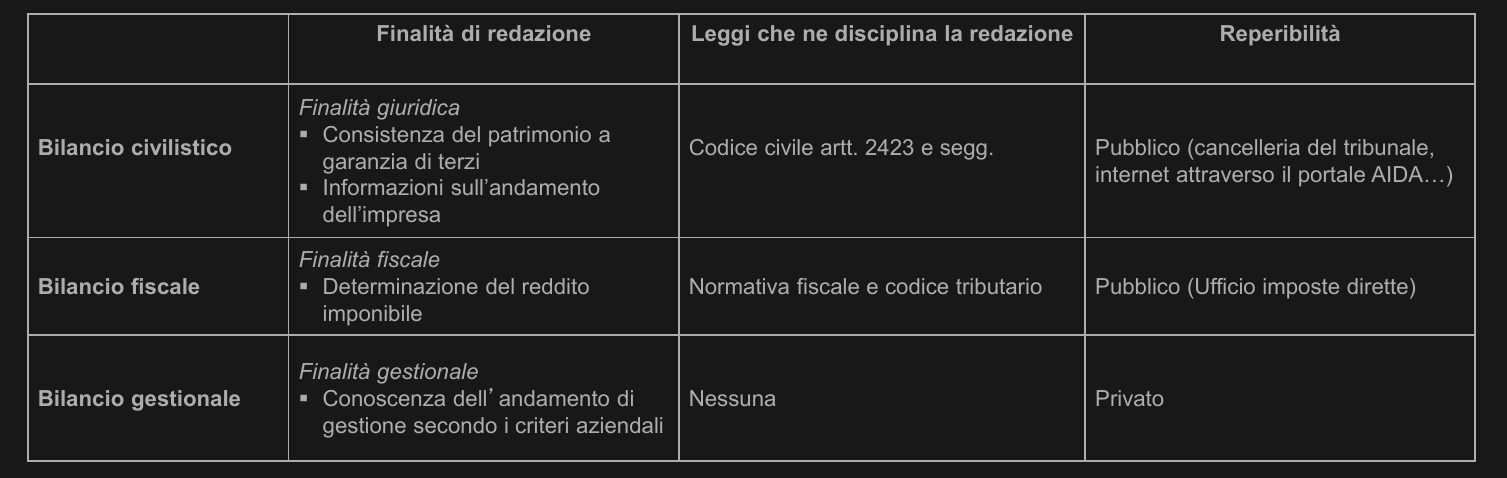
\includegraphics[scale=0.4]{Image/Tabella bilancio.png}
\end{center}
\textbf{N.B.} Il bilancio fiscale si chiude sempre a dicembre, ma un'azienda può compilare un bilancio gestionale (con cadenza arbitraria, as es. mensile o bimestrale) per avere un'idea sui futuri investimenti.


\subsubsection*{I soggetti economici interessati al bilancio}
\begin{itemize}
    \item Portatori interessi
    della comunità locale e
    nazionale
    \item Management e organi di governo
    \item Lavoratori dipendenti
    \item Lavoratori in cerca d'impiego
    \item Banche
    \item Fornitori
    \item Erario
    \item CLienti
    \item Concorrenti
    \item Sindacati
\end{itemize}


\section{I rendiconti economico-finanziari}
\subsection{Bilancio}
Il \textbf{bilancio} è  composto di 4 documenti
principali:
\begin{itemize}
    \item Lo \textbf{Stato Patrimoniale}
    \item Il \textbf{Conto Economico}
    \item Il \textbf{Rendiconto dei flussi di cassa}
    \item La \textbf{Nota Integrativa} (che noi non tratteremo)
\end{itemize}

\subsubsection{Lo stato Patrimoniale}
Lo Stato Patrimoniale rappresenta un'\textbf{istantanea}
della posizione patrimoniale e finanziaria di
un'azienda, cioè la sua posizione in un dato
momento. Esso fornisce tre informazioni essenziali:
\begin{itemize}
    \item che il rendiconto è uno stato patrimoniale\
    \item il nome dell'azienda al quale il rendiconto si riferisce
    \item la data alla quale il rendiconto si riferisce
\end{itemize}
\textbf{Esempio di un rendiconto:}
\begin{center}
    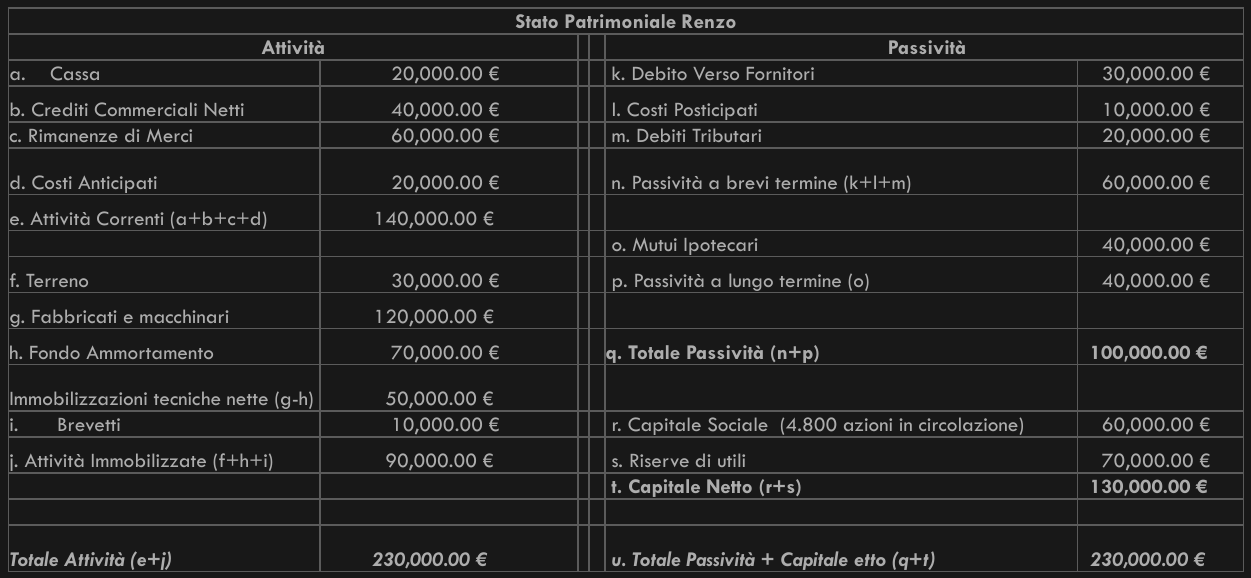
\includegraphics[scale=0.29]{Image/Rendiconto renzo.png
    }
\end{center}
Le \textbf{attività} sono interpretabili come:
\begin{itemize}
    \item Risorse economiche possedute dall'azienda
    \item Impieghi o investimenti aziendali compiuti per perseguire gli obiettivi
aziendali
\end{itemize}
Le \textbf{passività} sono interpretabili come:
\begin{itemize}
    \item Diritti dei creditori nei confronti delle attività aziendali
    \item Obblighi nei confronti dei creditori
    \item Fonti finanziarie messe a disposizione dai creditori
\end{itemize}
Il \textbf{capitale netto} è interpretabile come:
\begin{itemize}
    \item Diritti (residuali) della Proprietà nei confronti delle attività aziendali
    \item Fonti finanziarie messe a disposizione dalla Proprietà
\end{itemize}
L'aumento di capitale netto di un periodo determinato esclusivamente dalle
operazioni di gestione si chiama \textbf{reddito} o \textbf{profitto} o utile (\underline{non} si chiama
guadagno).
\vspace*{0.2cm}\\
Il concetto (formula) da tenere sempre a mente è 
\begin{center}
    ATTIVITÀ = PASSIVITÀ + CAPITALE NETTO
\end{center}



\subsection{Le attività}
\begin{center}
    Le \textbf{attività} sono risorse economiche controllate da un'azienda il cui costo può essere misurato in maniera affidabile al momento dell'acquisizione.
\end{center}
Un'attività deve:
\begin{enumerate}
    \item Essere stata acquisita attraverso una transazione
    \item Essere una risorsa economica
    \item Essere controllata dall'azienda
    \item Il suo costo (o il suo fair value) deve essere misurabile in modo attendibile al momento dell'acquisto
\end{enumerate}
\textbf{N.B.} se un mio pezzo di patrimonio (es. un terreno) subisce una variazione di valore nel tempo questo non viene riportato nello stato patrimoniale.


\subsection{Le attività correnti e le attività
immobilizzate}
\begin{center}
    \renewcommand{\arraystretch}{2}
    \begin{tabular}{|m{5cm}|m{5cm}|}
        \hline 
        \textbf{Attività correnti o attività a breve termine} & \textbf{Attività a lungo termine o immobilizzate}\\
        \hline 
        Attività che si "trasformeranno" in liquidità entro l'esercizio successivo & \multirow{2}{14em}{Immobilizzazioni materiali Immobilizzazioni immateriali  Immobilizzazioni finanziarie}
        \\
        Attività che produrranno la loro utilità entro l'esercizio successivo (di solito l'anno successivo) & \\
        \hline 
    \end{tabular}
\end{center}


\subsubsection{Le attività correnti}
Si definiscono \textbf{correnti} (o a breve termine) le liquidità vere e proprie e,
inoltre, quelle attività che si presume si \textit{trasformeranno} in liquidità entro un anno:
\begin{enumerate}
    \item Liquidità in senso stretto
    \begin{itemize}
        \item Cassa
        \item Conto corrente attivo
    \end{itemize}
    \item Altre attività correnti
    \begin{itemize}
        \item Titoli immediatamente smobilizzabili
        \item Crediti commerciali
        \item Crediti commerciali verso società del gruppo
        \item Crediti finanziari a breve
        \item Rimanenze
    \end{itemize}
\end{enumerate}


\subsubsection{Le attività immobilizzate}
Le attività \textbf{immobilizzate} sono quelle che produrranno la loro utilità su di un arco temporale \underline{pluriennale} o che si
trasformeranno in liquidità in momenti situati \underline{oltre l'esercizio successivo} a quello della data del bilancio.
\begin{enumerate}
    \item Immobilizzazioni \textbf{materiali}
    \begin{itemize}
        \item Terreno
        \item Fabbricati e immobili
        \item Impianti e macchinari
        \item Attrezzature e stampi
        \item Mobili e macchine da ufficio 
    \end{itemize}
    \item Immobilizzazioni \textbf{immateriali}
    \begin{itemize}
        \item Brevetti
        \item Marchi
    \end{itemize}
    \item Immobilizzazioni \textbf{finanziarie} 
    \begin{itemize}
        \item Partecipazioni (strategiche)
        \item Crediti finanziari a lungo termine
    \end{itemize}
\end{enumerate}


\subsubsection{Le immobilizzazioni tecniche}
Sono le immobilizzazioni materiali strumentali allo svolgimento delle operazioni, a esclusione del terreno. Ne sono esempi i fabbricati, i macchinari, gli impianti e le attrezzature, essendo beni intangibili a utilizzo
pluriennale, cioè risorse che si prevede producano la loro utilità su più periodi
amministrativi.
\vspace*{0.2cm}\\
A differenza dei terreni, le immobilizzazioni tecniche hanno vita economica, alla fine della
quale diventano inutilizzabili, ossia non possono più essere considerate un'attività (anche se si continua a utilizzarli).
\vspace*{0.2cm}\\
Il processo di ripartizione del costo d'acquisto di un bene a utilizzo pluriennale tra gli
anni della sua vita utile è denominato \textbf{\color{violet} ammortamento}; al di là della definizione rigorosa, è la percentuale del valore che ogni anno un immobile perde. La vita utile di un'immobilizzazione tecnica è stimata, in genere, da enti preposti, sulla base della quantità di merce prodotta.\\
Alla fine della vita utile, in alcuni casi, le imprese vendono l'immobilizzazione tecnica, denominata \textbf{valore di recupero}.
\begin{center}
    COSTO DA AMMORTIZZARE = COSTO ACQUISTO - VALORE DI RECUPERO
\end{center}


\subsubsection{Le immobilizzazioni immateriali}
\begin{itemize}
    \item CONCESSIONI: diritti attribuiti dalla Pubblica Amministrazione in virtù dei quali l'azienda può: 1. sfruttare beni pubblici quali miniere, suolo demaniale e altro ancora; 2. gestire servizi pubblici in condizioni regolamentate
    \item LICENZE: conferiscono il diritto di: 1. utilizzare a seguito di specifici contratti: software sviluppato da altri; sistemi e procedure commerciali; 2. esercitare un diritto, come per esempio una licenza di gestione di un esercizio pubblico
    \item MARCHI: sono emblemi, denominazioni o segni che caratterizzano i prodotti valorizzando l'immagine dell'azienda sul mercato
    \item BREVETTI: sono diritti in base ai quali le imprese possono impedire ad altri di beneficiare, per un determinato periodo, di un prodotto o di un processo sviluppati con tecnologia originale
    \item AVVIAMENTO: differenza tra il prezzo pagato per l'acquisto di una azienda e il fair value delle attività nette
\end{itemize}


\subsection{Le passività correnti}
\textbf{Passività correnti finanziarie}
\begin{itemize}
    \item Debiti a breve verso banche
    \item Debiti a breve verso società del gruppo
    \item Quote a breve termine di debiti a lungo termine
\end{itemize}
\textbf{Passività correnti operative (di funzionamento)}
\begin{itemize}
    \item Debiti verso fornitori
    \item Cambiali passive commerciali
    \item Debiti tributari
    \item Debiti verso il personale
    \item Costi sospesi
\end{itemize}





\subsection{Le passività a lungo termine}
\begin{itemize}
    \item Prestiti obbligazionari
    \item Mutui (esclusa la quota in scadenza)
    \item Debiti a lungo termine verso società del gruppo
    \item Debiti verso erario a lungo termine
    \item Trattamento di fine rapporto (T.F.R.)
    \item Fondo imposte a lungo termine
\end{itemize}



\subsection{Il capitale netto}
Gli elementi principali costituenti il capitale netto:
\begin{enumerate}
    \item Capitale versato: ammontare di denaro (o beni) apportato direttamente dalla proprietà (azionisti qualora si tratti di una s.p.a.)
    \item Riserve di utili: "ricchezza" generata attraverso la gestione e non distribuita sotto forma di dividendi
\end{enumerate}

\subsection{Esercizio stato patrimoniale}
\begin{center}
    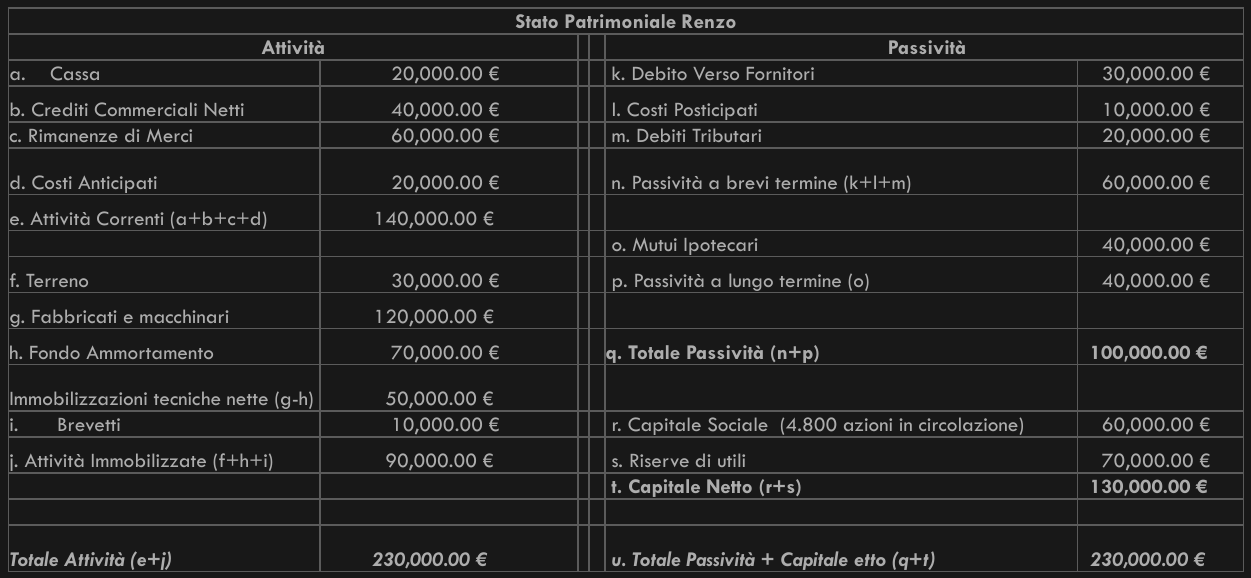
\includegraphics[scale=0.3]{Image/Rendiconto renzo.png}
    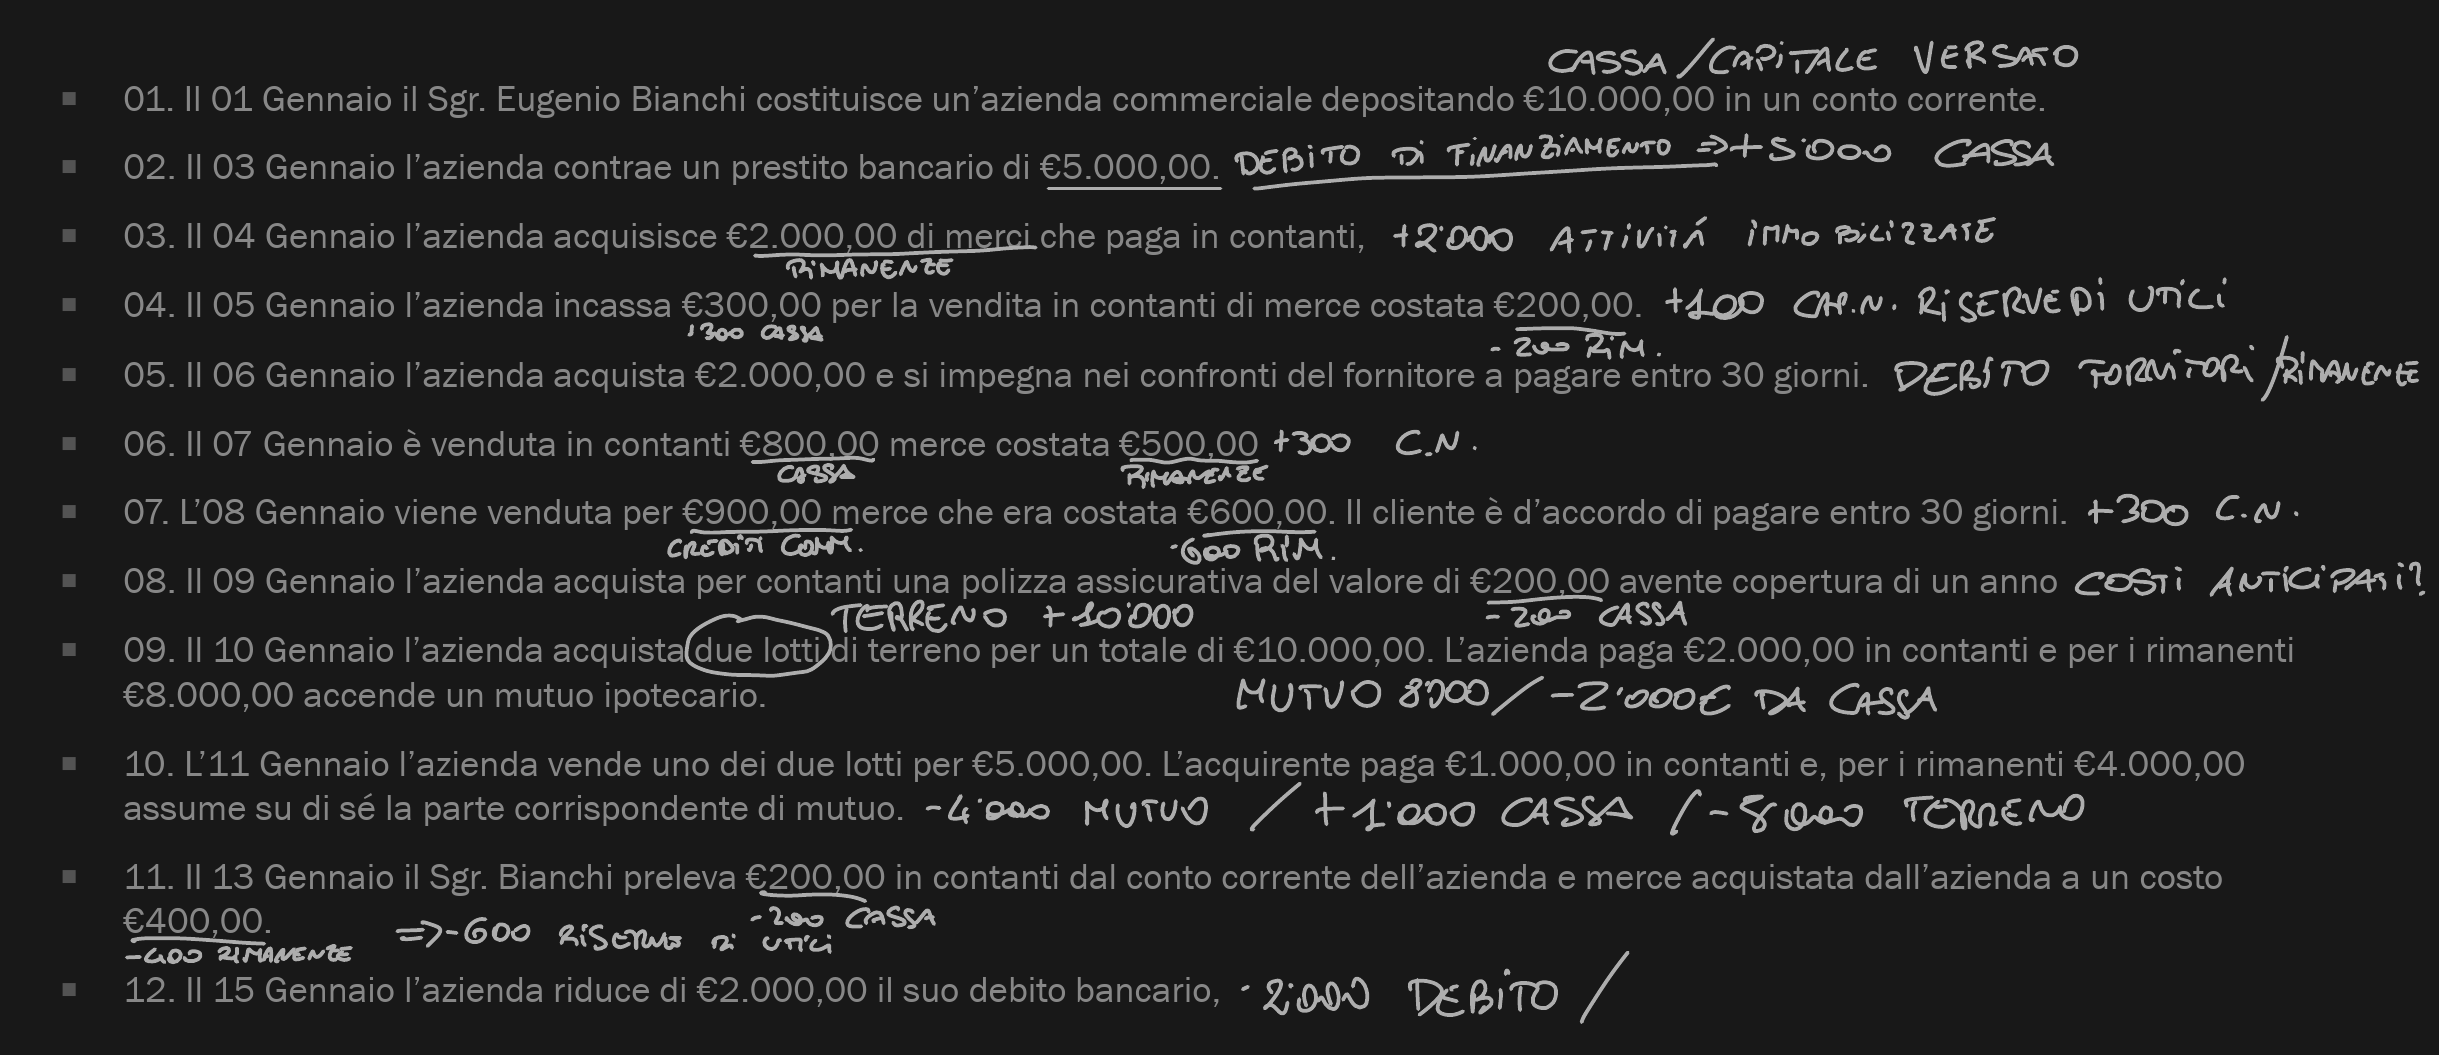
\includegraphics[scale=0.2925]{Image/Esercizio stato patrimoniale_1.png}
\end{center}




\section{Il conto economico e la misurazione dei costi}
\subsection{Il concetto di costo}
Le risorse economiche di un'azienda sono definite \textbf{attività} o \textbf{asset} o elementi patrimoniali.
\vspace*{0.2cm}\\
Le attività possono essere:
\begin{itemize}
    \item \textbf{monetarie}: esiste un'informazione oggettiva e affidabile del loro valore (denaro contante e C/C, titoli, diritti a incassare denaro)
    \item \textbf{non monetarie}: non esiste un'informazione “oggettiva” e affidabile di quale sia il loro valore di mercato (terreni, fabbricati, macchinari)
\end{itemize}
Un'attività, qualunque sia, è normalmente rilevata in contabilità al suo prezzo d'acquisto cioè al suo
costo storico.


\subsubsection*{Attività monetarie}
La maggior parte delle attività monetarie sono registrate in periodi successivi a quello
d'acquisto, tipicamente al loro valore di presunto realizzo o \textit{fair value}.

\subsubsection*{Attività non monetarie}
Il costo d'acquisto continua a essere il riferimento per la contabilizzazione anche nei periodo
successivi.\\
l valore di attività non monetarie, come terreni, fabbricati, non sono correlati con i prezzi ai
quali potrebbero essere venduti, ma \textbf{sono presentati al loro costo storico}.


\subsubsection{Le ragioni del concetto di costo}
Il concetto di costo risulta importante per le attività di un'azienda perché fornisce un'informazione \textbf{relativamente oggettiva} del costo di tale attività.\\
Il concetto consente una \underline{maggiore flessibilità} di valutazione a chi legge un rendiconto.\\
Ciò non significa che il valore di un'attività non monetaria rimanga in
bilancio quello iniziale: il costo storico di un'attività pluriennale è infatti
sistematicamente ridotto nel corso del tempo attraverso l'\underline{ammortamento}.
\begin{center}
    \underline{\textbf{Il principio del costo sacrifica la rilevanza in cambio di una maggiore oggettività e fattibilità}}
\end{center}




\subsection{Il concetto di costo per le attività monetarie}
Le attività monetarie (al pari di quelle non monetarie) sono registrate al costo storico al momento
dell'acquisto o al costo di produzione al momento della loro formazione.\\
Sono poi, nel caso più comune, adeguate nel tempo al loro \textit{fair value}, detto anche \underline{valore di
presunto realizzo}.\\
L'utilizzo del fair value di un'attività monetaria è:
\begin{enumerate}
    \item rilevante
    \item oggettivo
    \item fattibile, cioè a basso costo (ne sono un esempio le azioni quotate)
\end{enumerate}


\subsubsection*{Esempio}
Un'impresa ha investito un surplus di cassa acquistando 100.000 azioni
Unicredit il 30 settembre 2010 al prezzo di €2 e intende determinare il
valore di presunto realizzo dell'investimento al 30 settembre 2012 per
potere redigere il bilancio mensile a quella data. Per far questo è necessario semplicemente attendere la chiusura della
borsa di Milano e leggere sul WEB il valore del titolo. Se, per esempio,
fosse di €3,47, allora il fair value dell'investimento sarebbe di € 347.000 e
non € 200.000.



\subsection{Il concetto di costo per le attività non monetarie}
Il valore di mercato delle attività non monetarie, come terreni, edifici o attrezzature, si modifica nel tempo
per diversi motivi. Il costo d'acquisto (costo storico) non rappresenta dunque, se non al momento dell'acquisto, il valore di
presunto realizzo delle attività non monetarie, non ha cioè un legame con i prezzi ai quali queste
potrebbero essere vendute (fair value); in generale questa differenza cresce col tempo.



\subsection{Spesa, Costo di competenza ed esborso}
\subsubsection{Spesa}
Quando un'azienda acquista beni o servizi sostiene un costo d'acquisto denominato \textit{spesa}; n\underline{non genera una riduzione delle} \underline{riserve di utili}.


\subsubsection{Costo di competenza}
Un'azienda sostiene un costo di competenza quando il
suo capitale netto si riduce a seguito della gestione.
\vspace*{0.1cm}\\
I tipi di costi di competenza sono:
\begin{itemize}
    \item Costi direttamente e analiticamente riconducibili ai ricavi (costo del venduto)
    \item Costi di periodo
    \item Perdite
\end{itemize}


\subsubsection{Esborso}
Esborso è un'uscita di cassa che non necessariamente si
riferisce all'acquisto di un'attività; as esempio il pagamento di un debito con i fornitori.



\subsection{Il Conto economico}
\subsubsection{Ricavi}
Sono flussi in ingresso che risultano dalla vendita di beni o servizi e che si concretizzano in
aumenti di valore di attività (cassa, crediti commerciali ...) e delle riserve di utili.


\subsubsection{Costi di competenza}
Sono flussi in uscita che si concretizzano in riduzioni della cassa (o aumento delle passività) e
di una riduzione delle riserve di utili.
\begin{center}
    Ricavi - Costi di competenza = Reddito
\end{center}
Il reddito può essere indicato come profitto, risultato netto, utile netto.



\subsection{T account}
Le transazioni che durante il periodo amministrativo hanno ripercussioni sul valore della cassa, cioè possono determinare incrementi o decrementi della stessa.\\
La sezione di sinistra, è riservata agli incrementi, mentre l'altra ai decrementi.
\vspace*{0.2cm}\\
Vediamo un esempio:\\ 
\begin{wrapfigure}{r}{0.3\textwidth}
    \centering
    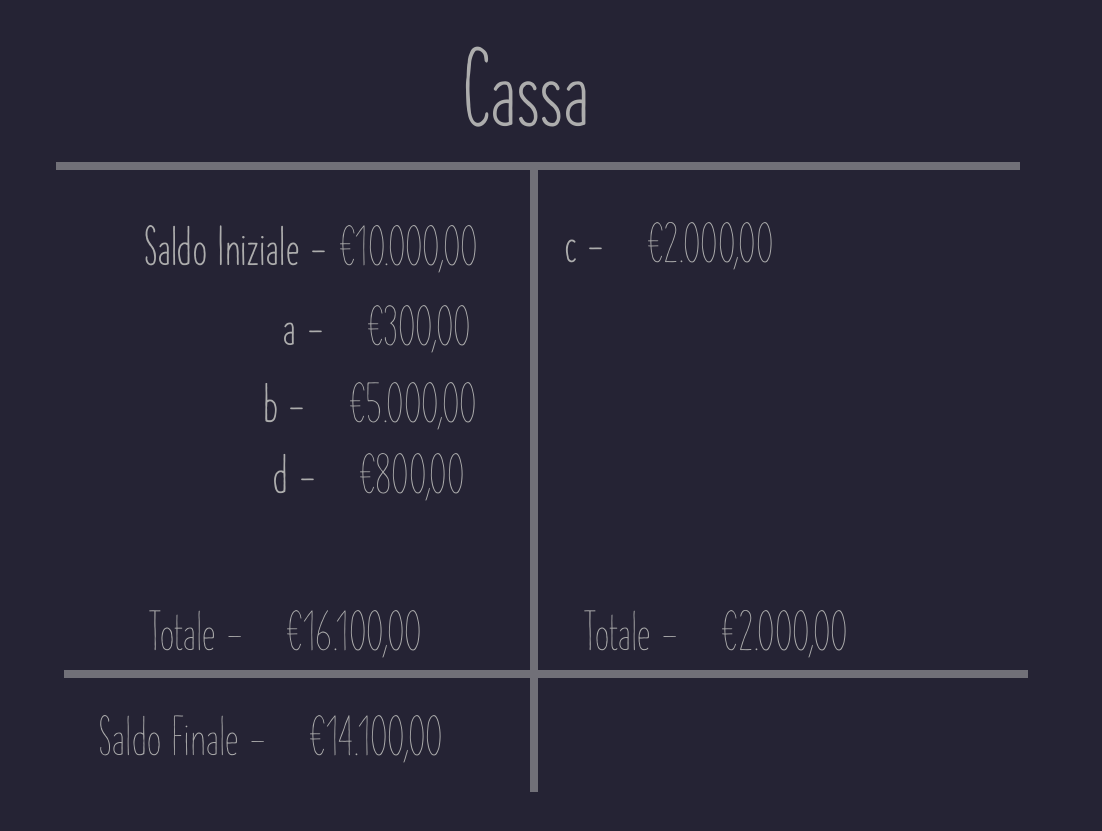
\includegraphics[width=1\linewidth]{Image/Esempio_Taccount_1.png}
\end{wrapfigure}
\begin{itemize}
    \item L'azienda incassa €300,00 per la vendita in contanti di merce costata €200,00
    \item L'azienda contrae un prestito bancario di €5.000,00
    \item L'azienda acquisisce €2.000,00 di merci che paga in contanti
    \item L'azienda vende in contanti €800,00 merce costata €500,00
\end{itemize}
Le regole per gli incrementi e per i decrementi sono:
\begin{itemize}
    \item \textbf{attività:} se "mette" soldi nella cassa va a sinistra; se li "prende" va a destra
    \item \textbf{passività:} si fa il contrario, se "prende" i soldi dalla cassa va a sinistra; se li "mette" va a destra
    \item \textbf{capitale netto:} uguale per le passività
\end{itemize}






\section{Analisi di Bilancio}
L'obiettivo dell'analisi di bilancio:
\begin{itemize}
    \item capire l'andamento economico, patrimoniale e finanziario di un'impresa, nostra o di terzi;
    \item individuare i correttivi da apportare per migliorare l'andamento dell'impresa;
    \item calcolare ed interpretare i rating aziendali;
    \item completare le informazioni di bilancio (Relazione sulla gestione);
    \item controllare le informazioni di bilancio (Relazione del revisore e del Collegio sindacale).
\end{itemize}



\subsection{Indici di Bilancio}
Obiettivo degli Indici di Bilancio:
\begin{itemize}
    \item fornire indicazioni sullo stato di salute dell'azienda;
    \item non rappresentano un punto di arrivo ma un punto di partenza per eventuali correzioni di rotta;
    \item è opportuno poter contare su una pluralità di indicatori;
    \item è indispensabile confrontare nel tempo e nello spazio le informazioni degli indici:
    \begin{itemize}
        \item nel tempo: tra i dati di bilanci di esercizi diversi della stessa azienda;
        \item nello spazio: tra i dati di bilancio dello stesso esercizio di aziende diverse tra loro
        confrontabili (benchmark: medie di settore e best performer).
    \end{itemize}
\end{itemize}


\subsubsection{Classificazione degli Indici di Bilancio}
\begin{center}
    \renewcommand{\arraystretch}{2.5}
    \begin{tabular}{|c|c|}
        \hline
        Redditività & Capacità dell'azienda di creare ricchezza per
        la proprietà\\
        \hline 
        Efficienza & Efficienza nell'utilizzo delle risorse\\
        \hline 
        Liquidità & Capacità dell'azienda di generare (assorbire)
        cassa e di essere solvibile\\
        \hline 
        Struttura finanziaria & Relazione tra i mezzi propri ed i mezzi di terzi \\
        \hline 
        Investment ratio & Performance aziendale nell'ottica dei
        soci/azionisti non operativi\\    
        \hline 
    \end{tabular}
\end{center}


\subsection{Indicatori di Performance}
\begin{center}
    \renewcommand{\arraystretch}{2}
    \begin{tabular}{|p{5cm}|p{5cm}|p{5cm}|}
        \hline 
        \textbf{Indicatori di Performance} & \textbf{Numeratore} & \textbf{Denominatore}\\
        \hline 
        1. Redditività del capitale Netto (ROE) & Reddito Netto & Capitale Netto\\
        \hline 
        2. Utile per Azione & Reddito Netto & Numero di azioni ordinarie in
        circolazione\\
        \hline 
        3. Rapporto prezzo-utili & Valore medio di mercato
        dell'azione & Utile per Azione\\
        \hline
        4. Redditività del capitale investito (ROI) & Risultato Operativo & Fonti di Finanziamento Onerose
        (debiti di finanziamenti + capitale
        netto = capitale investito)\\
        \hline 
    \end{tabular}
\end{center}



\subsubsection{Redditività del Capitale Netto (ROE)}
Il ROE (return of equity) misura il ritorno dell'investimento della proprietà sia direttamente (apporti di capitale) sia indirettamente (riserve utili); fa riferimento al \textbf{reddito netto}. Interessa dunque alla proprietà e potenziali detentori di capitale di rischio, oltre che al management.\\
In altri termini \underline{misura la capacità del patrimonio netto di generare profitti}. 
\[
    \text{ROE} = \frac{\text{Reddito netto}}{\text{Capitale netto}}
\]
Se la società Renzo nel 2021 ha un utile (reddito) netto di
24.000,00 € e un capitale netto di 130.000,00 € il suo ROE sarà del $18\%$ $\left( 24.000,00 \text{€} / 130.000,00 \text{€} \right)$; quindi il capitale  nel 2021 nella Renzo ha avuto un rendimento del $18\%$.
Interpretazione del ROE:
\begin{itemize}
    \item ROE<0: l'azienda sta distruggendo ricchezza
    \item ROE=0: l'azienda non sta creando/distruggendo ricchezza
    \item ROE>0: l'azienda sta creando ricchezza
\end{itemize}



\subsubsection{Redditività del capitale investito (ROI)}
Il ROI (return on investment) ci dice se l'azienda sta impiegando bene il proprio capitale o meno, senza tenere conto di quanto capitale provenga da debiti e quanto da capitale proprio; fa riferimento al reddito \underline{senza imposte}. Interessa dunque alla proprietà e potenziali detentori di capitale di rischio, oltre che al management. Sostanzialmente \textbf{misura la capacità del investimento di generare profitti}.
\[
    \text{ROI} = \frac{\text{Risultato operativo}}{\text{Capitale investito}}
\]
Se la società Renzo nel 2021 ha un risultato operativo di 42.000,00
€ e un capitale investito di 170.000,00 € (40.000,00 € di debiti +
130.000,00 € di capitale netto), il ROI sarà del $25\%$ $\left( 42.000,00 \text{€} / 170.000,00 \text{€} \right)$; quindi il totale investito nel 2021 nella Renzo ha avuto un ritorno del $25\%$.




\subsubsection{Utile per Azione}
L' \textit{utile per azione} Misura il rapporto tra gli utili generati in un certo periodo e il numero di azioni in  circolazione alla fine di quel periodo.
\[
    \text{Utili per Azione} = \frac{\text{Reddito netto}}{\text{Numero di azioni ordinarie in circolazione}}
\]
Ad esempio, nell'azienda "Renzo"
\begin{center}
    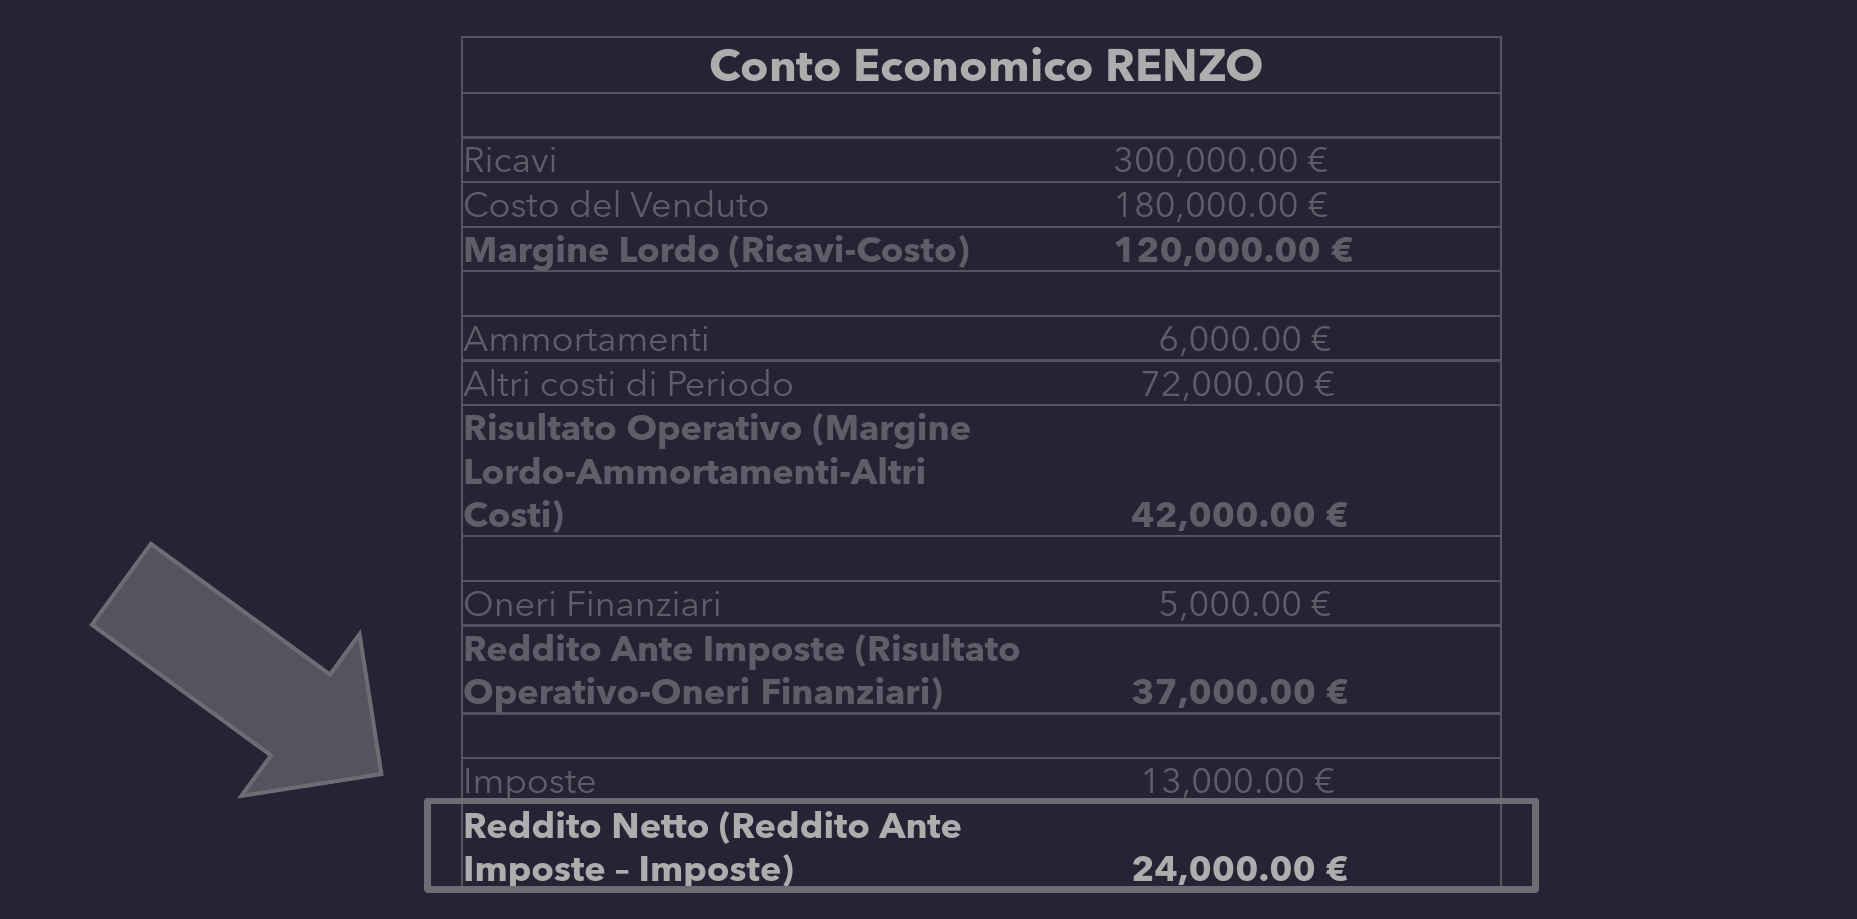
\includegraphics[scale=0.25]{Image/Ce_Renzo.png}
    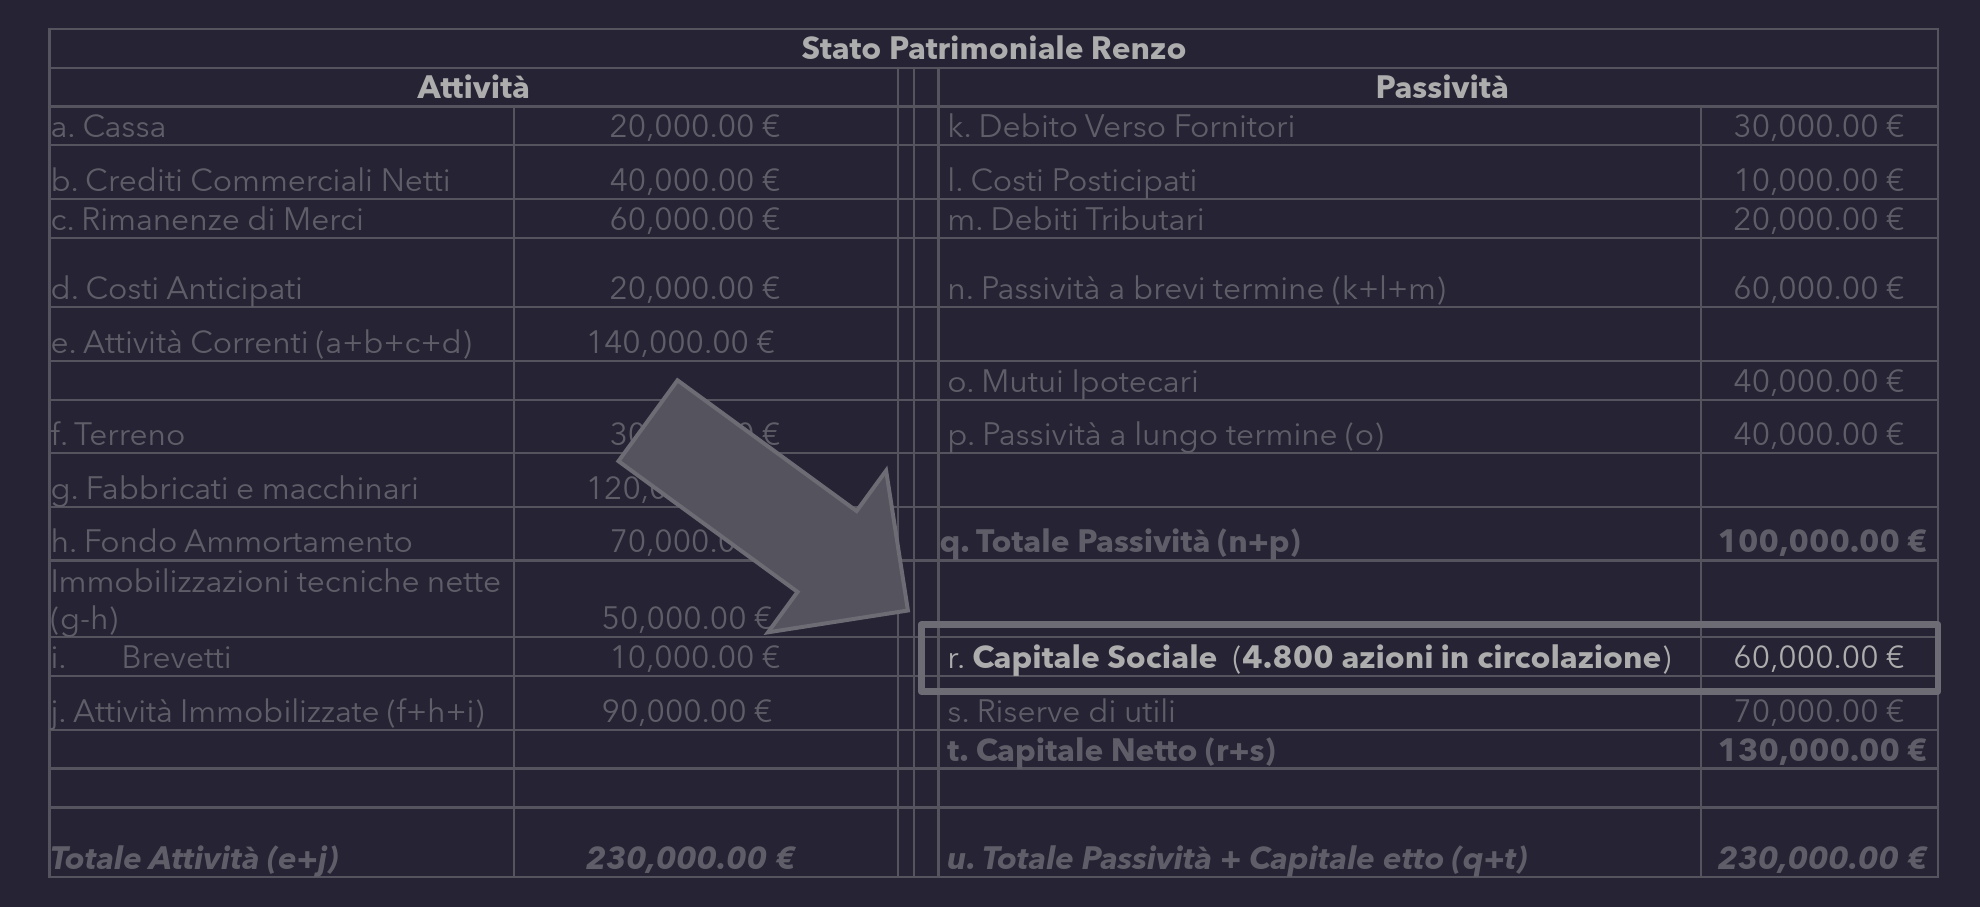
\includegraphics[scale=0.25]{Image/Stato patrimoniale Renzo.png}
\end{center}
\[
    \text{Utili per Azione} = \frac{24.000 \text{\euro}}{4.800 \text{\euro}} = 5 \text{\euro}/\text{azione}
\]

 


\subsubsection{Rapporto prezzo-utili}
Il \textit{rapporto prezzo-utili} (price earnings ratio) misure il rapporto tra il prezzo medio di mercato delle azioni e gli utili per azione come indicativo del valore di una società.
\[
    \text{Rapporto prezzo-utili} = \frac{\text{Valore medio di mercato dell'azione}}{\text{Utile per azione}}
\]
Nel corso di 2020 il prezzo medio di mercato delle azioni di Renzo è stato 35€, abbiamo visto che l'Utile per azione è stato 5€, quindi
\[
    \text{Rapporto prezzo-utili} = \frac{35 \text{\euro}}{5 \text{\euro}} = 7 \text{\euro}
\]
significa che gli investitori pagano 7 \euro per ogni euro di utili correnti.




\subsection{Indicatori di redditività}
\begin{center}
    \renewcommand{\arraystretch}{2}
    \begin{tabular}{|p{5cm}|p{5cm}|p{5cm}|}
        \hline 
        \textbf{Indicatori di Performance} & \textbf{Numeratore} & \textbf{Denominatore}\\
        \hline 
        1. Margine Lordo (\%) & Margine Lordo & Ricavi\\
        \hline 
        2. Risultato Operativo (\%) & Risultato Operativo & Ricavi\\
        \hline 
        3. Reddito Netto (\%) & Reddito Netto & Ricavi\\
        \hline 
    \end{tabular}
\end{center}


\subsubsection{Margine Lordo (percentuale)}
Il \textit{margine lordo (\%)} è il rapporto tra il Margine Lordo e i Ricavi. È una misura del flusso di cassa aziendale, cioè della potenziale capacità dell'azienda di generare cassa con i ricorrenti cicli della gestione operativa (produzione e vendita). Non è quindi una misura di effettiva cassa prodotta ma di potenziale generazione di cassa dell'esercizio.\\
\textbf{N.B.} Un Margine Lordo \% alto non significa un alto valore del reddito netto.
\begin{center}
    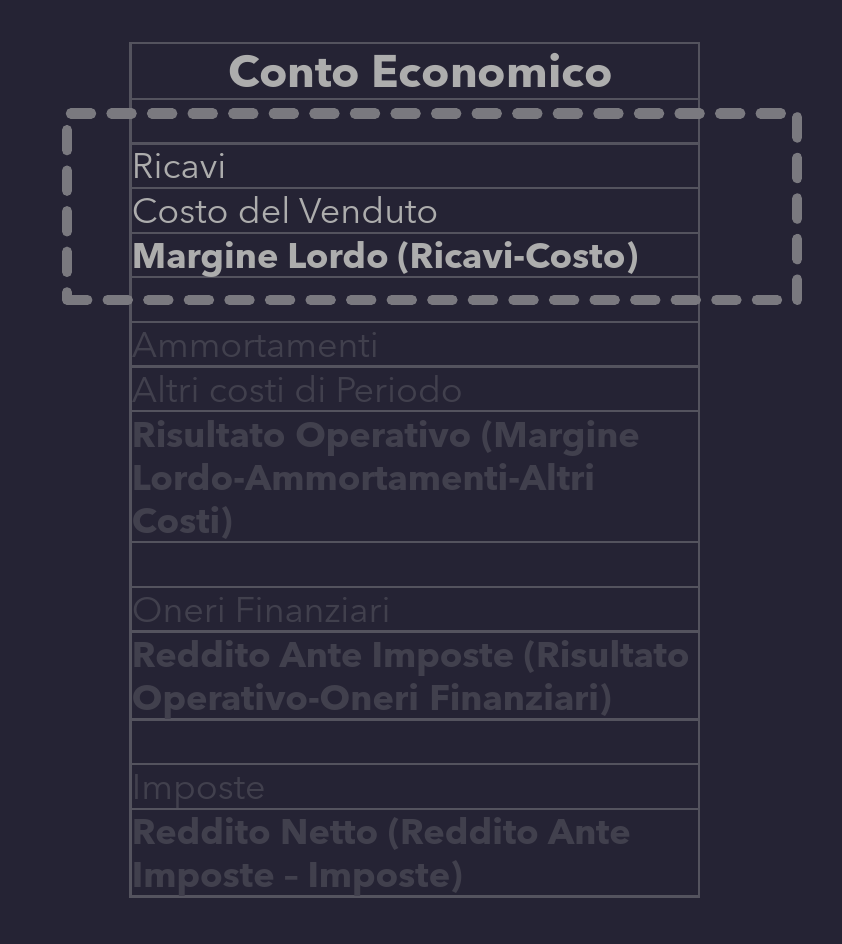
\includegraphics[scale=0.3]{Image/MargineLordo_1.png}
\end{center}
\[
    \text{Margine Lordo \%} = \frac{\text{Margine Lordo}}{\text{Ricavi}}
\]
\begin{center}
    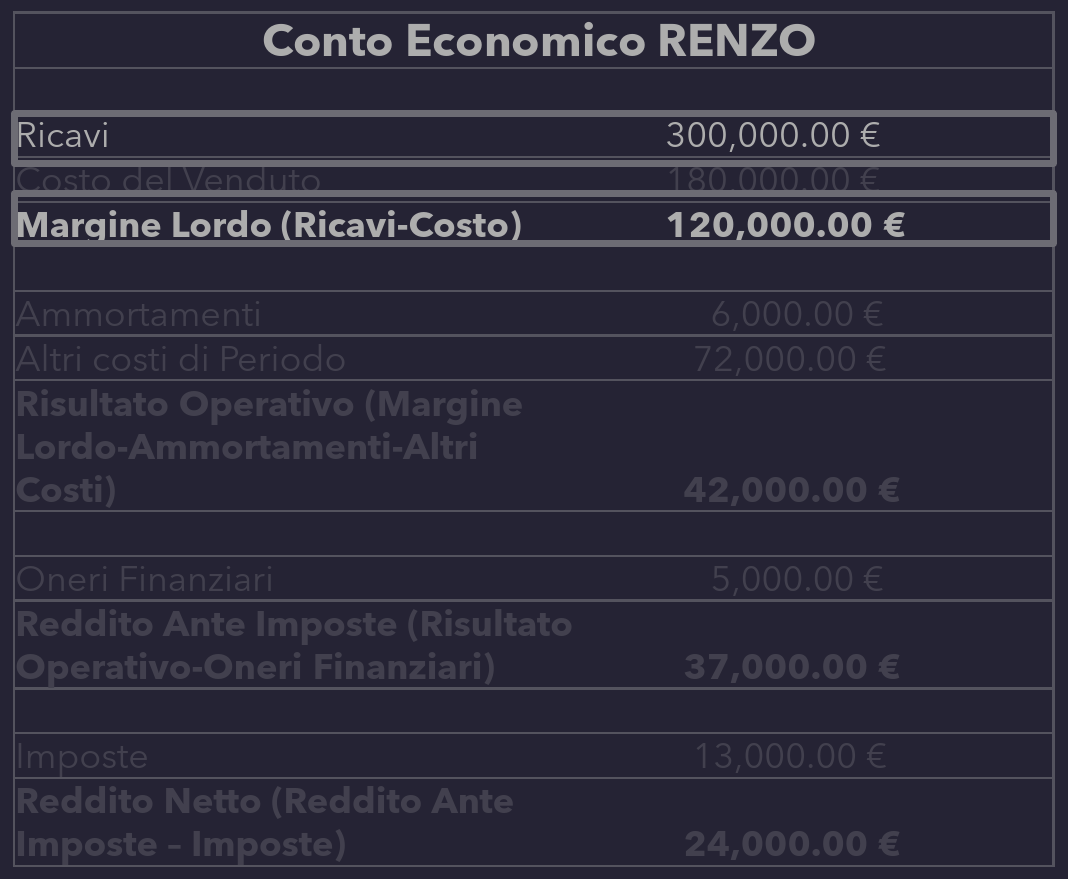
\includegraphics[scale=0.25]{Image/MargineLordo_2.png}
\end{center}
\[
    \text{Margine Lordo \%} = \frac{120.000,00 \text{\euro}}{300.000,00 \text{\euro}} = 40 \%
\]
Il 40 \% del ricavo è il flusso di cassa per coprire altri costi, come debiti, ammortamento e investimento.



\subsubsection{Risultato operativo (percentuale)}
Il risultato operativo misura la capacità di ritorno della produzione dell'impresa. È una misura di adeguatezza della gestione (dato che non considera oneri, debiti e imposte).
\[
    \text{Risultato operativo \%} = \frac{\text{Risultato Operativo}}{\text{Ricavi}}
\]
Ad esempio:
\begin{center}
    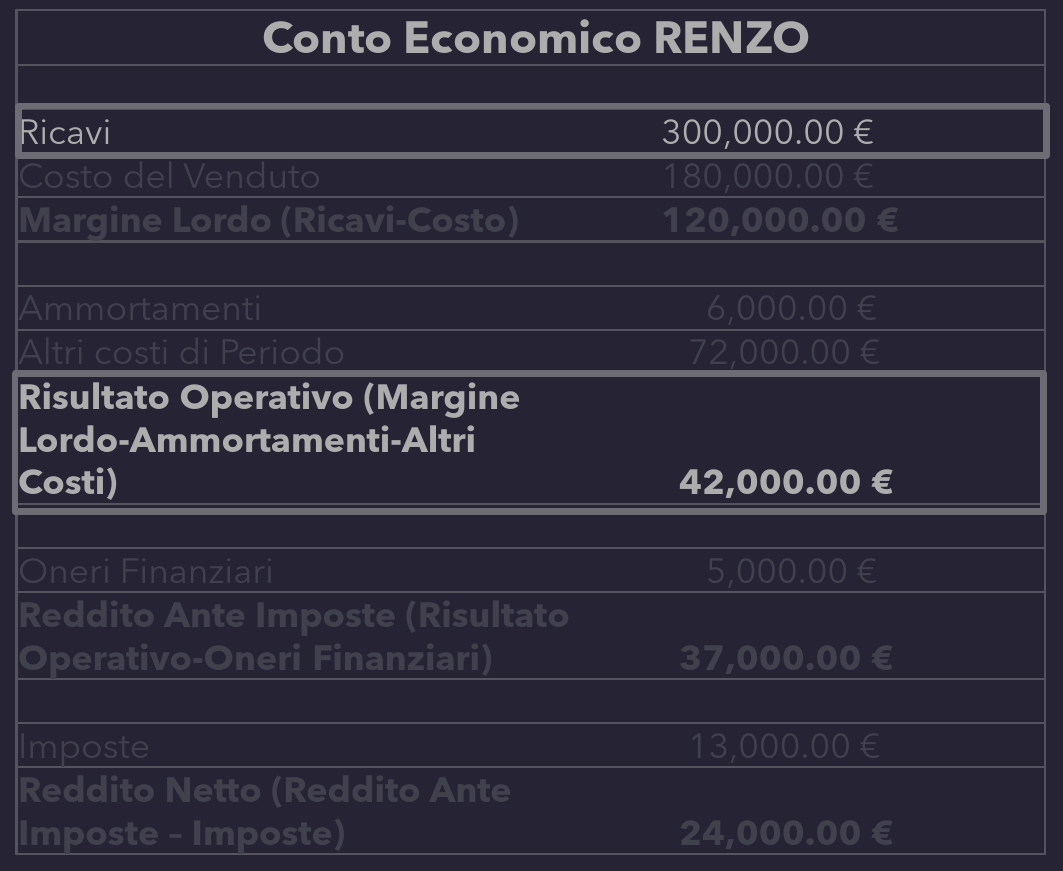
\includegraphics[scale=0.3]{Image/RisultatoOperPer.png}
\end{center}
\[
    \text{Risultato operativo \%} = \frac{42.000,00 \text{\euro}}{300.000,00\text{\euro}} = 14\%
\]


\subsubsection{Reddito netto (percentuale)}
Il reddito netto (percentuale) è una misura di adeguatezza del reddito netto. Misura la capacità di un'azienda di generare utile. È utile conoscerlo dato che ll valore assoluto di reddito netto non permette di analizzare la capacità dell'impresa. I valori medi del reddito netto percentuale dei diversi settori industriali sono disponibili e possono
costituire una base di confronto.
\[
    \T{Reddito Netto \%} = \frac{\T{Reddito Netto}}{\T{Ricavi}}   
\]
Esempio:
\begin{center}
    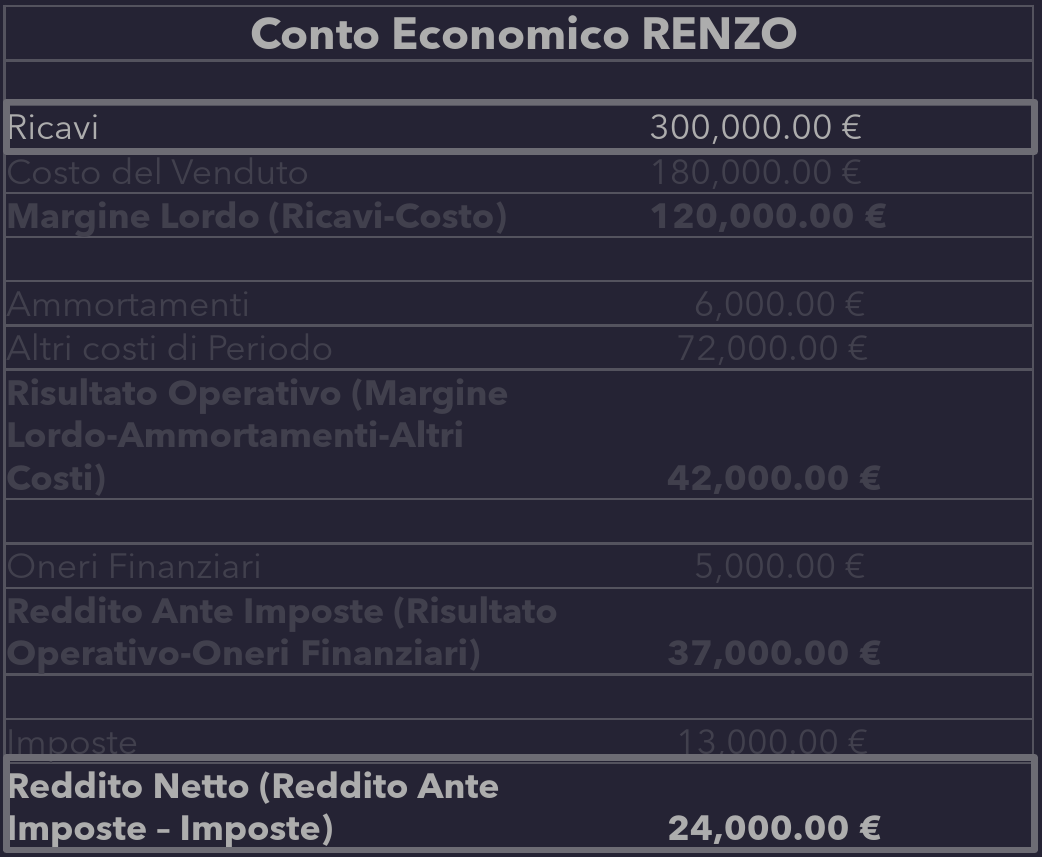
\includegraphics[scale=0.3]{Image/RedditoNettoPerc.png}
\end{center}
\[
    \T{Reddito Netto \%} = \frac{24.000,00\T{\euro}}{300.000,00\T{\euro}} = 8\% 
\]




\subsection{Indicatori di Efficienza di Utilizzo del Capitale}
Gli indicatori di efficienza di utilizzo del capitale misurano la
\textbf{capacità di rendimento e adeguatezza} del capitale investito.\\
Permette di valutare se:
\begin{itemize}
    \item il costo del venduto è adeguato;
    \item come vengono utilizzati i fattori impiegati (input) nel processo di produzione , dato che, se utilizzati
    impropriamente, causano dispersioni di risorse e/o sprechi
\end{itemize}
Sono anche una misura della capacità di rendimento e di rispondenza al
capitale investito.
\vspace*{0.2cm}\\
Vediamo quali sono questi indicatori:
\begin{center}
    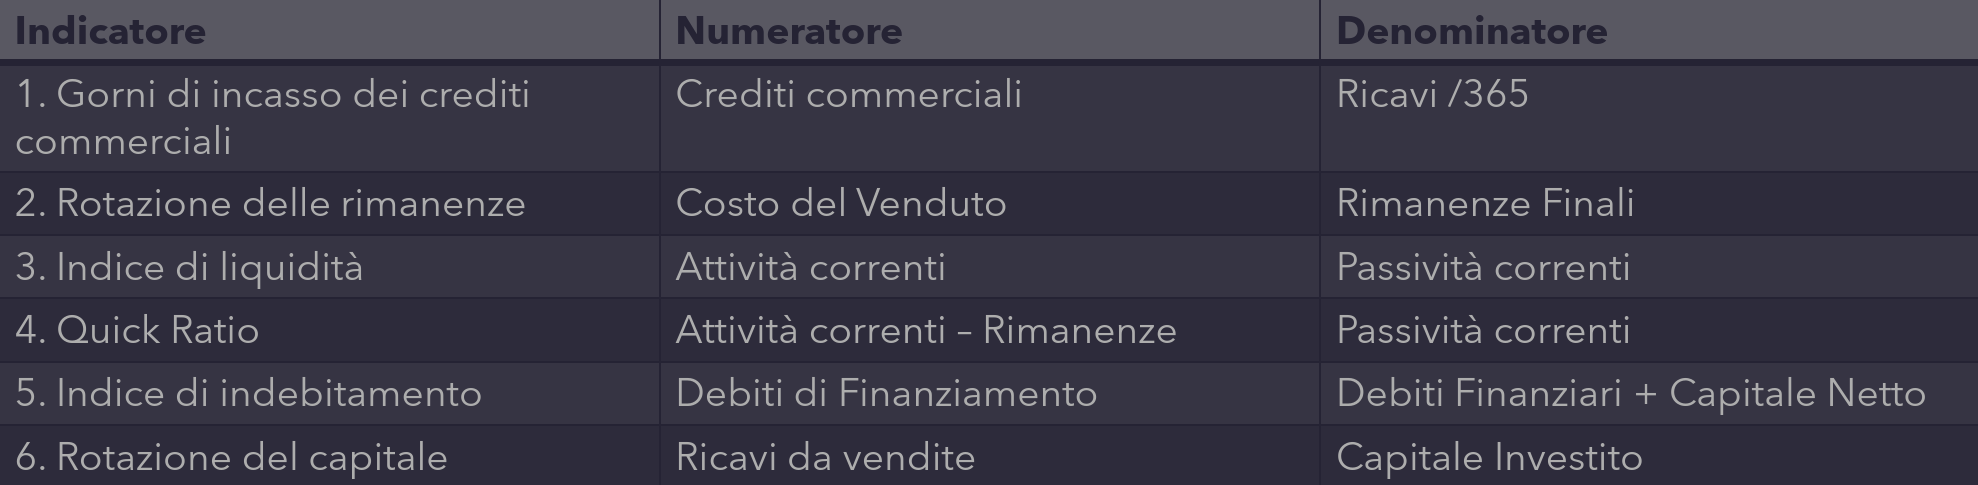
\includegraphics[scale=0.3]{Image/IndicEff.png}
\end{center}



\subsubsection{Giorni di incasso del credito commerciale}
Misura il \textbf{ritardo temporale} tra il momento di realizzazione di ricavi e il momento di incasso del corrispondente credito commerciale.\\
Indica:
\begin{itemize}
    \item se i clienti pagano o meno il loro debito alla scadenza concordata
    \item se le condizioni di incasso peggiorano o
    migliorano nel tempo.
\end{itemize}
\[
    \T{Giorni di incasso del credito commerciale} = \frac{\T{Credito Commerciale}}{\dfrac{\T{Ricavi}}{365}}
\]
Prendiamo in esempio l'azienda Renzo:
\begin{center}
    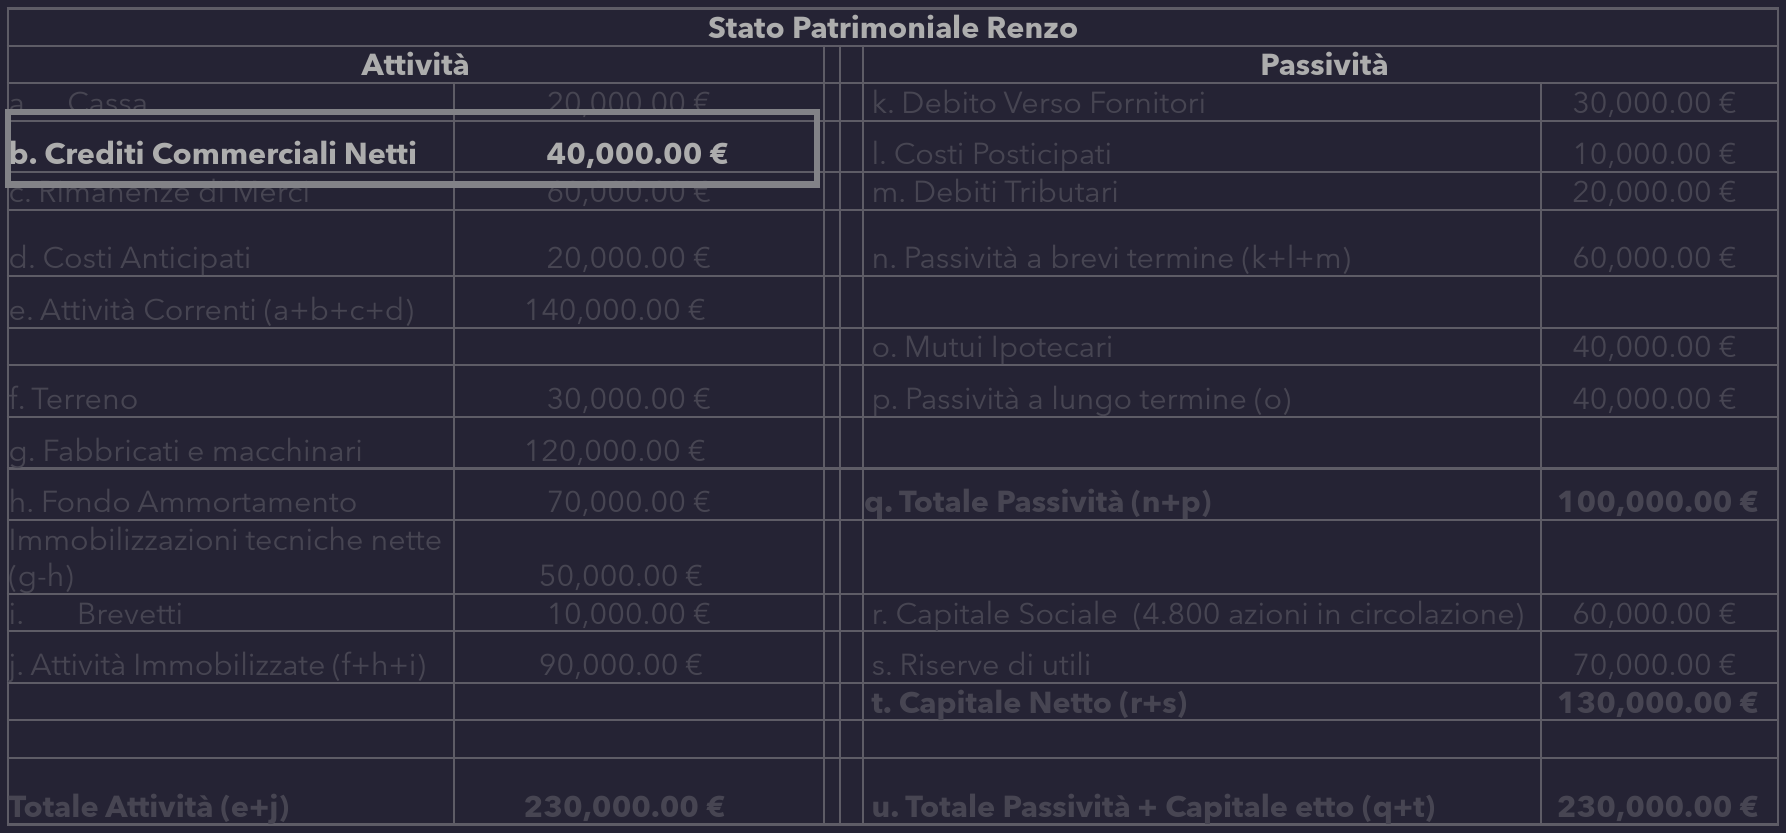
\includegraphics[scale=0.3]{Image/GiorniIncasso_1.png}
    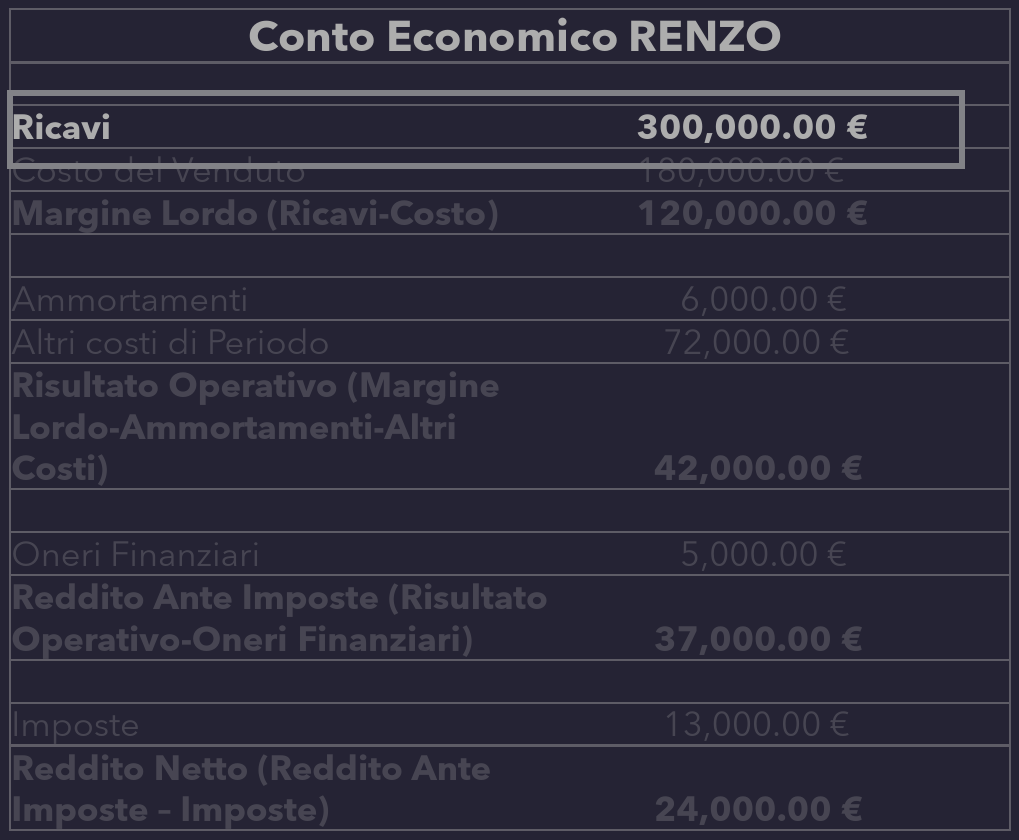
\includegraphics[scale=0.3]{Image/GiorniIncasso_2.png}
\end{center}
\[
    \T{Giorni di incasso del credito commerciale} = \frac{40.000,00 \T{\euro}}{\dfrac{300.000,00\T{\euro}}{365}} = 49 \T{ giorni}
\]



\subsubsection{Rotazione delle rimanenze}
È facilmente intuibile che la \textit{rotazione delle rimanenze} è un indice di \textbf{gestione delle scorte}; esso supporta le decisioni del magazzino, controlli di costo e acquisti. Un \textbf{indice elevato} si ha quando le scorte ruotano molte volte (o velocemente), di conseguenza può causare dei ritardi nei tempi di consegna; mentre, quando l'indice di rotazione è basso le scorte rimangono più "ferme" o ruotano più lentamente, questo vuol dire che le scorte potrebbero divenire obsolete.\\
Sostanzialmente è il \textbf{tempo di giacenza media} di un articolo:
conoscendo l'indice di rotazione si può sapere quanto tempo un articolo rimane in media in magazzino, dal suo ricevimento fino alla vendita.
\[
    \T{Rotazione delle Rimanenze} = \frac{\T{Costo del venduto}}{\T{Rimanenze Finali}}
\]
\begin{center}
    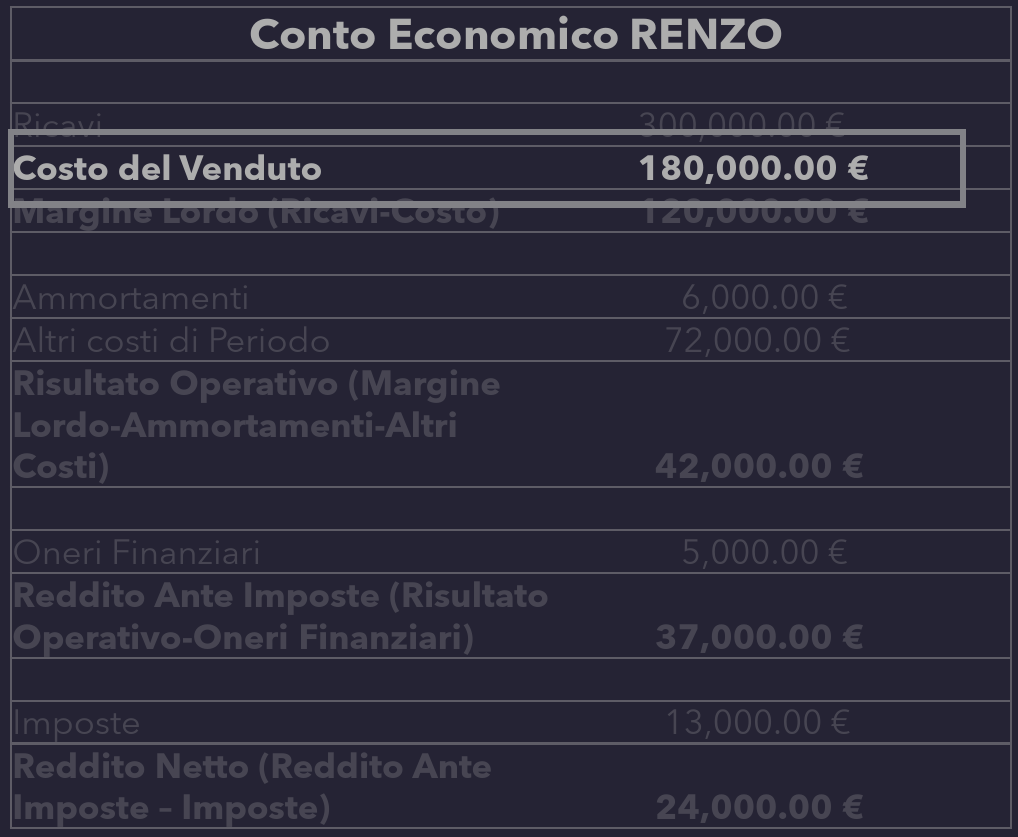
\includegraphics[scale=0.3]{Image/RotazioneRimanenze_1.png}
    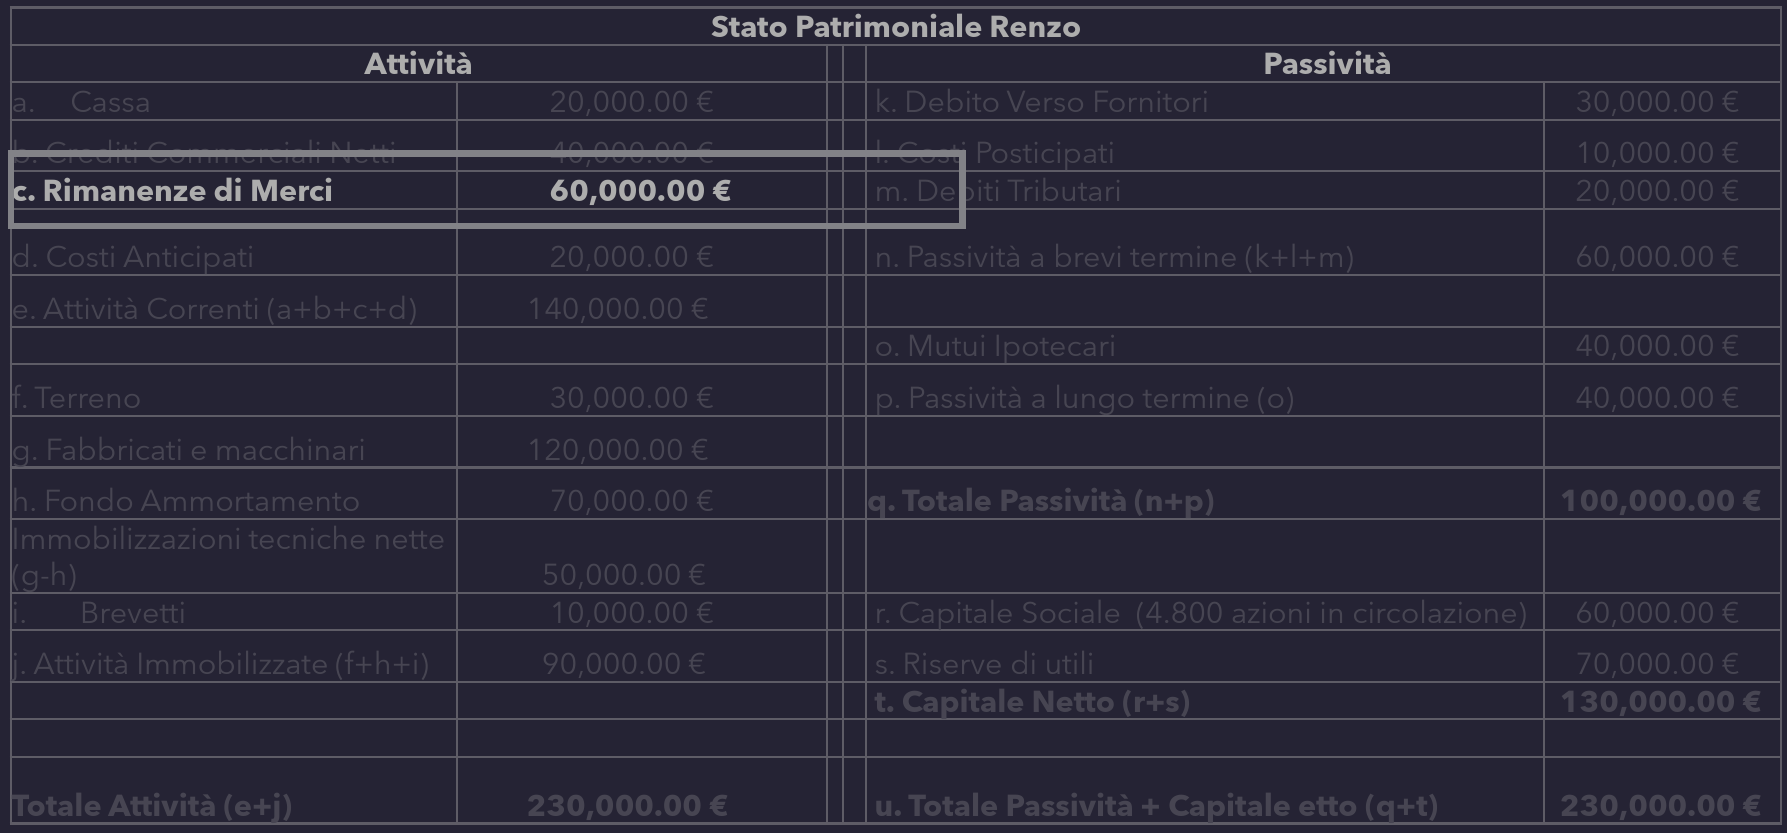
\includegraphics[scale=0.3]{Image/RotazioneRimanenze_2.png}
\end{center}
\[
    \T{Rotazione delle Rimanenze} = \frac{180.000,00\T{\euro}}{60.000,00\T{\euro}} = 3 \T{ (volte)}
\]



\subsubsection{Indice di liquidità}
Permette di valutare l'effettiva capacità dell'impresa nel coprire le uscite a breve termine, queste ultime prodotte dalle passività correnti.
\begin{center}
    \renewcommand{\arraystretch}{2}
    \begin{tabular}{|c|l|}
        \hline
        Indice di liquidità $<1$ & Condizione di insufficienza delle
        disponibilità, rispetto
        all'ammontare dei debiti a breve\\
        \hline
        Indice di liquidità $= 1$ & Disponibilità uguale
        all'ammontare del debito
        aziendale\\
        \hline
        Indice di liquidità $> 1$ & Disponibilità superiore al valore
        dei debiti breve\\
        \hline
    \end{tabular}
\end{center}
\[
    \T{Indice di Liquidità} = \frac{\T{Attività Correnti}}{\T{Passività Correnti}}
\]
Per l'azienda Renzo:
\begin{center}
    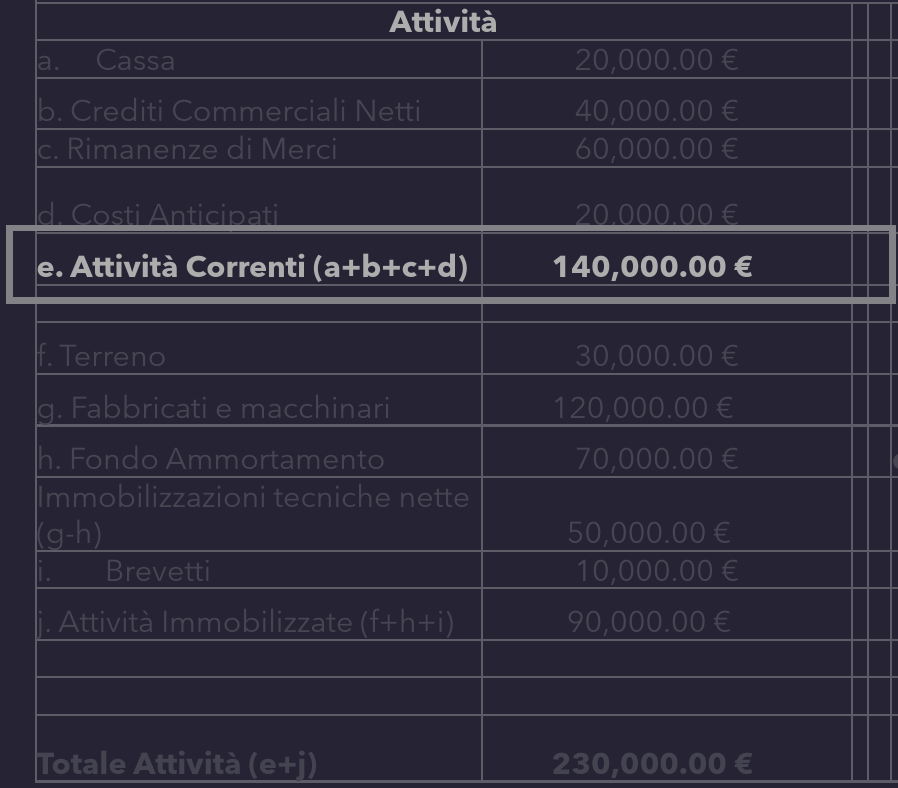
\includegraphics[scale=0.3]{Image/IndiceLiq_1.png}
    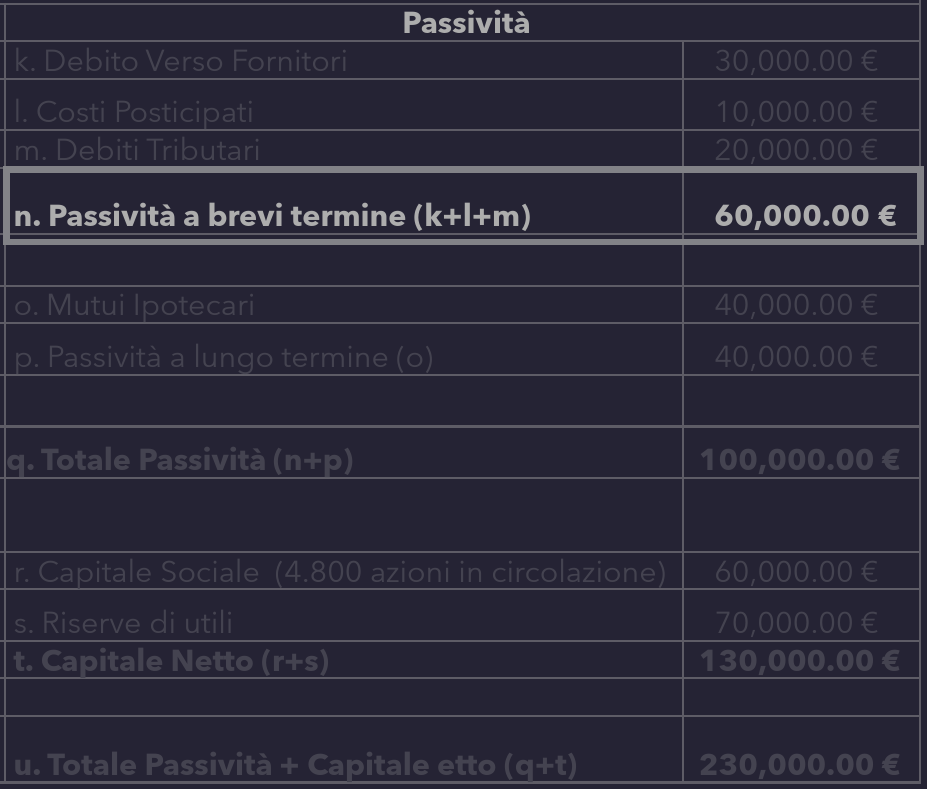
\includegraphics[scale=0.3]{Image/IndiceLiq_2.png}
\end{center}
\[
    \T{Indice di Liquidità} = \frac{140.000,00\T{\euro}}{60.000,00\T{\euro}} = 2,3
\]



\subsubsection{Quick ratio (indice secco di liquidità)}
Misura la capacità immediata di coprire le uscite a breve senza rincorrere alle rimanenze nel magazzino (infatti non vengono considerate nella somma delle attività).
\[
    \T{Quick ratio} = \frac{\T{Attività Correnti - Rimanenze}}{\T{Passività Correnti}}
\]
Esempio per l'azienda Renzo:
\begin{center}
    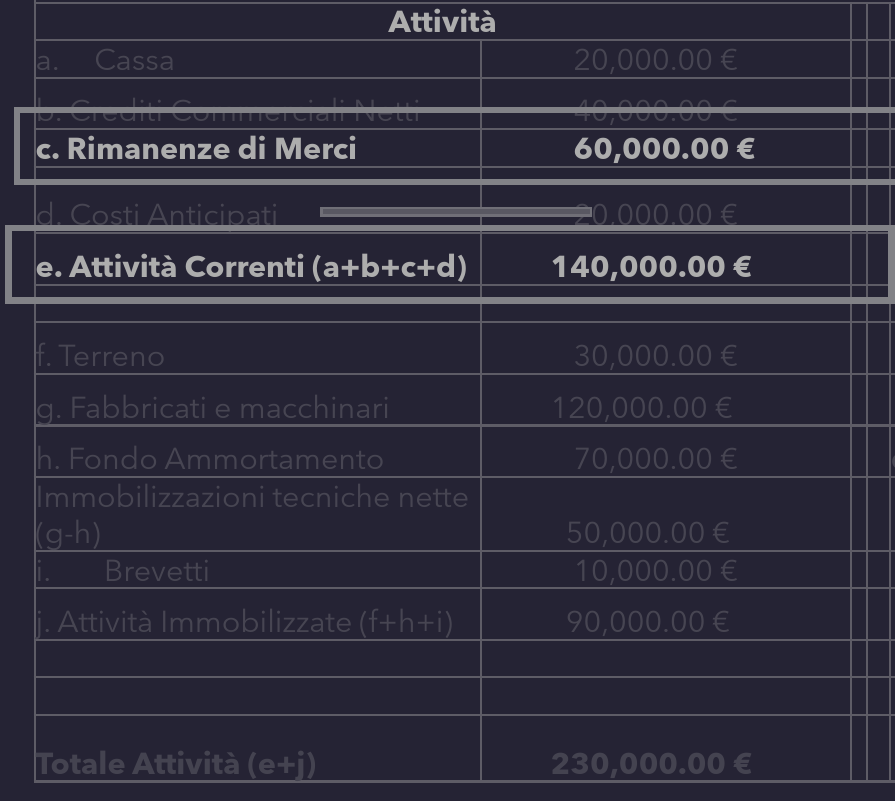
\includegraphics[scale=0.3]{Image/QuickRatio_1.png}
    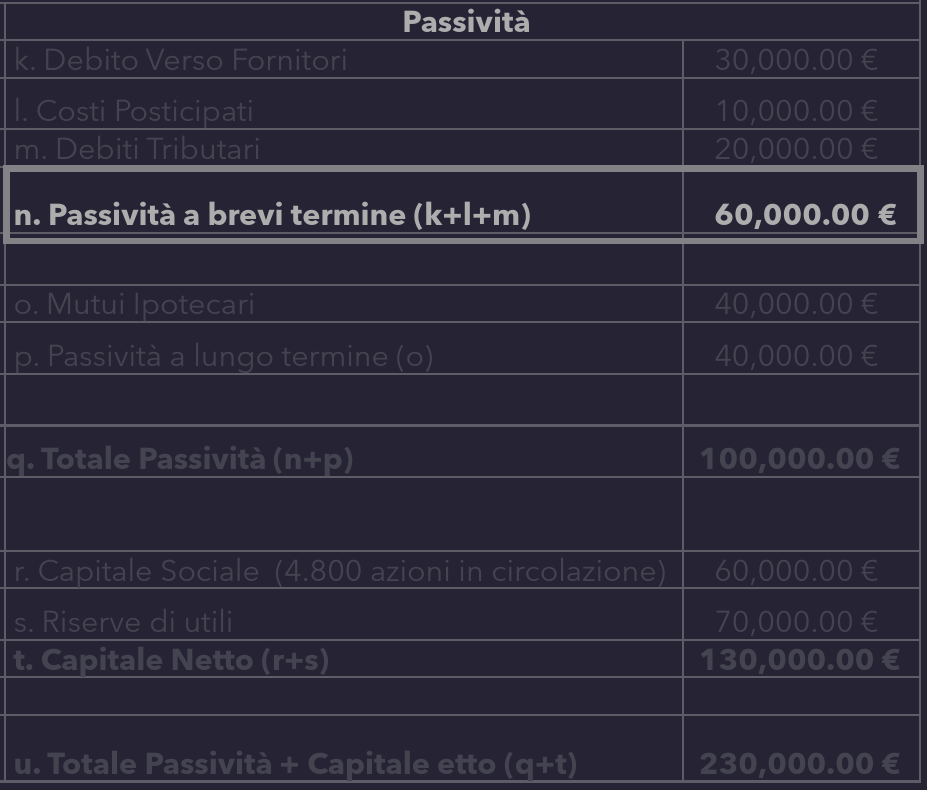
\includegraphics[scale=0.3]{Image/QuickRatio_2.png}
\end{center}
\[
    \T{Quick Ratio} = \frac{140.000,00-60.000,00\T{\euro}}{60.000,00\T{\euro}} = 1,3
\]



\subsubsection{Indice di indebitamento (Debt Ratio)}
Indica la proporzione di fondi presi in prestito che l'azienda ha in
relazione alle fonte di finanziamento (proprio e terzi).\\
L'analisi dipende:
\begin{itemize}
    \item dalla media di comportamento del settore
    \item dal costo e rischio del capitale sociale (costo di opportunità e rischio delle azioni)
    \item dal costo del finanziamento
\end{itemize}
Un indice di Indebitamento molto alto implica una struttura finanziaria più rischiosa.
\vspace*{0.2cm}\\
L'azienda può finanziare le attività attraverso:
\begin{itemize}
    \item le Riserve di Utili, cioè la ricchezza generata attraverso la gestione;
    \item l' apporto di capitale proprio o per le aziende di capitale aperto attraverso le emissioni di nuove azioni;
    \item l' accesso a nuovi debiti di finanziamento.
\end{itemize}
\[
    \T{Debt Ratio} = \frac{\T{Debiti Finanziari}}{\T{Debiti Finanziari + Capitale Netto}}
\]


\subsubsection{Rotazione del Capitale}
Indica quanti euro di ricavo sono stati generati per ciascun euro di capitale investito. Un'azienda che ha un alto investimento in capitale circolante e immobilizzazioni tecniche è denominata impresa \textbf{capital intensive} e si caratterizza per valori bassi di rotazione del capitale investito.\\
\textbf{N.B.} Il Capitale Investito è l'aggregato del capitale netto e dei debiti di finanziamenti.

\[
    \T{Rotazione del Capitale} = \frac{\T{Ricavi}}{\T{Capitale investito}}
\]
Esempio:
\begin{center}
    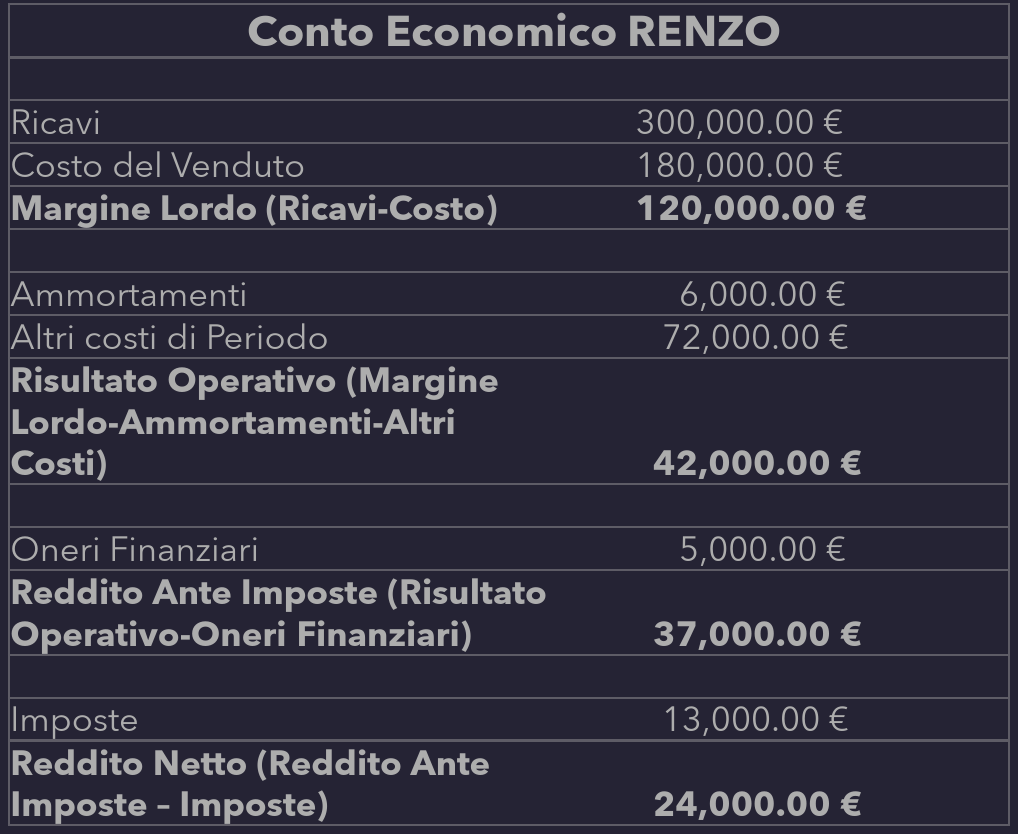
\includegraphics[scale=0.3]{Image/RotCapitale_1.png}
    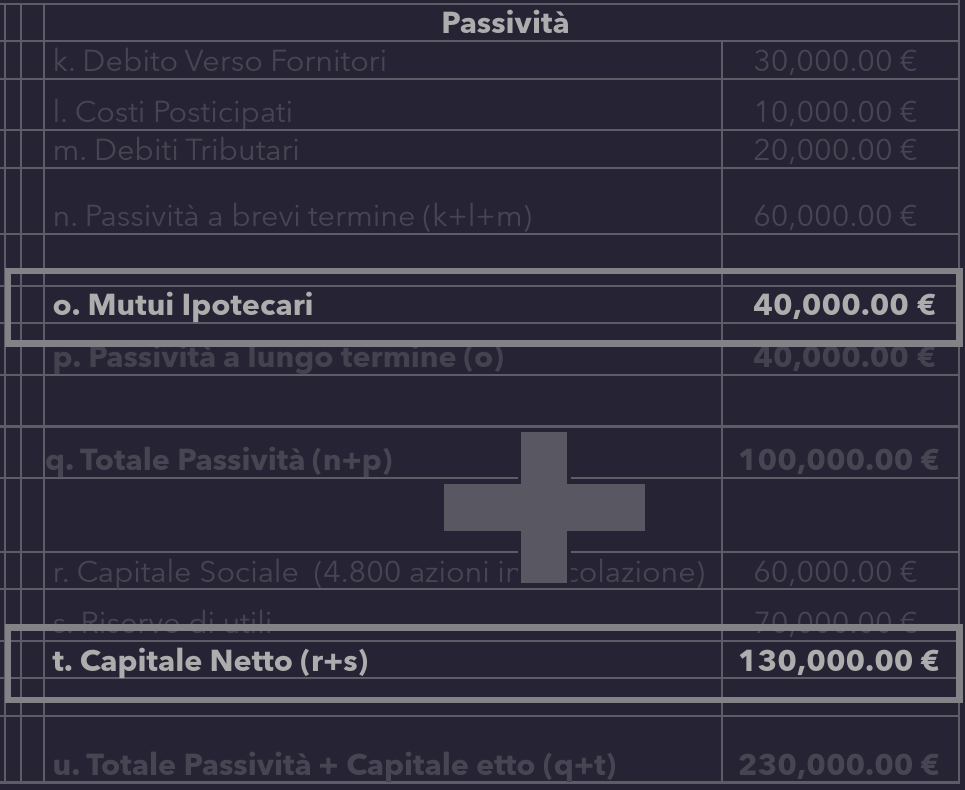
\includegraphics[scale=0.3]{Image/RotCapitale_2.png}
\end{center}
\[
    \T{Rotazione del Capitale} = \frac{300.000,00\T{\euro}}{40.000,00\T{\euro}+ 130.000,00 \T{\euro}} = 1,80 \T{\euro}
\]
L'azienda ha generato $1,80 \T{\euro}$ di ricavo per ciascun euro di capitale investito.
\vspace*{0.2cm}\\
Un'altra alternativa per misurare la \underline{Redditività del Capitale Investito} (ROI) è moltiplicare il risultato percentuale operativo per l'indice di rotazione del capitale.
\[
    \frac{\T{Risultato Operativo}}{\T{Ricavi}} \times \frac{\T{Ricavi}}{\T{Capitale investito}} = \frac{\T{Risultato Operativo}}{\T{Capitale investito}}
\]









\section{Management Accounting}
\subsection{Contabilità generale vs contabilità direzionale}
\begin{itemize}
    \item Contabilità Generali: è preparata soprattutto per attori
    esterni all'impresa. Le informazione assistono i finanziatori
    nella valutazione delle prospettive di redditività dell'impresa;
    \item Contabilità Direzionale: è preparata per supportare le
    decisioni interne. Fornisce le informazioni utilizzate per
    pianificare, porre in atto e controllare le attività di
    un'organizzazione. Le informazione di contabilità direzionale
    sono riepilogative, ottenute assemblando dati elementari
    operativi.
\end{itemize}

\subsubsection{Tre tipiche funzioni del management}
\begin{itemize}
    \item Programmare:
    \begin{itemize}
        \item decidere quali azioni debbano essere avviate (\textbf{decision making});
        \item il budget è il processo di programmazione per un determinato periodo, normalmente un anno;
        \item la pianificazione ha un orizzonte pluriennale.
    \end{itemize}
    \item Implementare:
    \begin{itemize}
        \item porre in atto azioni
        necessarie affinché
        attraverso risorse e
        persone si possano
        conseguire i risultati
        programmati
        \item richiede supervisione
        \item i manager possono
        modificare i programmi
        quando risulti necessario
        od opportuno
    \end{itemize}
    \item Controllare:
    \begin{itemize}
        \item il processo volto a
        ottenere dalle persone le
        azioni e i comportamenti
        desiderati
        \item le informazioni contabili
        sono utilizzate per:
        \begin{itemize}
            \item comunicare
            \item motivare
            \item indirizzare l'attenzione
            \item valutare
        \end{itemize}
    \end{itemize}
\end{itemize}
\begin{center}
    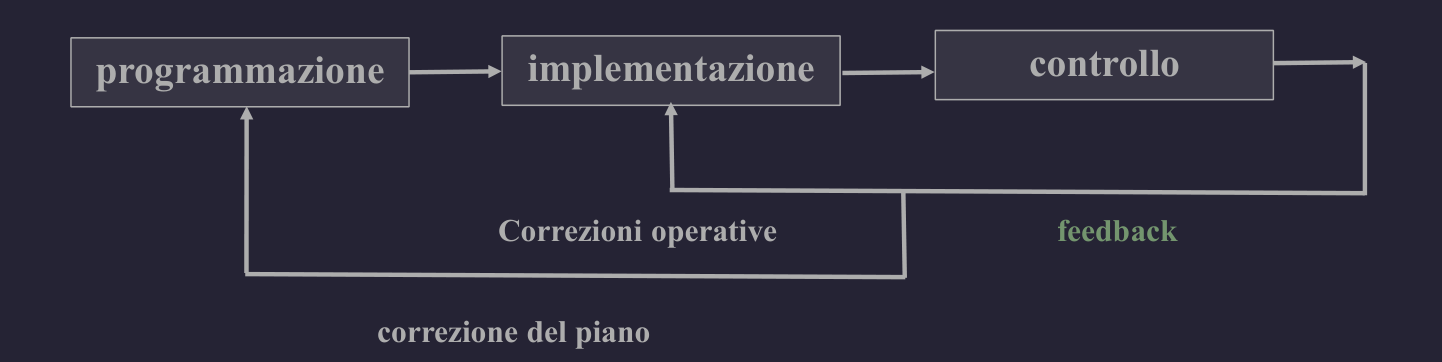
\includegraphics[scale=0.3]{Image/FunzioniManag_1.png}
\end{center} 
\textbf{N.B.} La contabilità direzionale fornisce la gran parte delle informazioni monetarie e quantitative utilizzate dal management per programmare, porre in atto le decisioni e controllare.
\begin{center}
\renewcommand{\arraystretch}{2.5}
\begin{tabular}{|l|m{5cm}|m{5cm}|}
    \hline
    \textbf{\color{synthwave_text}Caratteristiche} & \textbf{\color{synthwave_text}Contabilità Generale} & \textbf{\color{synthwave_text}Contabilità Direzionale}\\
    \hline 
    01. Necessità d'uso &Obbligatoria &Facoltativa\\
    \hline 
    02. Finalità&Produrre Informazioni per l'esterno&Strumento per assistere il management\\
    \hline 
    03. Utilizzatori&Gruppi relativamente ampi dall'identità ignota&Gruppi relativamente ristretti dall'identità nota\\
    \hline 
    04. Struttura Sottostante&Equazione fondamentale del bilancio&Cambia in funzione dell'utilizzo delle informazioni\\
    \hline 
    05. Fonte dei principi&Codice Civili e Principi Contabili&Qualunque essa sia, purché ritenuta utile\\
    \hline 
    06. Prospettiva Temporale&Storica&Storica e Prospettica\\
    \hline 
    07. Tipo delle informazioni&Prevalentemente Monetarie&Monetarie e non Monetarie\\
    \hline 
    08. Precisione delle Informazioni&Livello relativamente alto&Livello relativamente basso\\
    \hline 
    09. Frequenza del reporting&Trimestrale e annuale&Cambia con lo scopo\\
    \hline 
    10. Tempestività del reporting&Ritardi di settimane e anche di mesi rispetto al periodo esaminato&Report prodotti tempestivamente al termine del periodo di misurazione\\
    \hline 
    11. Oggetto del reporting&L'intera impresa&Unità organizzativa\\
    \hline 
    12. Responsabilità&Teoricamente sempre presenti&Virtualmente Nessuna\\
    \hline 
\end{tabular}
\end{center}



\subsection{Similarità tra contabilità generale e contabilità direzionale}
\begin{enumerate}
    \item i criteri generali sono condivisi: molti criteri generali alla base dei principi contabili sono rilevanti anche nella contabilità direzionale (ad esempio il principio del costo storico);
    \item molti dati elementari sono condivisi: gran parte dei dati elementari utilizzati dalla contabilità generale e raccolti in conformità ai principi contabili sono utilizzati anche dal contabilità direzionale;
    \item scopo comune: entrambi i tipi di informazione sono utilizzati per fini decisionali.
\end{enumerate}



\subsection{Scopi e usi delle informazioni della contabilità direzionale}
Gli \underline{scopi} delle informazioni della contabilità direzionale sono:
\begin{itemize}
    \item misurazione dei ricavi, dei costi e delle attività;
    \item controllo;
    \item supporto nelle scelte di alternative
\end{itemize}
Per ognuno dei tre scopi esistono un insieme specifico di principi e di generalizzazioni e tre corrispondenti modalità di costruire i costi:
\begin{itemize}
    \item[$\blacktriangleright$] Le configurazioni di costo pieno (full cost accounting)
    \item[$\blacktriangleright$] Le configurazioni di costo per centro di responsabilità (responsibality accounting)
    \item[$\blacktriangleright$] Le configurazioni di costo differenziale (differential accounting)
\end{itemize}
\begin{center}
    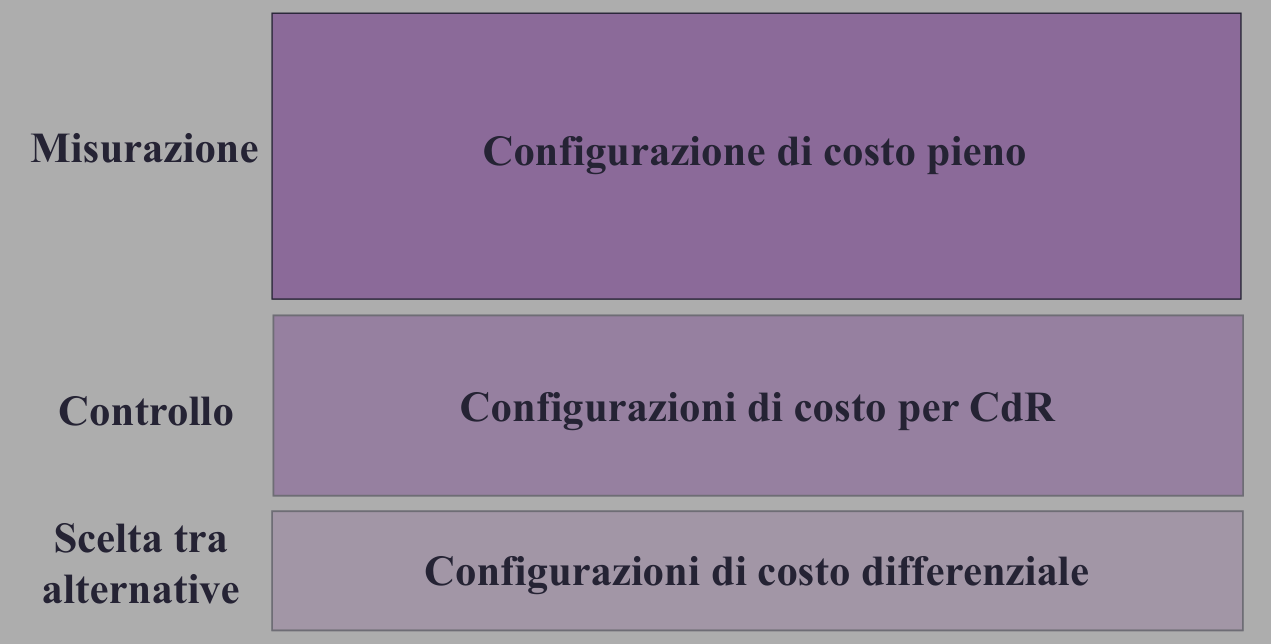
\includegraphics[scale=0.3]{Image/ScopiContDirez_1.png}
\end{center}


\subsubsection{Scopo 1: la misurazione}
Il costo pieno è la somma dei costi diretti e una quota equa dei
costi indiretti (può riferirsi a qualsiasi oggetto).
\vspace*{0.2cm}\\
I costi pieni sono rilevati soprattutto per:
\begin{itemize}
    \item valorizzare le rimanenze
    \item determinare prezzi (anche di servizi pubblici) regolamentati da contratto
    \item essere il riferimento per la determinazione dei prezzi “normali”
    \item misurare la redditività di prodotti/mercati/clienti etc...
    \item misurare la redditività dei centri di profitto (divisioni)
\end{itemize}


\subsubsection{Scopo 2: il controllo}
I costi per Centro di Responsabilità (CdR) sono rilevati soprattutto
per:
\begin{itemize}
    \item valutare la performance dei responsabili dei CdR
    \item valutare la redditività dei CdR
    \item motivare (premi e bonus collegati alla performance)
    \item supportare il processo di budget
\end{itemize}


\subsubsection{Scopo 3: Il supporto alle decisioni}
I costi differenziali o rilevanti:
\begin{itemize}
    \item sono quelli che cambiano da un'alternativa all'altra
    \item dipendono dal tipo di decisione
    \item non sono normalmente presenti all'interno del sistema contabile
\end{itemize}


\begin{center}
    \begin{tabular}{|l|m{5cm}|m{5cm}|}
        \hline
         & \multicolumn{2}{|c|}{\textbf{\color{synthwave_text}Modalità di utilizzo}}\\
        \hline
        \textbf{\color{synthwave_text}Scopo} & (in base a valori consuntivi) & (in base a stima di valori futuri)\\ \hline
        \multirow{4}{*}{\color{synthwave_text}\textbf{Misurazione}} & Valorizzare le rimanenze & \multirow{4}{*}{Definizione dei prezzi "normali"}\\
        & Calcolare prezzi regolamentati & \\
        & Analizzare al redditività dei prodotti & \\
        & Analizzare le prestazioni dei CdR &\\
        \hline
        \multirow{2}{*}{\color{synthwave_text}\textbf{Controllo}} & Analizzare le performance manageriali & Pianificazione strategica\\
        & Motivare e premiare i manager & Budgeting\\
        \hline 
        \multirow{2}{*}{\color{synthwave_text}\textbf{Scelta tra alternative}} & Non utilizzati & Decisioni di breve periodo\\
        & & Decisioni di lungo periodo\\
        \hline 
    \end{tabular}
\end{center}
\textbf{N.B.} Consuntivo: rendiconto, sia delle imprese sia degli enti pubblici, dei risultati di un dato periodo di attività.




\subsection{La classificazione dei costi}
\subsubsection{Differenza dei costi}
I costi \textit{variano} a seguito di cambiamenti dei livelli di output. È importante sapere individuare quali costi saranno modificati dalle decisioni e stimare di quanto si modificheranno.
\vspace*{0.2cm}\\
Esiste un'ovvia relazione tra \textbf{costi} e \textbf{volumi}: se i volumi aumentano aumentano anche i costi. Attenzione però, perché in termini percentuali l'incremento dei costi può essere più basso dell'incremento del volume.\\
Quando parliamo di costi bisogna distinguere tra \textbf{costi fissi}, \textbf{costi variabili} e \textbf{costi semi-variabili}.


\subsubsection{Costi variabili}
I \textit{costi variabili} sono costi il cui valore complessivo varia in misura direttamente proporzionale a un qualche livello di attività o di output. La causa del cambiamento del costo si chiama determinante del costo (\textit{cost driver}). La programmazione e il controllo dei costi variabili richiedono la conoscenza di tutti i cost drivers.
\vspace*{0.2cm}\\
Le determinanti dei costi variabili possono essere molteplici:
\begin{itemize}
    \item il carburante per il numero di km percorsi o le ore di volo;
    \item le materie prime per il numero di prodotti finiti;
    \item per le provvigioni l'ammontare dei ricavi realizzati;
    \item per l'assistenza tecnica il numero di ore di servizio prestate.
\end{itemize}

\begin{center}
    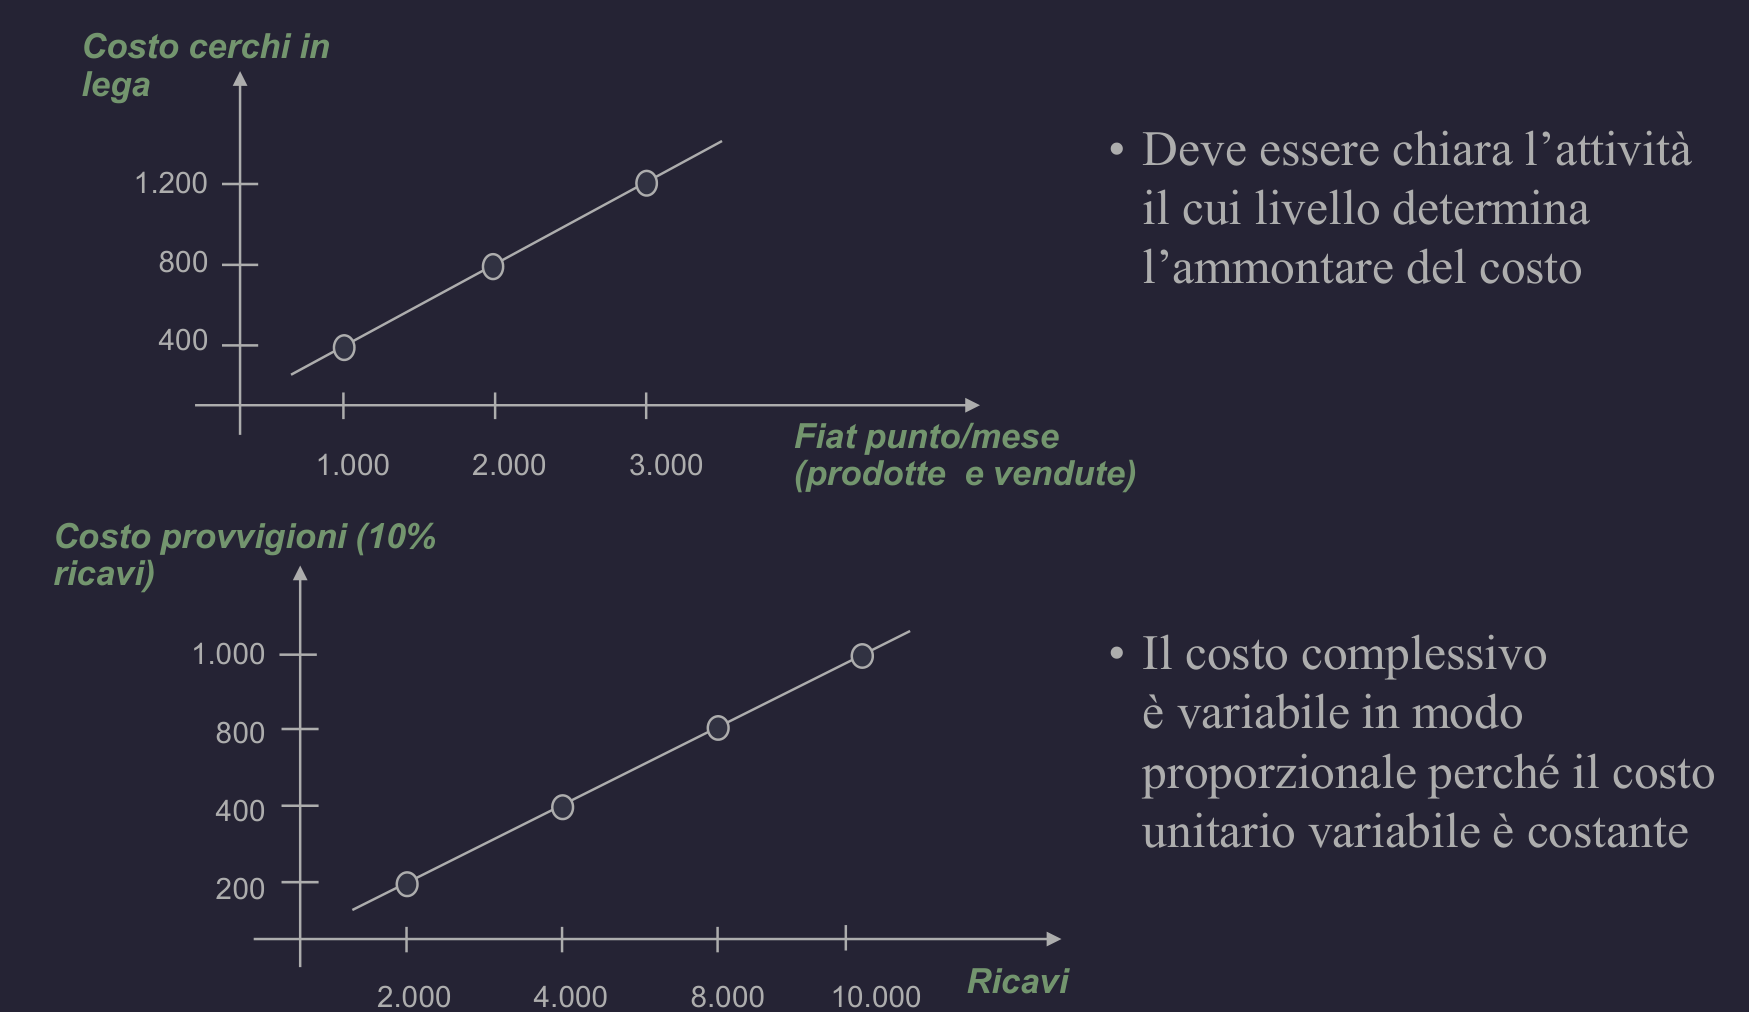
\includegraphics[scale=0.3]{Image/Costi_Var.png}
\end{center}


\subsubsection{I costi fissi}
I \textit{costi fissi} sono quelli il cui ammontare complessivo non varia al modificarsi del livello di output. Possono comunque modificarsi nel tempo, ma non a seguito di cambiamenti del livello di attività in un determinato periodo di tempo; possono variare ad esempio in seguito all'assunzione di nuovi professionisti.
\vspace*{0.1cm}\\
I costi fissi si dividono in \underline{costi impegnati} e \textbf{cosi discrezionali}.
\vspace{0.2cm}\\


\subsubsection*{I costi impegnati}
I costi impegnati sono costi necessari a rendere disponibile una certa capacità produttiva o di servizio. Esempi di costi impegnati sono: ammortamenti, i canoni di locazione, gli stipendi dei dirigenti.
\vspace*{0.1cm}\\
I costi impegnati riflettono l'ammontare della \underline{capacità acquistata} e \underline{resa disponibile} piuttosto che la capacità effettivamente utilizzata, e si riferiscono a risorse che vengono adeguate al fabbisogno solo nel medio-lungo periodo. È facile evidenziare come i costi impegnati non possono essere radicalmente ridimensionati senza compromettere le prestazioni economiche dell'azienda.
\vspace*{0.1cm}\\


\subsubsection*{I costi discrezionali}
I \underline{costi discrezionali} sono risultati di decisioni che il management rinnova periodicamente in fase di programmazione delle attività, e vengono stabiliti in base ai volumi di attività stimati. Ne sono un esempio le azioni promozionali, la formazione del personale, la ricerca e sviluppo. Sono relativi a risorse che possono essere adeguate al fabbisogno in relazione a lassi di tempo brevi.


\subsubsection{I costi semi-variabili}
I \underline{costi semi-variabili} sono costi che variano in funzione del volume o del livello di attività, ma meno rapidamente. Sono una combinazione di costi variabili e costi fissi, infatti vengono anche chiamati \underline{costi misti}. Un esempio di costo semi-variabile è il costo dell'energia.

\begin{center}
    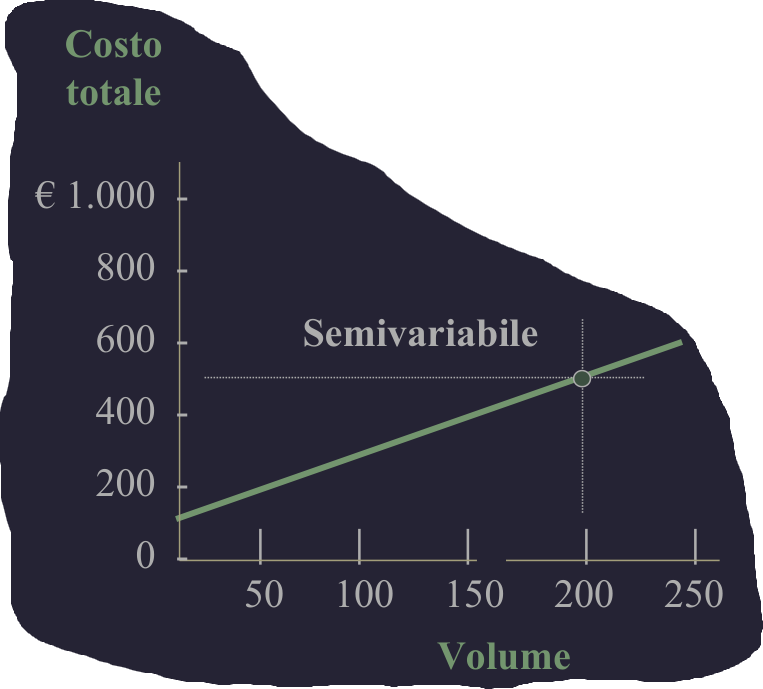
\includegraphics[scale=0.3]{Image/Costi_SemiVar_1.png}
    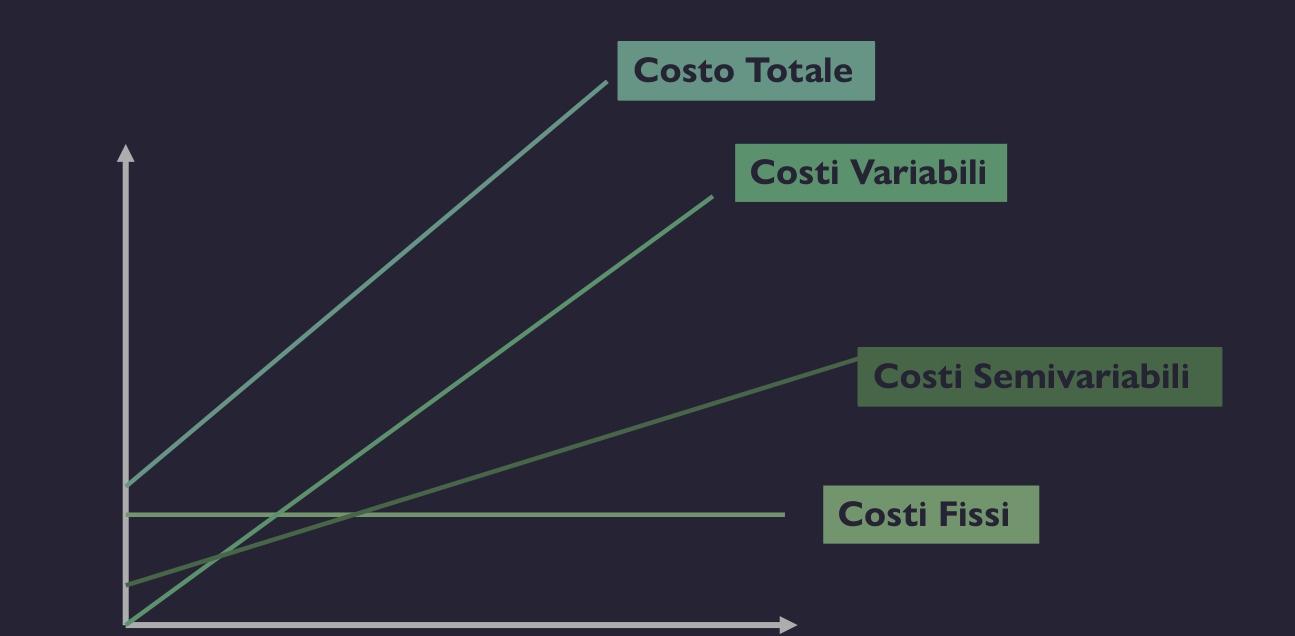
\includegraphics[scale=0.3]{Image/Costi_SemiVar_2.png}
\end{center}
\[
    \T{Costo totale} = \T{Costi fissi} + (\T{Costi variabili} \times \T{Volume}) + (\T{Costi semi-variabili} \times \T{Volume})
\]


\subsubsection*{Esempio}
L'azienda Rinfresca Gola produce gelato a un costo fisso annuale pari a 5.000 €. I Costi variabili sono pari a 10 € per Kg e i costi semi-variabili hanno una quota di costo fisso di 3.000 €, che rimane inalterata nel periodo considerato, e un costo variabile unitario pari a 4 €. Quale è il costo totale per produrre 1.000 kg di gelato?
\[
    \T{Costo totale} = 5.000 + (10 \times 1.000) + (3.000 +(4 \times 1.000)) = 22.000
\]


\subsection{Relazione tra costi unitari e volume}
Il costo medio unitario si comporta in maniera diversa dal costo totale: rimane costante se il costo è solo variabile, mentre diminuisce se cresce il volume (economia di scala)
\[
    \T{Costo Unitario} = \frac{\T{CF} + \T{CV} \times \T{Volume}}{\T{Volume}}
\]
Ad esempio, per l'azienda Congela Gola, la curva del costo unitario è descritta dal seguente grafico:
\begin{center}
    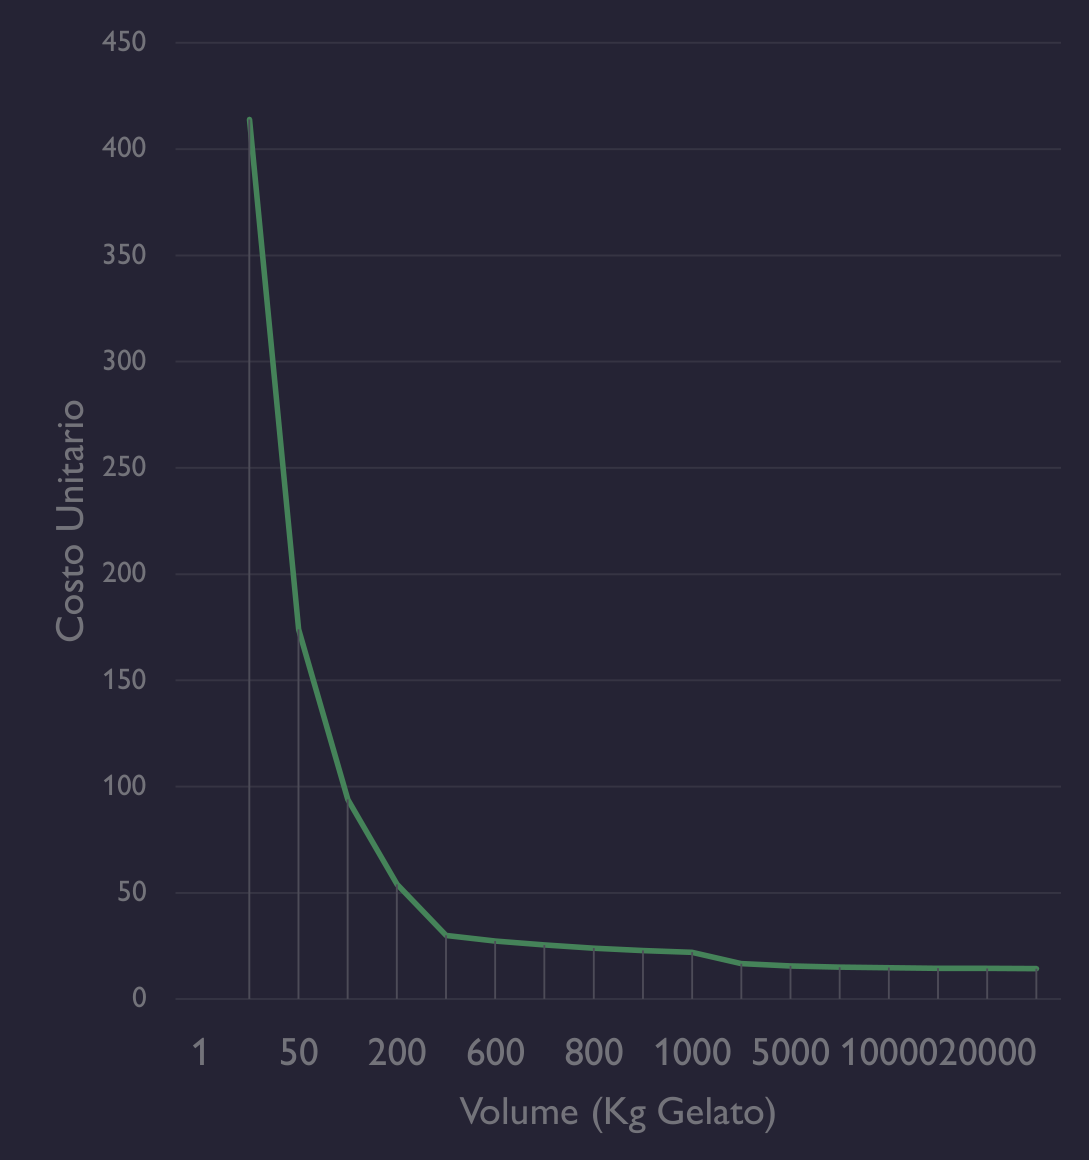
\includegraphics[scale=0.3]{Image/CostoUni_1.png}
\end{center}
\[
    \T{Costo Unitario} = \frac{(5.000 \T{\euro} + 3.000 \T{\euro}) + 14 \times \T{Volume}}{\T{Volume}}
\]



\subsubsection{Intervallo di rilevanza}
\begin{center}
    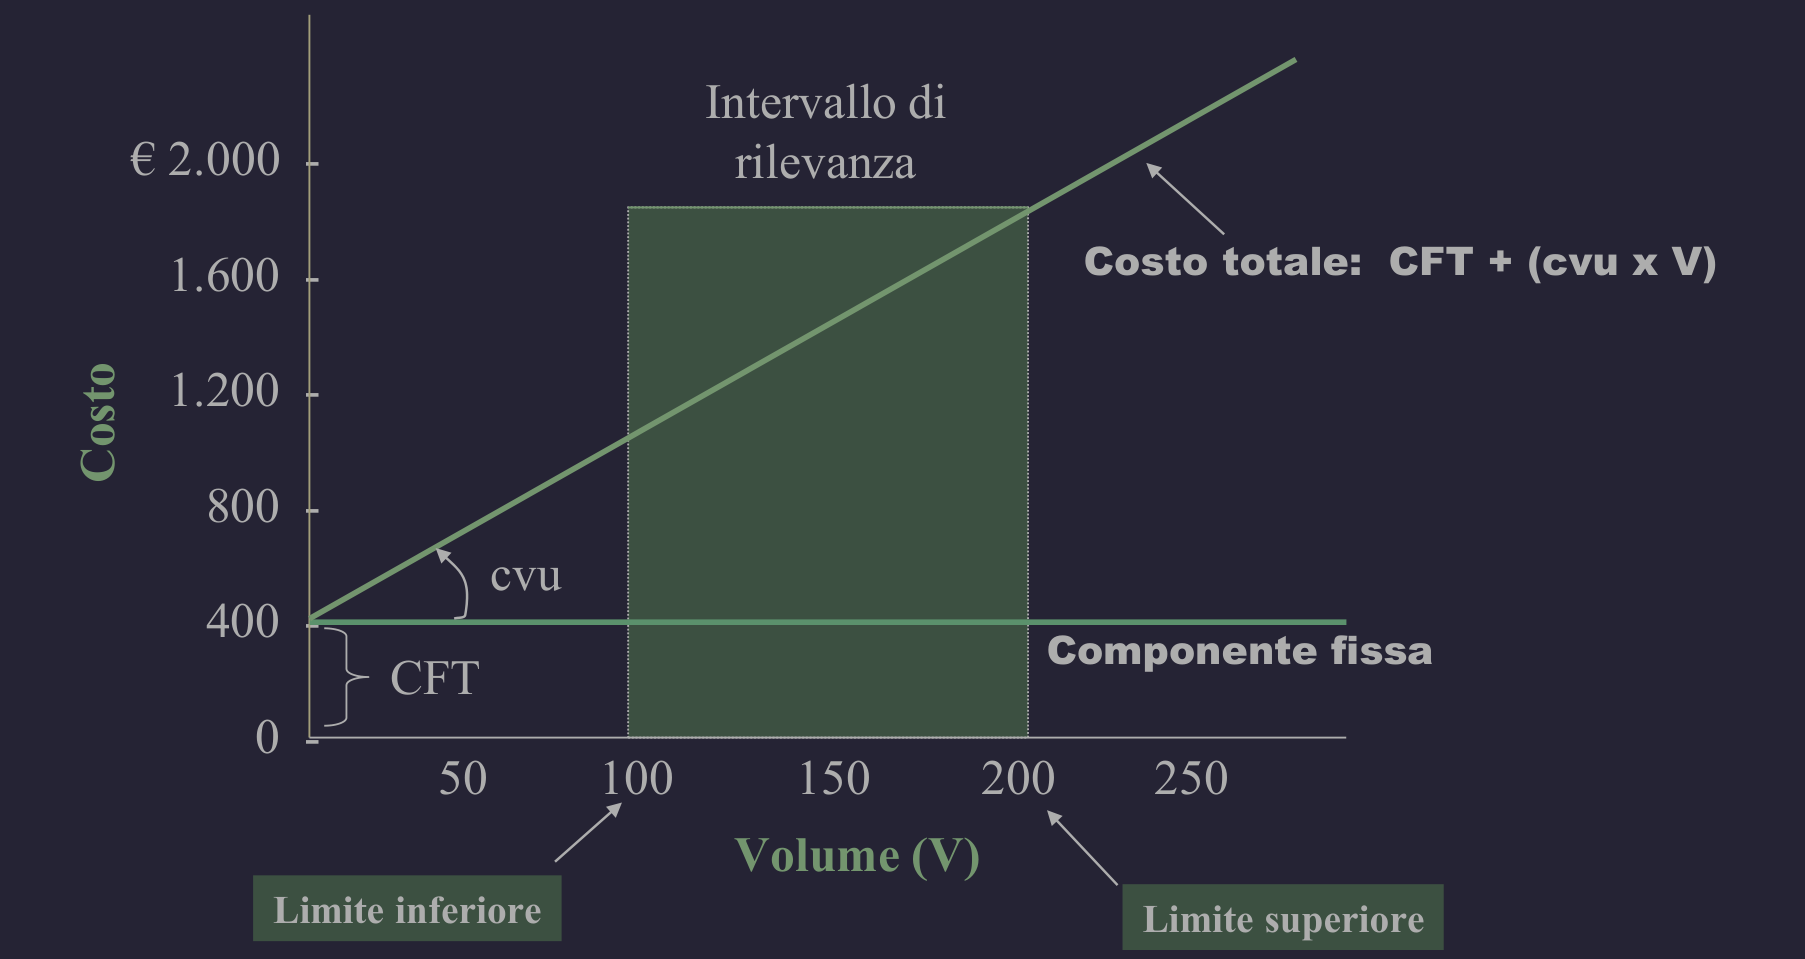
\includegraphics[scale=0.3]{Image/CostoUni_2.png}
\end{center}
L'\underline{intervallo di rilevanza} è l'intervallo di attività o di volume all'interno del quale si suppone valida una specifica relazione fra il livello di attività/volume e il costo.
\vspace*{0.2cm}\\
Se i costi fissi annuali di un reparto che assembla biciclette sono 94.500€ e rimanessero gli stessi all'interno del volume di produzione 1.000-5.000 biciclette, allora l'intervallo da 1.000€ a 5.000€ biciclette sarebbe l'intervallo di rilevanza di costo fisso totale di 94.500€.\\
Se la domanda annuale di biciclette aumentasse e l'impresa dovesse assemblare più di 5.000 biciclette, allora dovrebbe disporre di maggiori risorse impegnate sostenendo più alti costi fissi totali.


\subsubsection{Periodo temporale di rilevanza}
L'ammontare dei costi che possono essere adeguati al fabbisogno dipende dall' \textit{intervallo temporale} al quale si riferisce la valutazione.
\begin{itemize}
    \item intervallo breve: quasi tutti i costi non sono modificabili (sono impegnati);
    \item intervallo medio/lungo: molti costi sono non modificabili, ma molti sono flessibili (adattabili)
    \item intervallo lungo: l'ammontare di quasi tutti i costi è flessibile al fabbisogno
\end{itemize}


\subsubsection{Contesto ambientale}
Il \textit{contesto ambientale} comprende altre cause diverse dal volume che possono incidere sull'ammontare dei costi, ad esempio:
\begin{itemize}
    \item inflazione dei prezzi dei materiali;
    \item cambiamenti della tecnologia e dei processi produttivi
    \item cambiamenti dei contratti
    \item \dots
\end{itemize}


\subsection{Costi a gradino}
Alcuni elementi di costo possono variare \textit{a gradino} con i livelli di attività. Sono costi che si riferiscono al consumo di \textbf{risorse acquisibili solo in blocchi minimi}, in quantità discrete. Ad esempio l'aggiunta di un coordinatore ogni 10 impiegati, nel cui caso il costo additivo è effettivamente lo stipendio del nuovo dipendente.
\begin{center}
    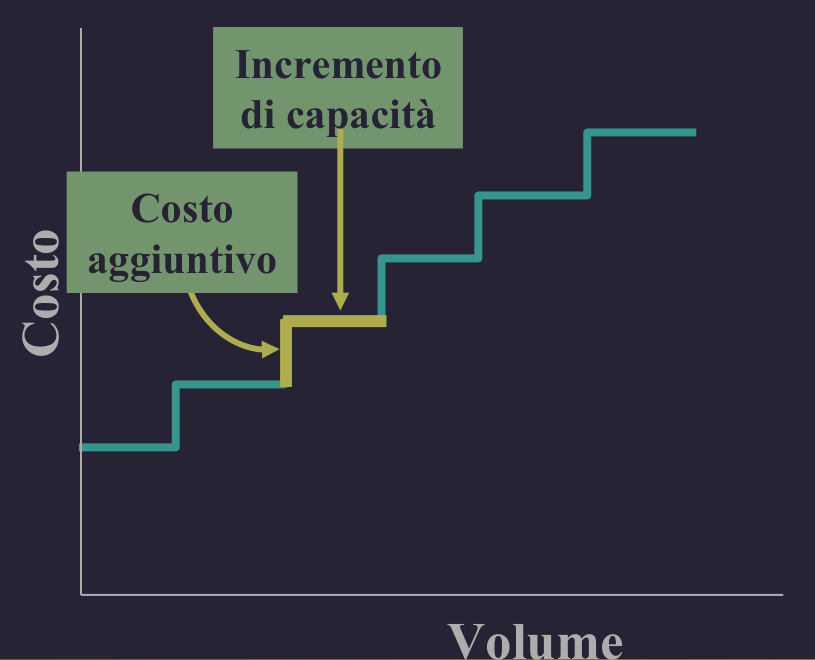
\includegraphics[scale=0.3]{Image/CostiGradino_1.png}
\end{center}


\subsubsection{Costi viscosi (sticky)}
I \textit{costi viscosi} sono dei costi che normalmente sono ritenuti variabili anche quando il volume dell'attività non si riduce. Essi si contraggono meno rapidamente, quando il volume diminuisce, di quanto crescano quando il volume aumenta.
\begin{center}
    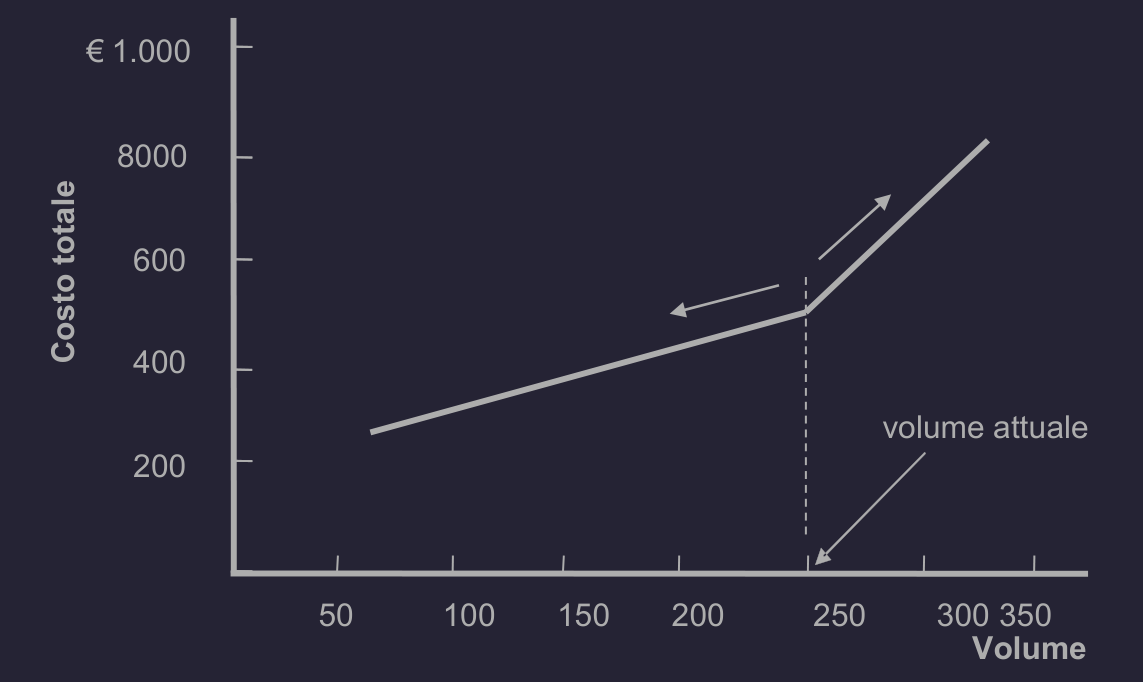
\includegraphics[scale=0.3]{Image/Costi_Viscosi_1.png}
\end{center}



\subsection{Stima della relazione costo-volume}
Si possono utilizzare diversi metodi per la stima della relazione esistente tra costi e volumi, i due principali sono:
\begin{enumerate}
    \item \underline{Valutazione soggettiva} (metodo conto per conto): I costi sono definiti soggettivamente,
    attraverso il giudizio di chi compie la valutazione. Il criterio è appropriato ove i dati storici non
    siano rilevanti o disponibili o quando non vale la pena applicare metodi più onerosi in termini
    di tempi e denaro;
    \item \underline{Regressione lineare}: Si utilizza la tecnica metodo dei minimi quadrati e fornisce direttamente i
    valore corrispondenti al totale dei costi fissi e al costo unitario. Tramite questo metodo viene
    tracciata una linea retta che approssima statisticamente una serie di punti rappresentanti il
    costo totale consuntivo in relazione a diversi volumi.
\end{enumerate}


\subsubsection{Regressione lineare e problemi con le stime statistiche}
\begin{center}
    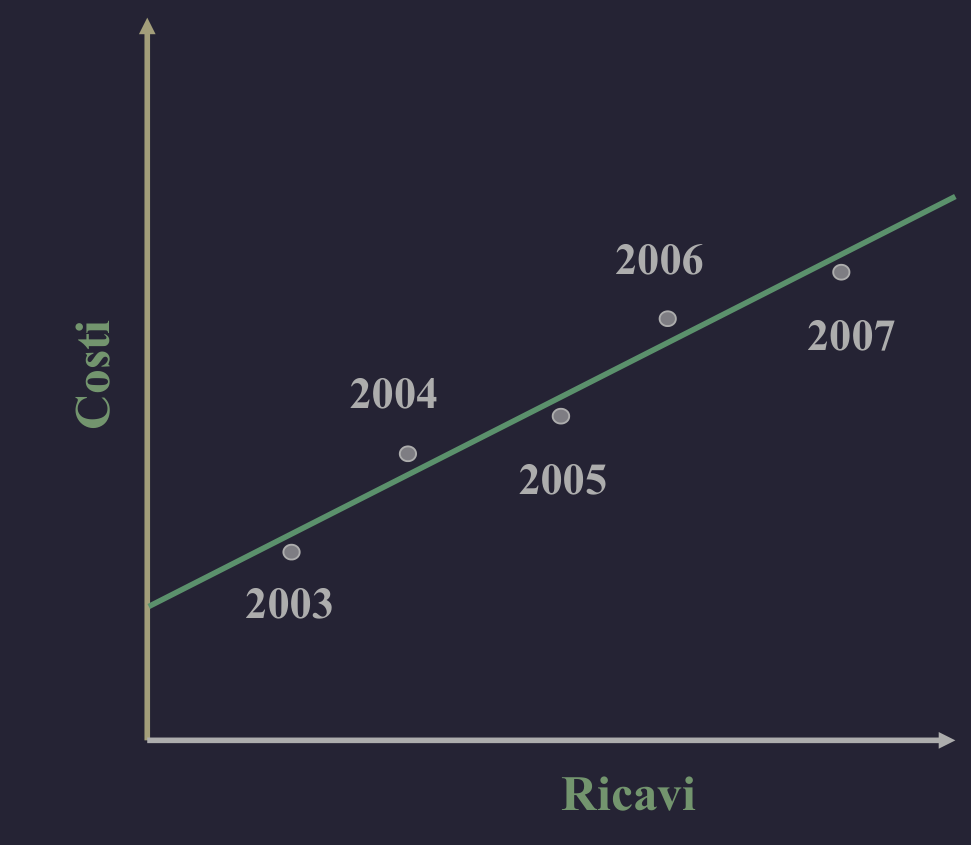
\includegraphics[scale=0.3]{Image/RegressioneLin_1.png}
\end{center}
Utilizzare la regressione lineare può avere dei problemi:
\begin{itemize}
    \item si rilevano relazioni passate tra costi e volume, ma le ipotesi operative future potrebbero essere diverse;
    \item i ricavi potrebbero non essere una misura adeguata del volume; la retta potrebbe mostrare l'effetto di prezzi crescenti (ad esempio per causa dell'inflazione) e non la relazione tra costi e volumi;
    \item il grafico ci potrebbe portare a pensare che i costi, all'interno di un periodo siano semi-variabili, ma nella realtà non è così
    \begin{center}
        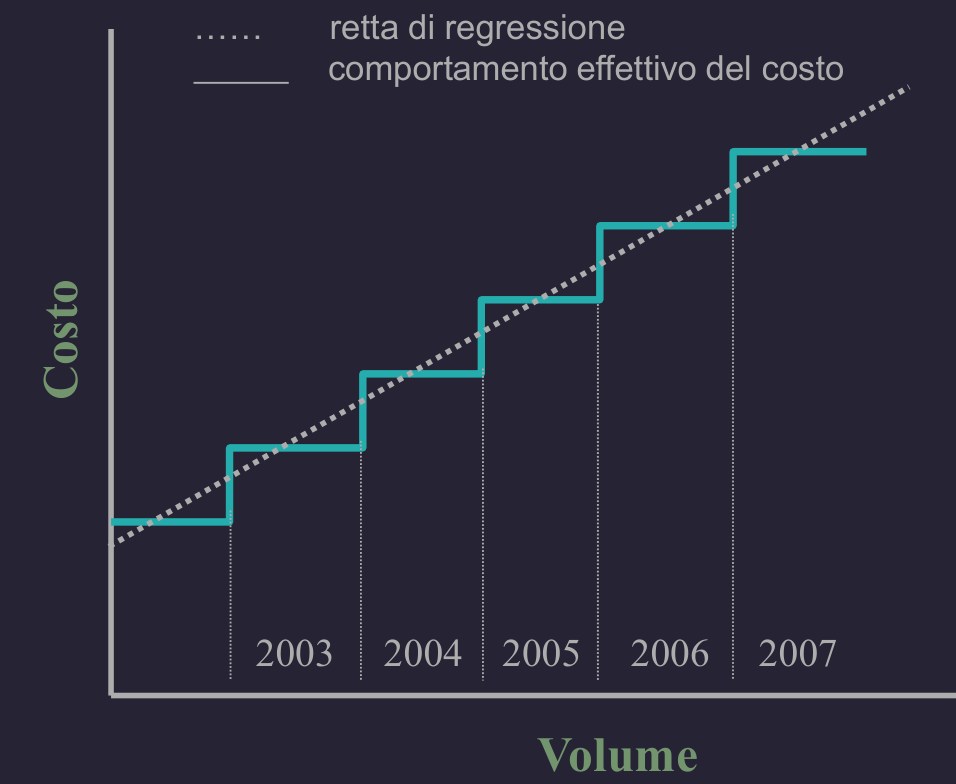
\includegraphics[scale=0.3]{Image/RegressioneLin_2.png}
    \end{center}

    \item non si devono trarre conclusioni sul comportamento dei costi nel breve periodo da un'analisi di regressione che si riferisce al lungo periodo.
\end{itemize}


\subsubsection{Misurare il volume}
Analizzare la relazione tra costo e volume di un'azienda che produce tanti prodotti può portare diverse sfide. In questo caso il volume non è l'unità di misura più affidabile e adeguata, sarebbe meglio utilizzare le ore di manodopera diretta, le ore di macchina, i ricavi o altre unità di misura quantitative omogenee (tonnellate, metri cubi, \dots). In generale bisogna scegliere l'unità di misura che riflette al meglio le condizioni che determinano la variazione dei costi.\\
Per capire quale unità usare si prova a rispondere a due domande:
\begin{enumerate}
    \item la misura da avere fa riferimento agli input o agli output?
    \item la misura deve essere espressa in termini monetari o non monetari?
\end{enumerate}









\section{Relazioni fra reddito e volume}
\subsection{Diagramma del profitto}
Il \textit{diagramma del profitto} mostra la relazione attesa tra i \textbf{ricavi} e i \textbf{costi totali} al variare del \textbf{volume} di output, per questo è chiamato anche diagramma costo-volume-profitto. Può essere costruito sia per l'impresa nel suo complesso sia per specifici segmenti di business, come un prodotto, una linea di prodotti o una divisione. Il volume di output può essere misurato come numero di unità prodotte e vendute o anche in termini di ricavi realizzati.
Di seguito si riportano il diagramma volume-ricavi (a sinistra), il diagramma costo-volume (a destra) e il diagramma costo-volume-profitto (in basso)
\begin{center}
    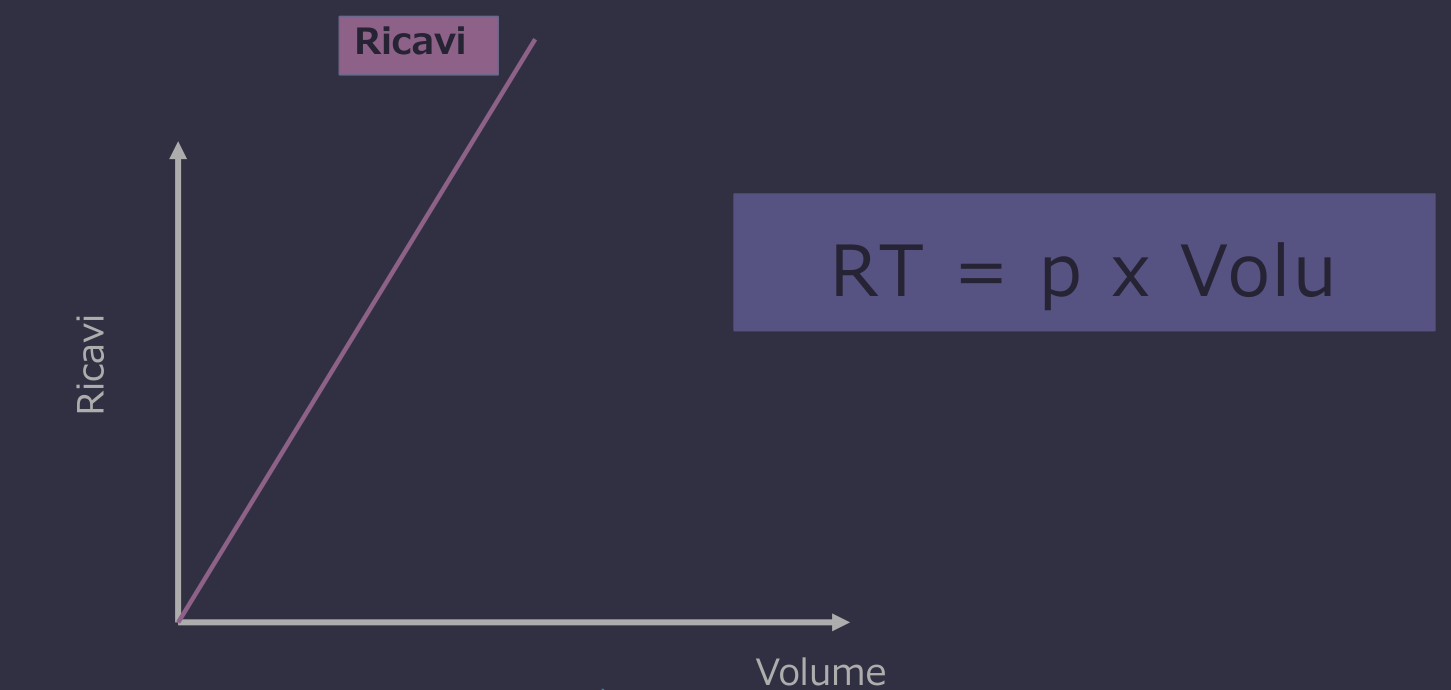
\includegraphics[scale=0.25]{Image/DiagrammaProfitto_1.png}
    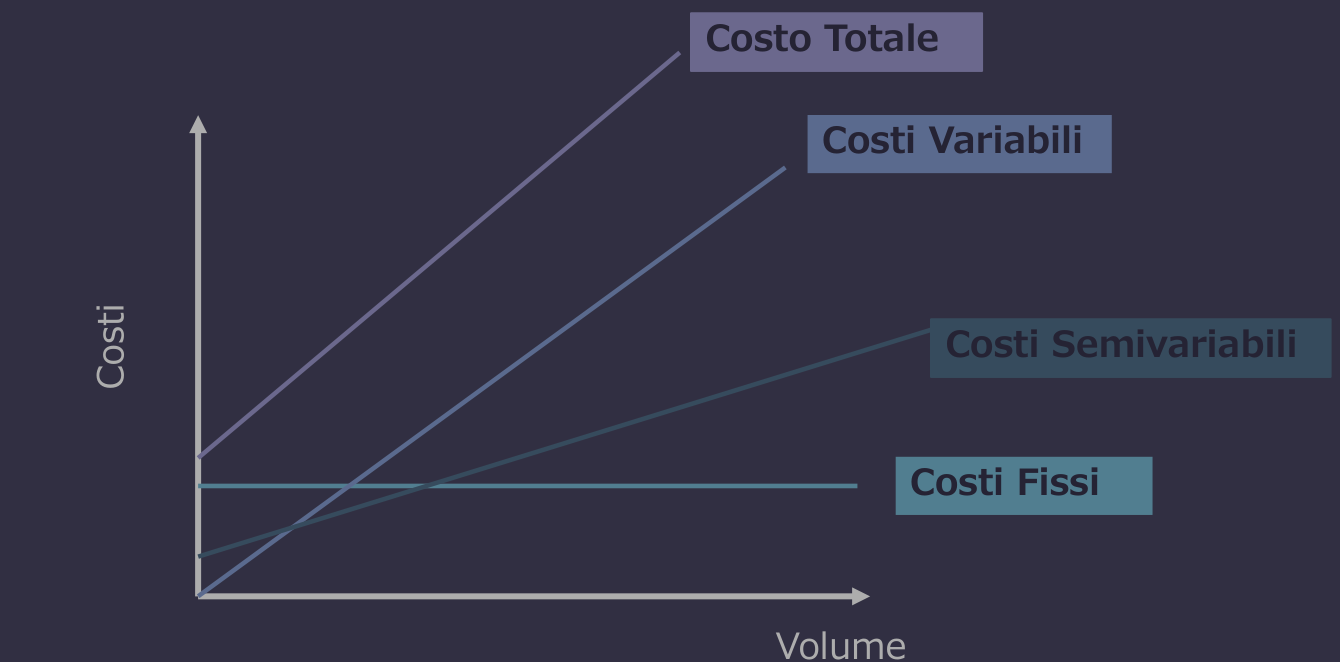
\includegraphics[scale=0.25]{Image/DiagrammaProfitto_2.png}
    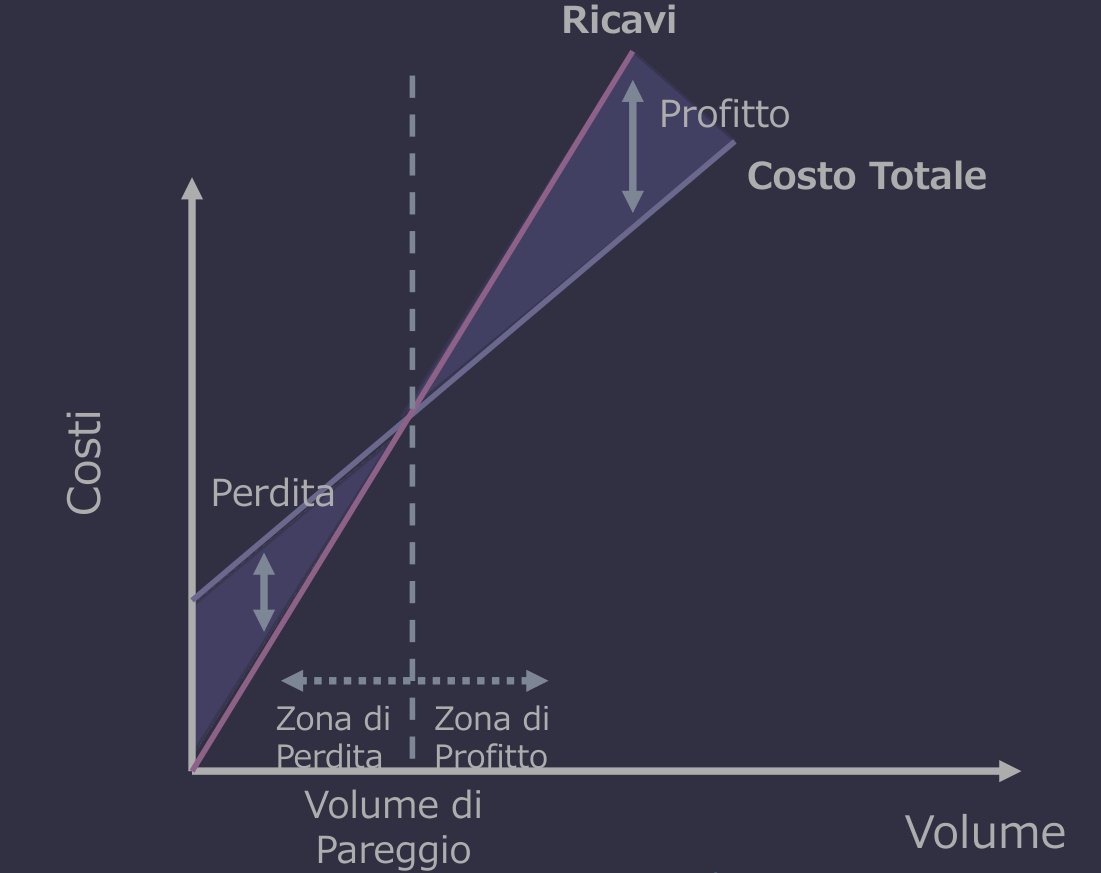
\includegraphics[scale=0.3]{Image/DiagrammaProfitto_3.png}
\end{center}
Il diagramma del profitto è uno strumento utile per capire il processo di formazione del reddito in funzione delle quantità vendute o dei ricavi.\\
Il volume di pareggio o punto di pareggio (\textit{break-even point}) è il punto dove il reddito è pari a zero, dunque i costi totali son uguali ai ricavi totali.
\vspace*{0.1cm}\\
Il volume di  pareggio è calcolato dividendo i costi fissi totali per la differenza tra il prezzo di vendita unitario e il costo variabile unitario.
\[
    \T{Vol} = \frac{\T{CF}}{(\T{p}_u - \T{CV}_u)}
\]
L'equazione di costo di produzione dell'azienda Rinfresca Gola per Kg, determinata nella lezione scorsa, è:
\[
    \T{CT} = 8.000 \T{\euro} + (14 \T{\euro} \times \T{Vol})
\]
e ha un prezzo di vendita pari a 30 euro per Kg, quindi il suo punto di pareggio è
\[
    \T{Vol(Kg)} = \frac{8.000 \T{\euro}}{(30 \T{\euro}-14\T{\euro})} = 500 \T{\euro}
\]







\subsection{Margine di contribuzione}
Equazione del profitto:
\[
    \T{PR} = \underbrace{(\T{p}_u - \T{CV}_u)}_{\color{synthwave_text} \substack{\text{margine di} \\ \text{contribuzione}}} \times \T{Vol} - \T{CF}
\]
La differenza tra il prezzo unitario e il costo variabile unitario è chiamata \textit{margine di contribuzione}, che rimane costante nell'intervallo di rilevanza; esso permetto di calcolare il profitto medio unitario per volume venduto. Il suo impiego si rivela utile per esprimere in modo semplice e sintetico la relazione tra ricavi e costi in funzione del volume.
\begin{align*}
    \T{Equazione }&\T{del punto di pareggio in volume} & \T{Equazione }&\T{del punto di pareggio in ricavi}\\
    \T{Vol} =& \dfrac{\T{CF}}{\T{Margine di contribuzione}} & \T{Vol} =& \dfrac{\T{CF}}{\T{Margine di contribuzione }\%}
\end{align*}


\subsubsection{Margine di contribuzione percentuale}
Il \textit{margine di contribuzione percentuale} rappresenta il percentuale tra il margine di contribuzione e il prezzo di vendita, e sostanzialmente ci dice quanti euro di contribuzione vengono prodotti per ciascun euro di ricavo; rappresenta l'effetto economico derivante da aumenti di ricavo. 
\vspace*{0.2cm}\\
Di seguito si riporta un disegno che potrebbe rendere più chiaro il concetto
\begin{center}
    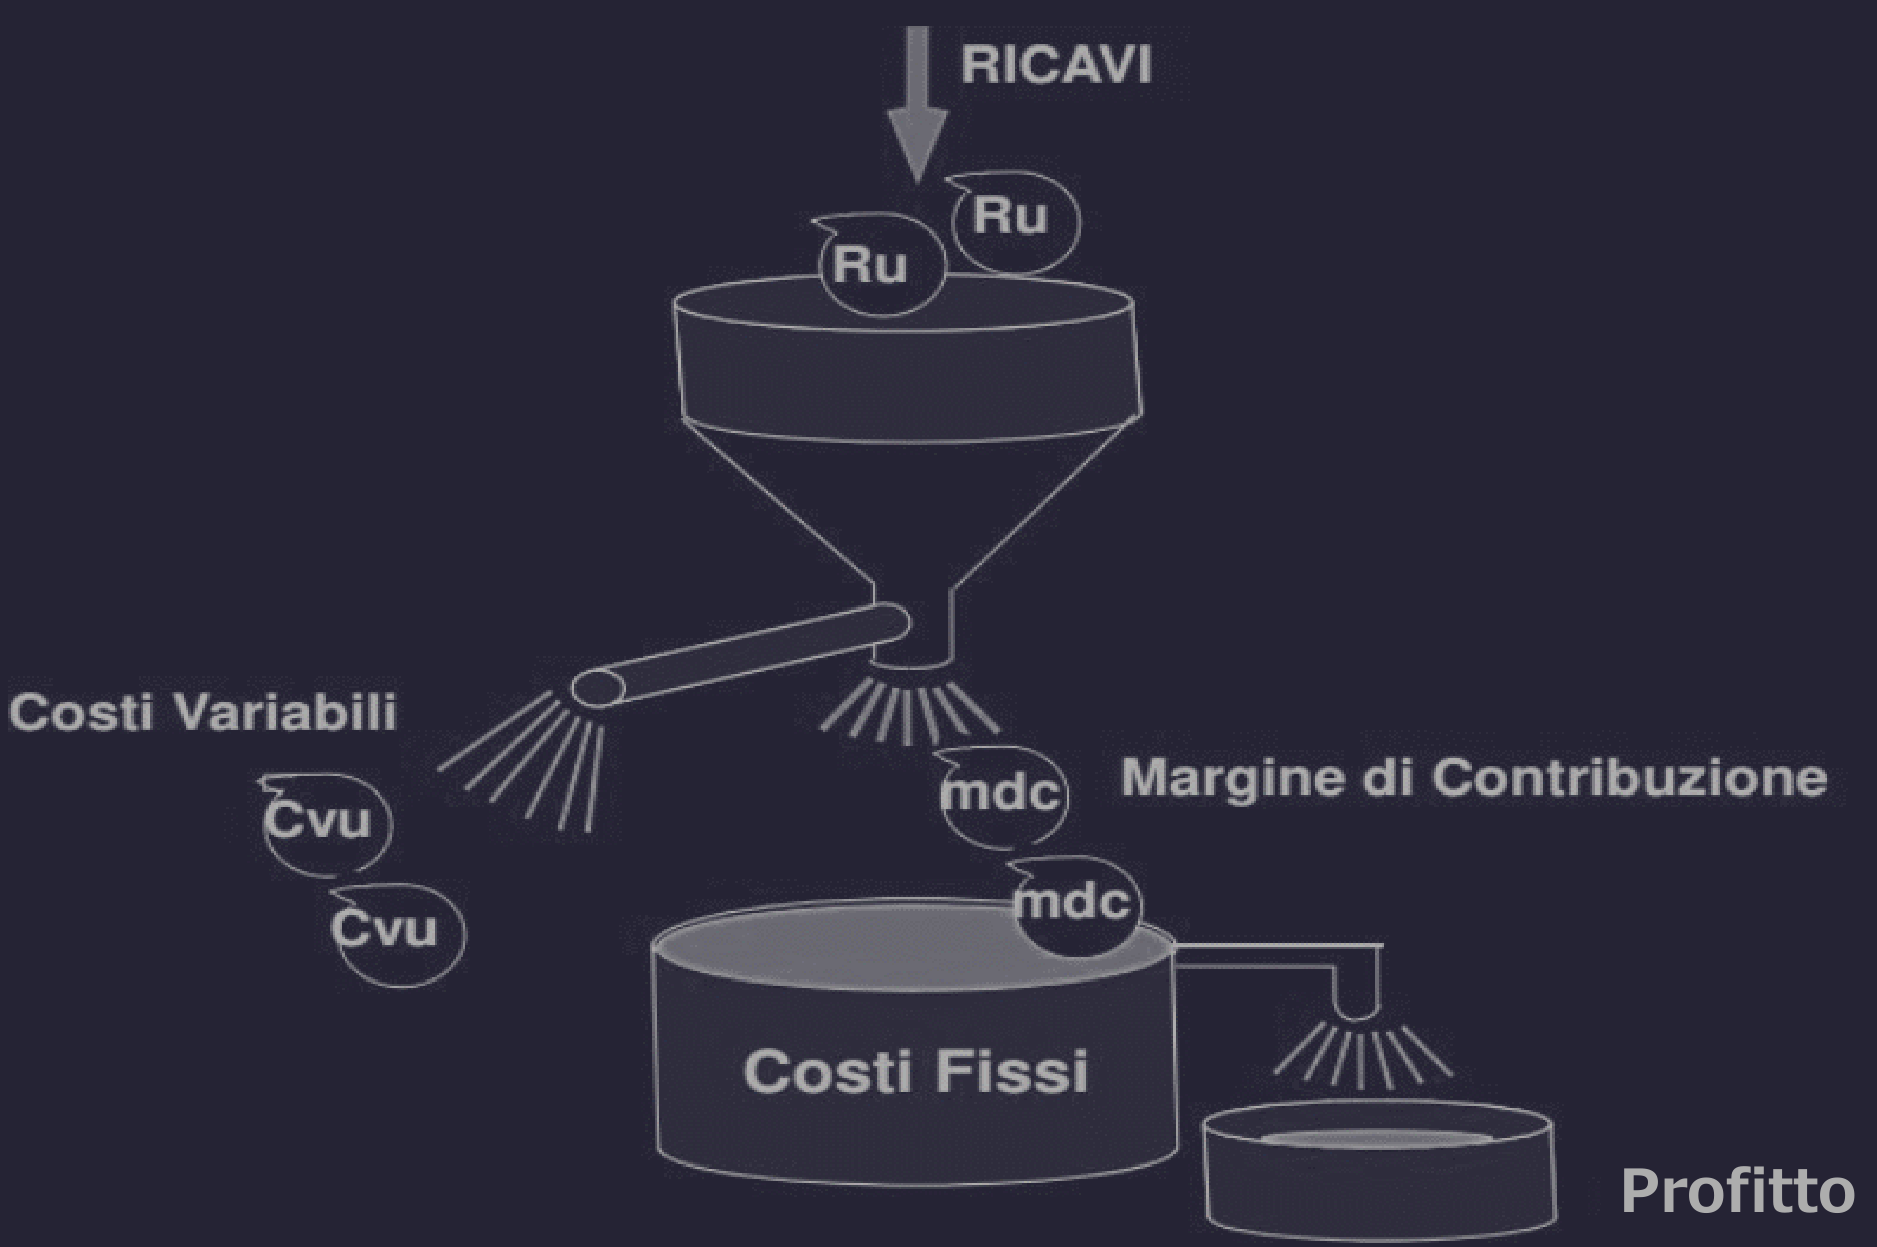
\includegraphics[scale=0.25]{Image/MargineContr_1.png}
\end{center}


\subsubsection{Esempio}
Analizziamo i dati dell'azienda Rinfresca Gola:
\begin{itemize}
    \item prezzo vendita = 30 \euro per Kg
    \item costi fissi = 8.000 \euro
    \item costi variabili = 14 \euro per Kg
    \item margine di contribuzione = $(30 - 14) = 16$
    \item margine di contribuzione \% = $16/30 = 53,33 \%$
    \item punto di pareggio = $8.000 \T{\euro}/16 \T{\euro} = 500 \T{\euro}$ 
\end{itemize}
\begin{center}
    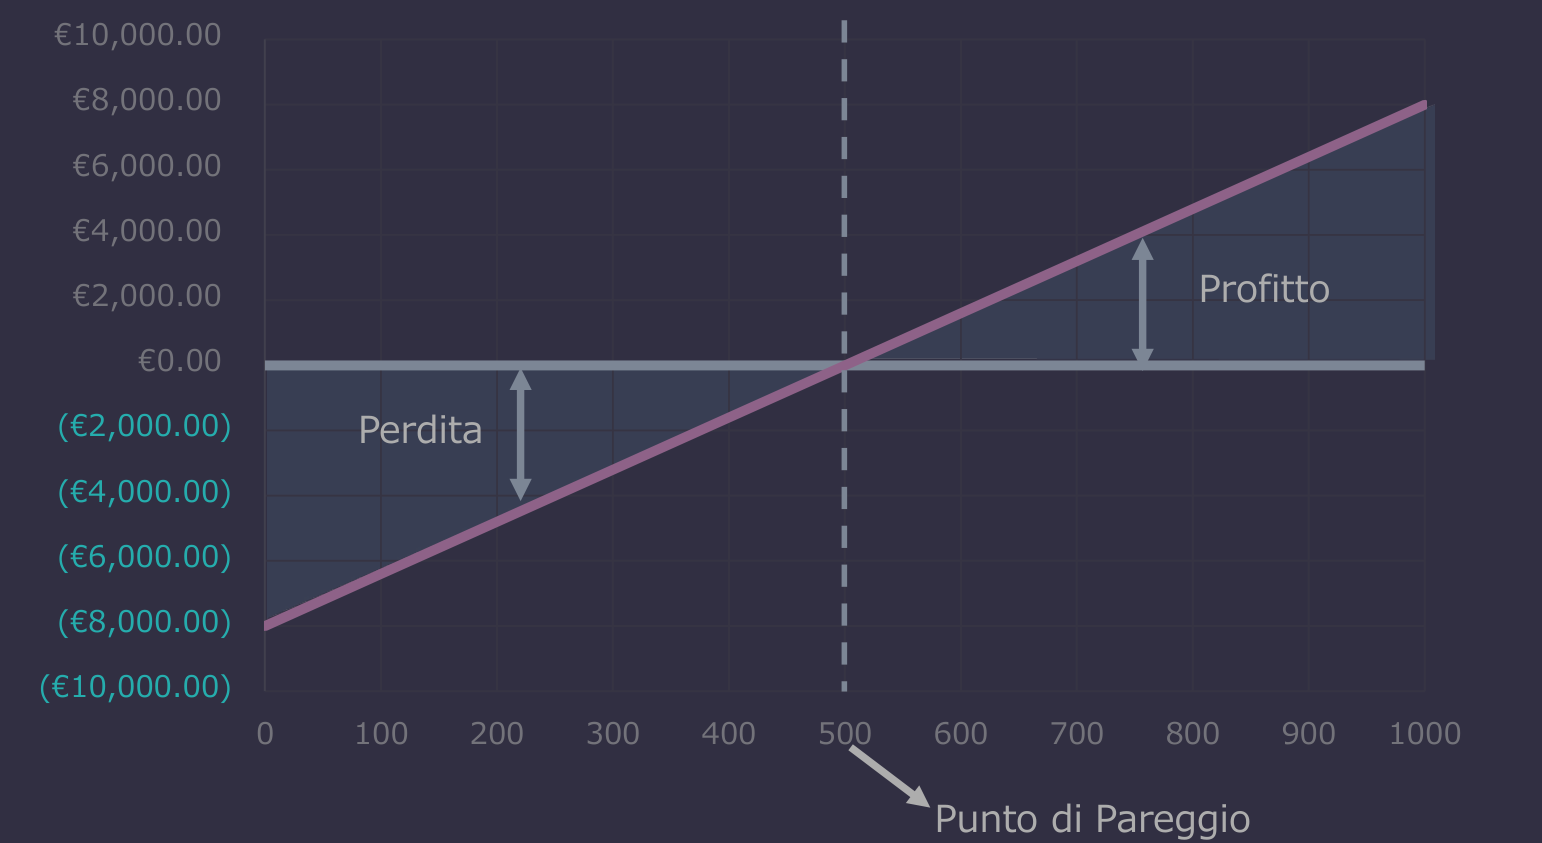
\includegraphics[scale=0.3]{Image/MargineContr_2.png}
\end{center}



\subsection{Come migliorare la prestazione in termini di profitto}
Esistono quattro principali determinanti per accrescere il reddito di un'azienda monoprodotto:
\begin{enumerate}
    \item aumentare il prezzo unitario di vendita
    \item ridurre il costo variabile unitario
    \item ridurre i costi fissi totali
    \item aumentare il volume
\end{enumerate}
Ad esempio
\begin{center}
    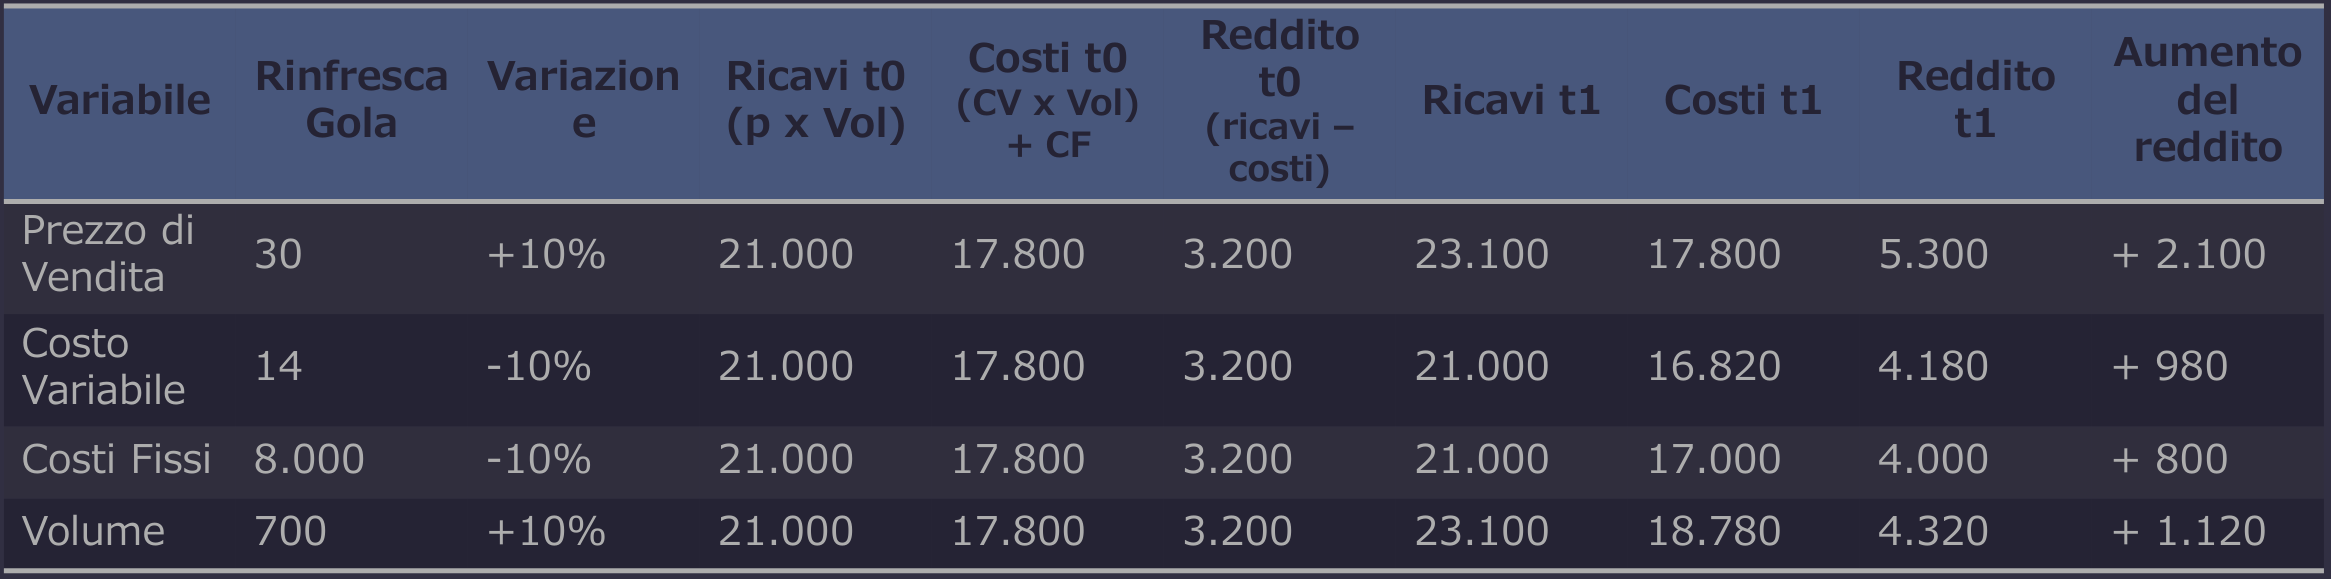
\includegraphics[scale=0.3]{Image/PrestazioniProf_1.png}
\end{center}


\section{I costi pieni e il loro impiego}
\subsection{Il concetto di costo}
Il \textit{costo} quantifica l'impiego di risorse (la misura del costo è espressa in termini monetari).
\begin{center}
    Il costo è la valorizzazione monetaria delle risorse consumate (da consumarsi) per un qualche scopo
\end{center}
I possibili oggetti del costo sono:\
\begin{center}
  \begin{tabular}{|r|l|}
    \hline
    Prodotto & una giacca, un PC, un tornio, un portale, un Panda 4X4, ...\\
    \hline 
    Servizio & un volo da Bologna a Catania, l'emissione di un certificato, ... \\
    \hline 
    Linea di Prodotto & Rolex Datejust, una linea di biscotti MB, \dots \\ 
    \hline 
    Marchio & Emporio Armani, Maserati, Nike, \dots \\
    \hline 
    Agente & Andrea Rossi, \dots \\
    \hline 
    Canale & un insieme omogeneo di punti vendita (al dettaglio o all'ingrosso)\\
    \hline
    Progetto & un aeromobile, un principio attivo, un progetto BPR, ... \\
    \hline
    Cliente & una catena distributiva, un'impresa, un PV, una persona, ... \\
    \hline 
    Attività & un test di controllo di qualità, la selezione di fornitori, ... \\
    \hline
    Funzione & riscaldare i sedili, stampare un foglio su due lati, ... \\ 
    \hline
    Unità organizzativa & la produzione, il commerciale, la R\&S \\
    \hline 
 \end{tabular}  
\end{center}



\subsection{Il costo pieno}
Il \textit{costo pieno} comprende tutte le risorse utilizzate per un determinato oggetto di costo.\\
In determinate circostanze il costo pieno è semplice da valutare (il prezzo pagato), in altre potrebbe richiedere un sistema di rilevazioni complesso. Il costo pieno è la somma di \textit{costi diretti} e di una quota equa di \textit{costi indiretti}.



\subsubsection{Costi diretti e costi indiretti}
I termini diretto e indiretto hanno a che fare con il \textbf{trattamento contabile} dei costi; la classificazione è basata sull'oggetto del costo:
\begin{itemize}
    \item \textbf{Costi diretti:} sono assegnati in modo oggettivo e vengono attribuiti all'oggetto;
    \item  \textbf{Costi indiretti:} sono assegnati utilizzando criteri di ripartizione soggettivi, essi non sono attribuiti all'oggetto ma allocati.
\end{itemize}
Ad esempio, se l'oggetto del costo è un lotto di jeans:
\begin{itemize}
    \item i costi diretti sono: il tessuto utilizzato e le ora di manodopera usata per trasformare il tessuto originale in pantaloni
    \item i costi indiretti sono: lo stipendio dei direttori, i costi d'assicurazione dello stabilimento e i costi del dipartimento acquisti 
\end{itemize}


\subsubsection{Costi speciali e costi comuni}
\begin{itemize}
    \item \textbf{Costi speciali:} elementi di costo “oggettivamente” riconducibili a un oggetto del costo
    (possono essere contabilmente trattati sia come diretti che come indiretti);
    \item \textbf{Costi comuni:} Elementi di costo causati congiuntamente da due o più oggetti del costo e dunque non riconducibili oggettivamente ad alcuno di essi singolarmente; i costi comuni sono allocati ai prodotti utilizzando criteri necessariamente soggettivi di ripartizione, infatti sono \textbf{indiretti}.
\end{itemize}



\subsection{Il costo del prodotto}
Il concetto di costo e il principio di competenza stabiliscono come suddividere i costi complessivi di un periodo tra quelli da assegnare al \textit{costo del venduto} e quelli da assegnare alle rimanenze finali. Non forniscono però alcuna indicazione du come calcolare il costo dei singolo prodotti.\\
Ad esempio è possibile allocare i costi indiretti in proporzione alle ore di manodopera o alle ore impianto, sebbene il risultato dul costo del prodotto possa essere significativamente diverso.


\subsubsection{Gli elementi di costo del prodotto}
Il sistema che rileva e rappresenta i costi del prodotto è denominato \textbf{contabilità industriale} o \textbf{sistema di contabilità dei costi di prodotto}.
\vspace*{0.2cm}\\
Glie elementi di costo del prodotto sono:
\begin{itemize}
    \item \textbf{materiali diretti:} hanno a che fare con qualsiasi elemento o componente  che dia acquistato e utilizzato per realizzare i prodotti finiti;
    \item \textbf{manodopera diretta:} è la quantità di manodopera riconducibile in maniera oggettiva ed economicamente conveniente a un oggetto del costo, valorizzata al costo orario del lavoro;
    \item \textbf{costi indiretti di produzione:} tutti i costi di produzione diversi dai costi diretti (overhead costs). Sono generalmente costi fissi, tendono dunque a mantenersi complessivamente costanti nel tempo; tra questi costi figurano:
    \begin{itemize}
        \item manutenzione impianti generali
        \item logistica interna
        \item programmazione della produzione
        \item riscaldamento stabilimento
        \item illuminazione stabilimento
        \item pulizie stabilimento
        \item materiali di consumo
    \end{itemize}
\end{itemize}
\begin{center}
    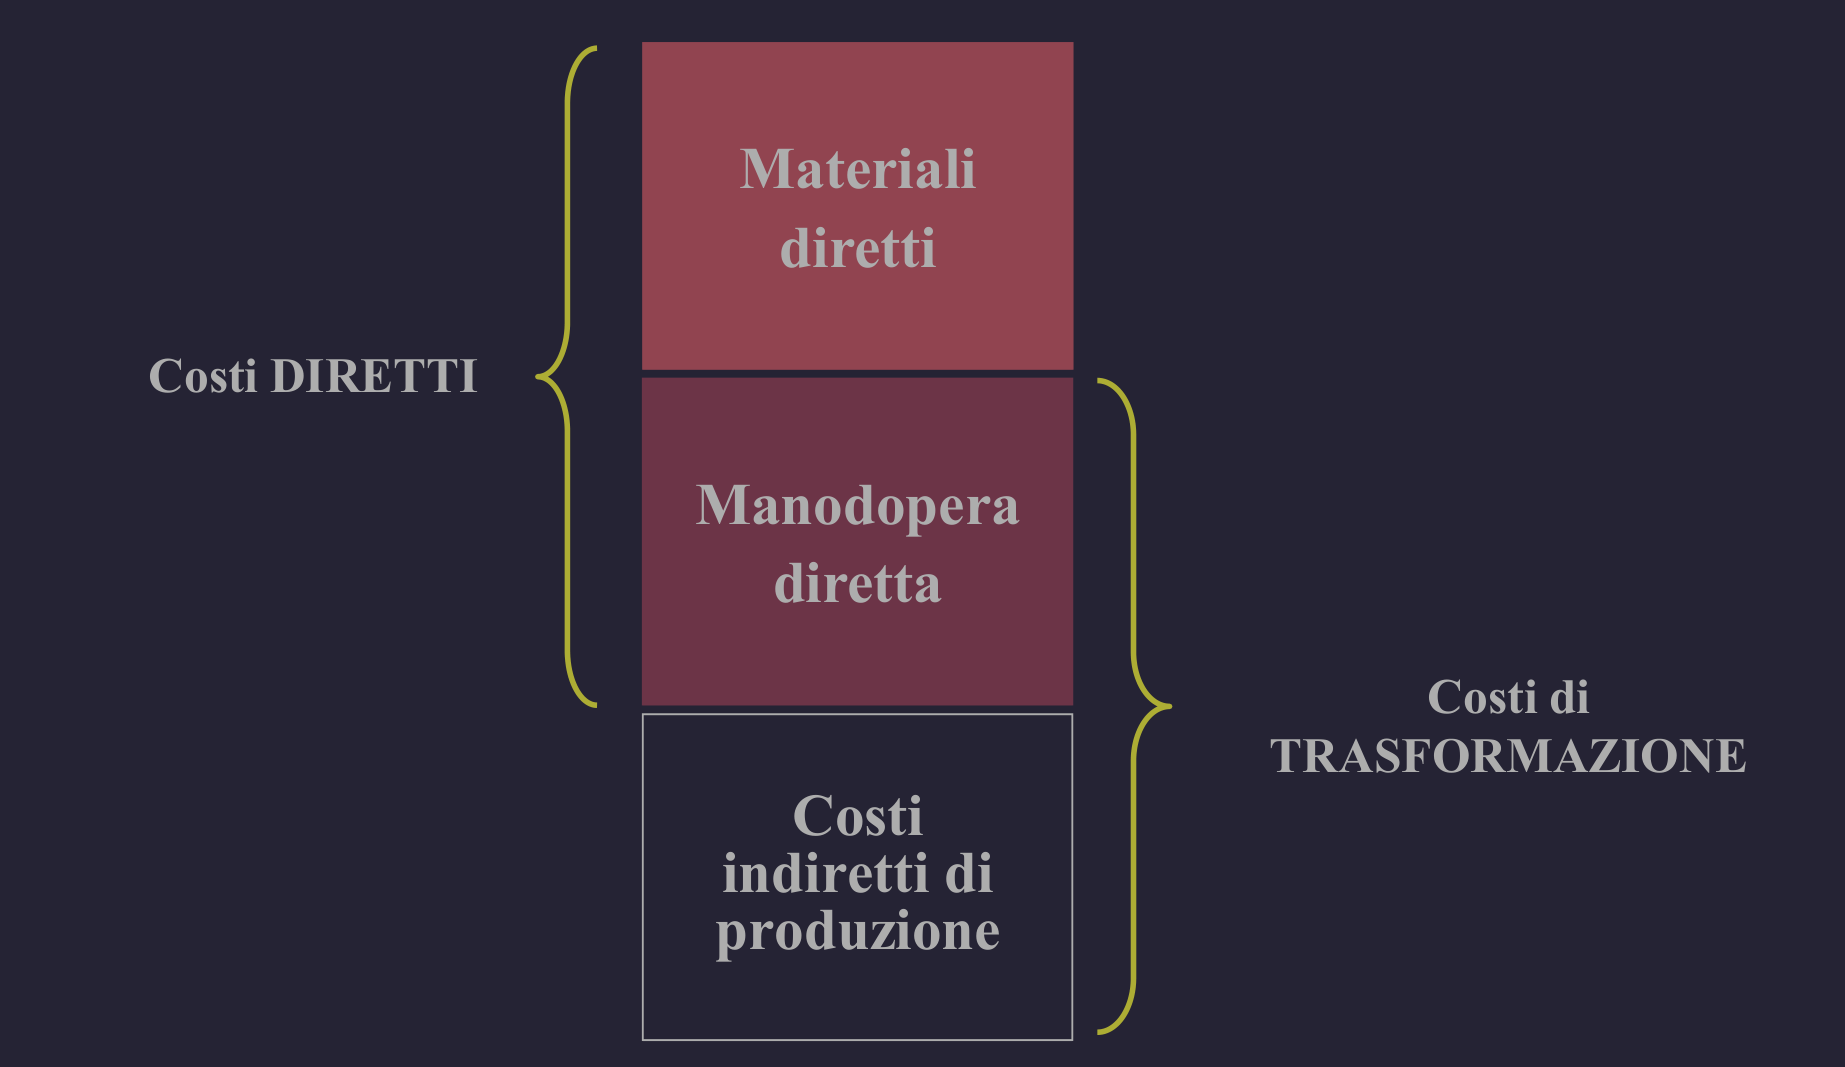
\includegraphics[scale=0.22]{Image/ElemCosto_1.png}
\end{center}
\textbf{N.B.} I costi di trasformazione sono la somma dei costi di tutte le risorse necessarie a trasformare i materiali diretti in prodotto finito.
\vspace*{0.2cm}\\
Definiamo ora i \textbf{costi di periodo:} sono tutti i costi che non rientrano in costi di prodotto (cioè i materiali diretti e i costi di trasformazione), ad esempio i costi di marketing, commerciali, generali e amministrativi.
\begin{center}
    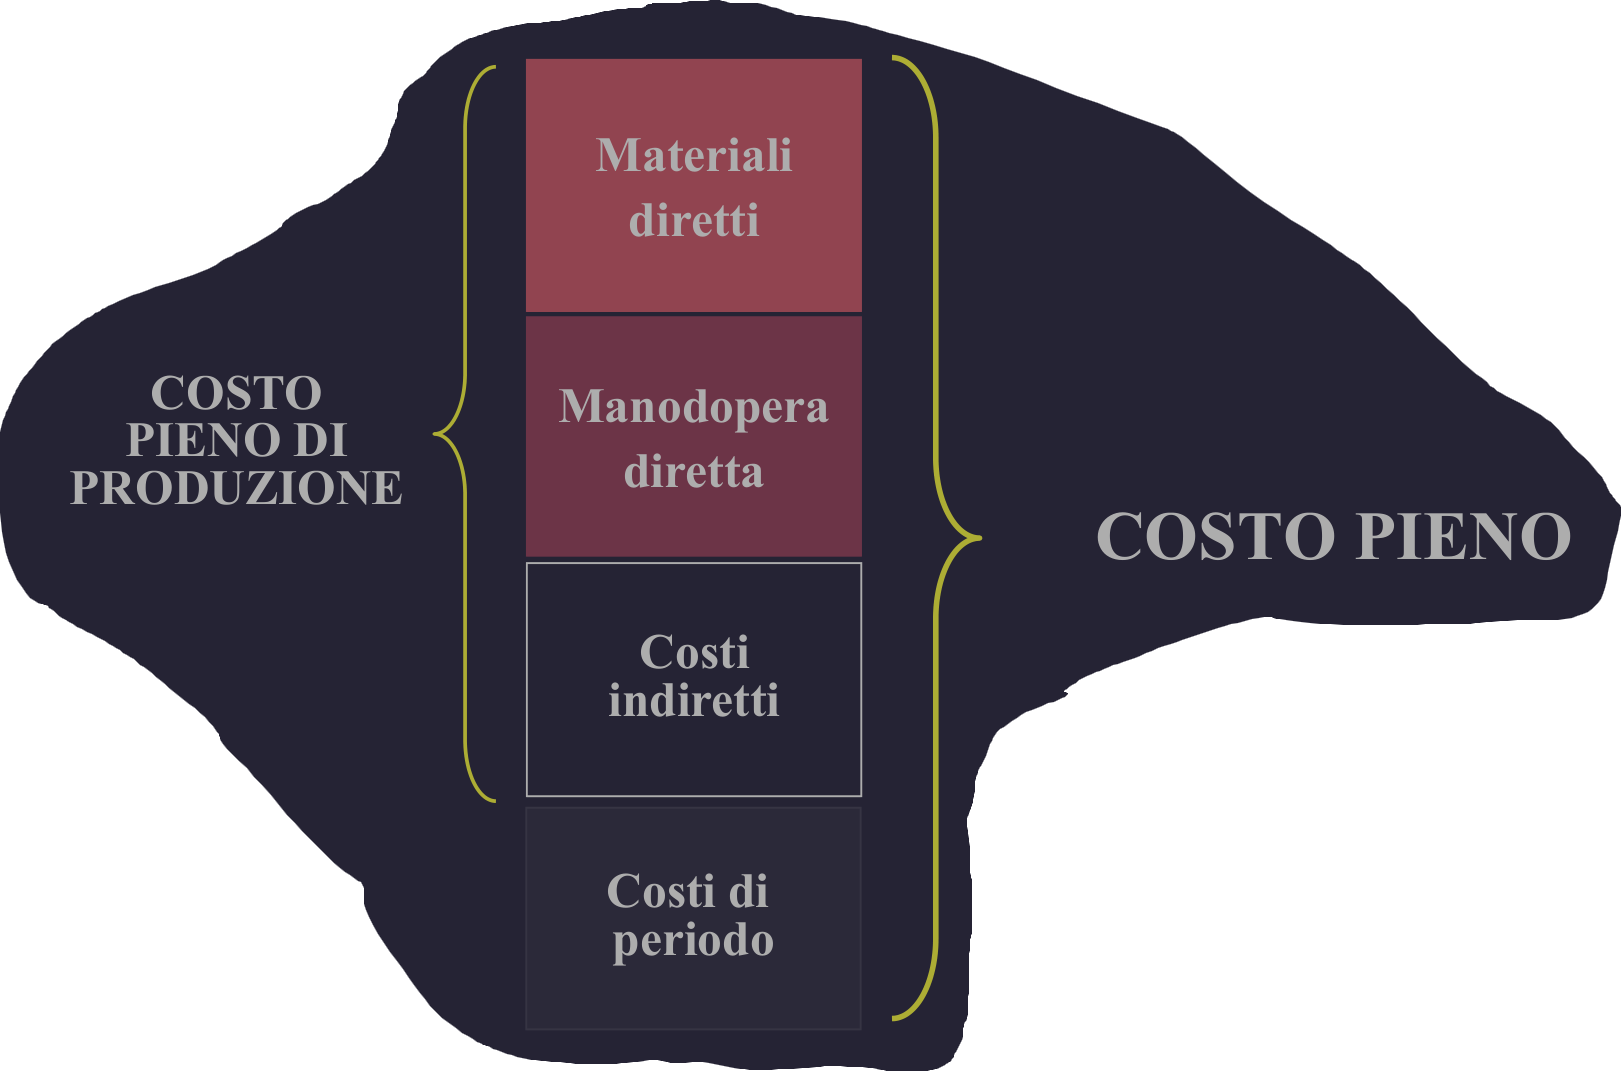
\includegraphics[scale=0.22]{Image/ElemCosto_2.png}
\end{center}



\subsection{Sistema di determinazione dei costi di prodotto (contabilità industriale)}
\begin{center}
    \textit{Il sistema per la rilevazione dei costi è l'insieme delle regole utilizzate per ripartire i costi aziendali tra gli specifici oggetti di costo }
\end{center}
I motivi per cui bisogna capire come determinare i costi di prodotto sono due:
\begin{enumerate}
    \item capire come si determina il valore complessivo delle rimanenze e quello del costo del venduto
    \item sviluppare la base concettuale necessaria a comprendere come i manager utilizzano le informazioni di costo nel processo decisionale
\end{enumerate}
Ci sono due metodi per determinare il costo pieno:
\begin{enumerate}
    \item \textbf{metodo diretto o semplificato:} il procedimento prevede, oltre all'attribuzione dei costi diretti al prodotto, l'allocazione dei costi indiretti, classificati per natura, ai prodotti/servizi
    attraverso l'utilizzo di un'unica base di riparto o su base multipla;
    \item \textbf{metodo per centri di costo:} gli elementi di costo sono in una prima fase accumulati per centri di costo, e in una seconda fase assegnati ai prodotti.
\end{enumerate}


\subsubsection{Metodo diretto o semplificato}
I costi indiretti sono allocati tramite basi di riparto con le quali si determina il coefficiente di allocazione, il quale è la quota di costo indiretto allocabile per ogni unità di base di riparto. 
\[
    \T{Coefficiete di allocazione} = \frac{\T{Costo indiretto da allocare}}{\T{Base di riparto}}
\]
Ad esempio, si ipotizzi un'azienda con due prodotti (A e B); i costi diretti totali di A e B sono rispettivamente pari a €300.000 e €400.000, le quantità di vendita sono pari a 3.000 e 2.000, i costi indiretti ammontano a €100.000. Si determini il costo pieno sapendo che i costi indiretti sono allocati sulla base dei volumi di vendita.
\[
    \T{Coefficiente di allocazione} = \frac{100.000\T{\euro}}{3.000+2.000} = 20 \T{\euro}  
\]
Quota di costi indiretti di A: $20\T{\euro} \times 3.000  = 60.000 \T{\euro}$\\
Quota di costi indiretti di B: $20\T{\euro} \times 2.000  = 40.000 \T{\euro}$\\
\begin{center}
    \begin{tabular}{|c|c|c|}
        \hline 
        & A & B \\ \hline
        Quota equa costi indiretti & 60.000\euro & 40.000\euro \\ \hline
        Costo pieno di produzione & 360.000\euro & 440.000\euro \\ \hline
        Costo pieno unitario & 120\euro & 220\euro\\ \hline 
    \end{tabular}
\end{center}


\subsubsection{Vantaggi e svantaggi del metodo diretto}
\begin{center}
    \begin{tabular}{|m{5cm}|m{5cm}|}
        \hline 
        \textbf{Vantaggi} & \textbf{Svantaggi} \\ \hline
        Elevata semplicità di progettazione e di utilizzo & Elevata approssimazione dei criteri di allocazione dei costi indiretti \\ 
        Velocità di analisi e di elaborazione dei dati & Ridotta capacità di comprendere l'effettiva causa dei costi indiretti \\ 
        Limitati costi di gestione & Assente capacità di cogliere l'influenza dei fattori di complessità produttiva generati dei prodotti\\ \hline 
    \end{tabular}
\end{center}


\subsubsection{Le basi di allocazione più diffuse}
Le basi di allocazione “convenzionali” allocano i costi comuni in proporzione al consumo di risorse dirette, dunque in proporzione ai volumi.
\begin{center}
    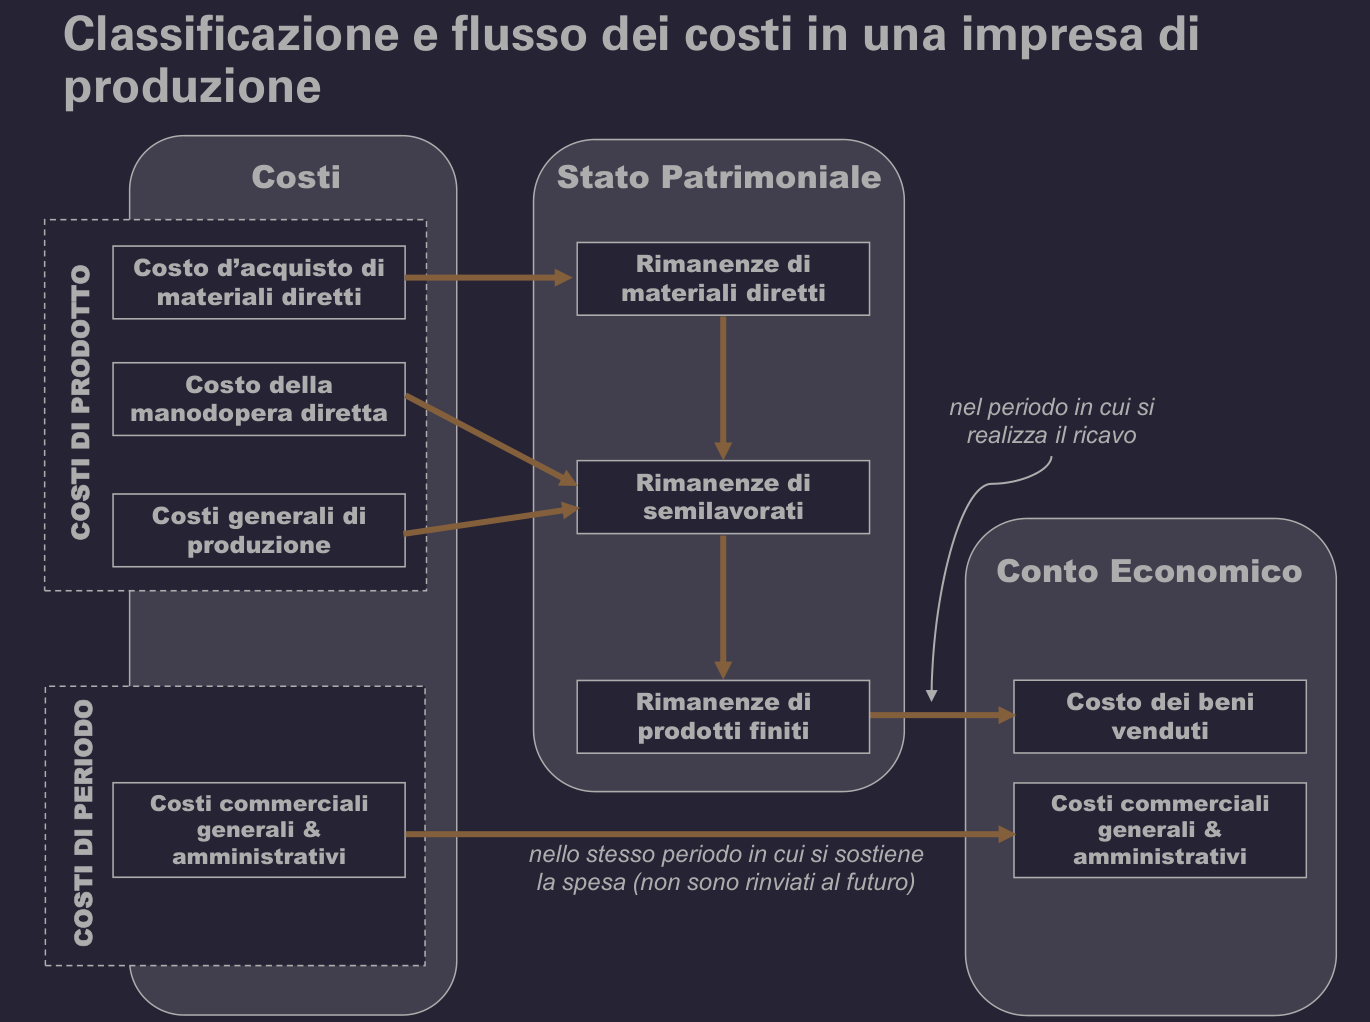
\includegraphics[scale=0.25]{Image/BasiAlloc_1.png}
\end{center}


\subsection{L'uso del costo pieno}
Gli utilizzi del \textit{costo pieno}, che ne sottolineano la rilevanza, sono molteplici:
\begin{itemize}
    \item valorizzare le rimanenze nello stato patrimoniale e il costo del venduto nel conto economico;
    \item svolgere un'\textit{analisi di redditività}: permette di valutare la redditività di un prodotto, di una linea di prodotto, o di uno stabilimento;
    \item rispondere banalmente alla domanda "quant`è costato?"
    \item definire il prezzo "normale" che ci permette di recuperare i costi diretti, una quota di costi indiretti  e generare un reddito soddisfacente
\end{itemize}


\subsubsection{La gestione strategica dei costi}
La \textit{gestione strategica dei costi} definisce come si posizione economicamente l'impresa all'interno del \textbf{sistema del valore} (chiamato anche catena del valore o filiera).\\
Il sistema di valore è l'insieme di tutte le attività necessarie alla realizzazione del prodotto, dall'estrazione delle materie prime ai servizi di assistenza post vendita.
\begin{center}
    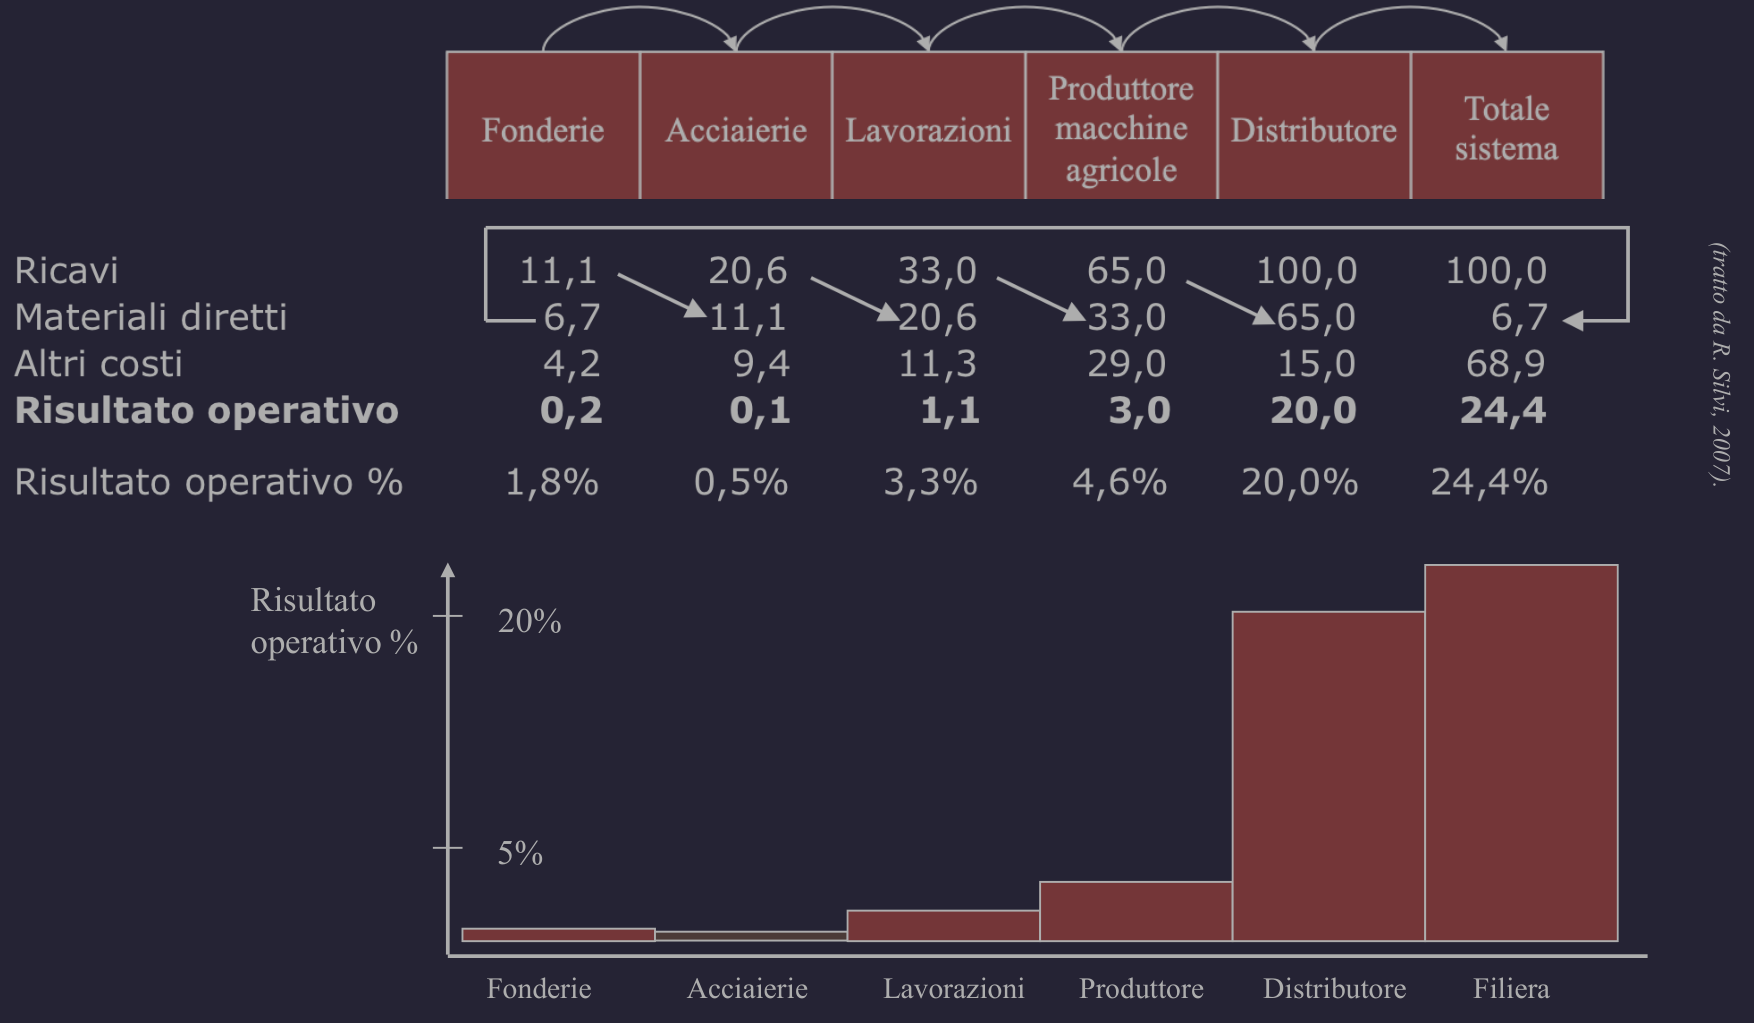
\includegraphics[scale=0.3]{Image/GestStrategica_1.png}
\end{center}

\subsection{Esercizio Cheap Stuff}
L'azienda manifatturiera Cheap Stuff Spa, nella sua sede di Pechino, produce tre tipi differenti di artefatti industriali in materiale ceramico: nano con cappello, nano con fungo e nano guerriero. Nel prospetto seguente sono riportate alcune informazioni relative alla realizzazione di questi prodotti nel corso dell'anno 2005.
\begin{center}
    \begin{tabular}{|l|c|c|c|}
        \hline
        & Nano con cappello & Nano con fungo & Nano guerriero\\ \hline
        Prezzo unitario (€/pezzo)&32&20&14 \\ \hline
        Costo manodopera (€/ora)&10&10&10 \\ \hline
        Costo materie prime (€/kg)&14&10&5 \\ \hline
        Costo verniciatura (€/pezzo)&3&3&3 \\ \hline
        Materie prime (kg/pezzo)&1&0,8&0,8 \\ \hline
        Numero di unità prodotte e vendute (in unità)&112.000&228.700&120.000 \\ \hline
        Tempo unitario di produzione (min/pezzo)&9&4&1,5 \\ \hline
    \end{tabular}
\end{center}
\begin{center}
    \begin{tabular}{|l|c|}
        \hline
        Ammortamento dell'impianto (€)&300.000 \\ \hline
        Spese generali e amministrative (€)&1.000.000 \\ \hline
        Spese commerciali (€)&500.000 \\ \hline
    \end{tabular}
\end{center}
Si chiede di:
\begin{enumerate}
    \item Trovare il margine di contribuzione dei tre prodotti;
    \item Calcolare costo pieno unitario dei tre prodotti, considerando che l'allocazione dell'ammortamento avviene sulla base del tempo di produzione, mentre per le spese generali, amministrative e commerciali si utilizzano i ricavi come base di allocazione;
    \item Il profitto totale generato dalla produzione e commercializzazione dei tre prodotti.
\end{enumerate}

\subsubsection*{Domanda 1: Trovare il margine di contribuzione dei prodotti}
Margine di contribuzione = prezzo unitario - costo variabile unitario
I costi variabile riportati sono:
\begin{itemize}
    \item Costo manodopera (€/ora);
    \item Costo materie prime (€/kg);
    \item Costo verniciatura (€/pezzo).
\end{itemize}
Dobbiamo trasformare i costi di manodopera e materie prime da €/ora e €/kg in €/pezzo, dato che conosciamo il prezzo unitario, il quale è calcolato in €/pezzo.

\subsubsection*{Costo manodopera per pezzo}
Nano con cappello:\\
$10/60 \  \T{\euro} / min \times 9\  min/pezzo = 1,50 \T{\euro}/pezzo $
\vspace*{0.2cm}\\
Nano con fungo:\\
$10/60 \ \T{\euro} / min \times 4\ min/pezzo = 0,67 \T{\euro}/pezzo $
\vspace*{0.2cm}\\
Nano guerriero:\\
$10/60 \ \T{\euro} / min \times 1,5\ min/pezzo = 0,25 \T{\euro}/pezzo $

\subsubsection*{Costo materie prime per pezzo}
Nano con cappello (1 kg/pezzo):\\
14 €/pezzo
\vspace*{0.1cm}\\
Nano con fungo (0,8kg/pezzo):\\
$ 0,8\ kg/pezzo \times 10\ \T{\euro}/kg = 8 \T{\euro}/pezzo $
\vspace*{0.1cm}\\
Nano guerriero (0,8kg/pezzo):\\
$ 0,8\ kg/pezzo \times 5\ \T{\euro}/kg = 4 \T{\euro}/pezzo $

\subsubsection*{Costo variabile}
Il costo variabile sarà quindi dato dall'equazione : Costo Variabile = Costo Manodopera + Costo Materie Prime + Costo Verniciatura.
\vspace*{0.1cm}\\
Nano con cappello:\\
Costo variabile = 1,5 + 14 + 3 = \textbf{18,50 €}
\vspace*{0.1cm}\\
Nano con fungo:\\
Costo variabile = 0,67 + 8 + 3 = \textbf{11,67 €}
\vspace*{0.1cm}\\
Nano guerriero:\\
Costo variabile = 0,25 + 4 + 3 = \textbf{7,25 €}
\vspace*{0.2cm}\\

\subsubsection{Domanda 1: Margine di contribuzione}
Margine di contribuzione=Prezzo unitario - Costo variabile
\vspace*{0.2cm}\\
Nano con cappello:\\
32-18,50 = 13,50 \euro 
\vspace*{0.1cm}\\
Nano con fungo:\\
20-11,67 = 8,33 \euro 
\vspace*{0.1cm}\\
Nano guerriero:\\
14-7,25 = 6,75 \euro 

\subsubsection{Domanda 2: Calcolo costo pieno unitario}
Il costo pieno del prodotto è calcolato utilizzando i costi unitari: costo manodopera diretta + costo materiali diretti + costi indiretti di produzione + costi di periodo.\\
I costi indiretti (ammortamento dell'impianto) e i costi di periodo (spese generali e amministrative) devono essere allocati tramite basi di riparto. Il primo step per calcolare il costo pieno è definire il coefficiente di allocazione di questi costi.
\[
    \T{Coefficiente di allocazione} = \T{Costo indiretto da allocare}/\T{Base di riparto}
\]
La base del costo dell'ammortamento è il tempo di produzione, mentre la base dei costi spese generali e amministrative e spese commerciali si utilizzano i ricavi.

\subsubsection*{Coefficiente di allocazione ammortamento}
Ammortamento: 300,000 \euro 
\vspace*{0.2cm}\\
Nano con cappello:\\
Tempo totale di produzione = $\underbrace{112.000}_{\substack{\text{unità} \\ \text{prodotte}}} \times \underbrace{9 \T{ min}}_{\substack{\text{tempo di} \\ \text{produzione} \\ \text{unitario}}} = 1.008.000 \T{ min} $
\vspace*{0.1cm}\\
Nano con fungo:\\
Tempo totale di produzione = $\underbrace{228.700}_{\substack{\text{unità} \\ \text{prodotte}}} \times \underbrace{4 \T{ min}}_{\substack{\text{tempo di} \\ \text{produzione} \\ \text{unitario}}} = 914.800 \T{ min} $
\vspace*{0.1cm}\\
Nano guerriero:\\
Tempo totale di produzione = $\underbrace{120.000}_{\substack{\text{unità} \\ \text{prodotte}}} \times \underbrace{1,5 \T{ min}}_{\substack{\text{tempo di} \\ \text{produzione} \\ \text{unitario}}} = 180.000 \T{ min} $
\vspace*{0.1cm}\\
Tempo totali di produzione impianto = $1.008.000 + 914.800 + 180.000 = 2.102.800$ min
Coefficiente di allocazione (ammortamento) = $300.000/2.102.800 = 0,14267 $

\subsubsection*{Coefficiente di allocazione spese generali e amministrative}
Spese generali e amministrative = 1.000.000 €
\vspace*{0.2cm}\\
Nano con cappello:\\
Fatturato = $\underbrace{112.000}_{\substack{\text{unità} \\ \text{prodotte}}} \times \underbrace{32 \T{\euro}}_{\substack{\text{prezzo} \\ \text{unitario}}} = 3.584.00  \T{\euro} $
\vspace*{0.1cm}\\
Nano con fungo:\\
Fatturato = $\underbrace{228.700}_{\substack{\text{unità} \\ \text{prodotte}}} \times \underbrace{20 \T{\euro}}_{\substack{\text{prezzo} \\ \text{unitario}}} = 4.574.00  \T{\euro} $
\vspace*{0.1cm}\\
Nano guerriero:\\
Fatturato = $\underbrace{112.000}_{\substack{\text{unità} \\ \text{prodotte}}} \times \underbrace{32 \T{\euro}}_{\substack{\text{prezzo} \\ \text{unitario}}} = 1.680.00 \T{\euro} $
\vspace*{0.1cm}\\
Totale fatturato = $3.584.000 + 4.574.000 + 1.680.000 = 9.838.000$\euro\\
Coefficiente di allocazione (spese g.a.) = $1.000.000/9.838.000 = 0,1016$

\subsubsection*{Coefficiente di allocazione spese commerciali}
Spese commerciali = 500.000\euro 
Anche le spese commerciali sono allocate su base dei ricavi, quindi riutilizziamo il fatturato totale calcolato in precedenza.
\vspace*{0.2cm}\\
Coefficiente di allocazione (spese comm.) = $500.000/9.838.000 = 0,0508$

\subsubsection*{Secondo step: calcolo costo indiretto unitario}
\subsubsection*{Ammortamento}
Ora calcoliamo il costo dell'\textbf{\underline{ammortamento}} impianto per pezzo: siccome l'ammortamento è allocato sulla base del tempo di produzione dobbiamo prendere le ore di produzione di ogni prodotto e moltiplicarle per il coefficiente di allocazione, dopodiche dividere per il totale delle unità prodotte.
\vspace*{0.1cm}\\
Nano con cappello:\\
Ammortamento impianto per pezzo = $ \dfrac{\overbrace{1.008.000}^{\substack{\text{ore di} \\ \text{produzione}}} \times \overbrace{0,14267}^{\substack{\text{coefficiente} \\ \text{allocazione}}}}{\underbrace{112.000}_{\substack{\text{unità} \\ \text{prodotte}}}}=1,28\T{\euro} $
\vspace*{0.1cm}\\
Nano con fungo:\\
Ammortamento impianto per pezzo = $ \dfrac{\overbrace{914.800}^{\substack{\text{ore di} \\ \text{produzione}}} \times \overbrace{0,14267}^{\substack{\text{coefficiente} \\ \text{allocazione}}}}{\underbrace{228.700}_{\substack{\text{unità} \\ \text{prodotte}}}}=0,57\T{\euro} $
\vspace*{0.1cm}\\
Nano guerriero:\\
Ammortamento impianto per pezzo = $ \dfrac{\overbrace{180.000}^{\substack{\text{ore di} \\ \text{produzione}}} \times \overbrace{0,14267}^{\substack{\text{coefficiente} \\ \text{allocazione}}}}{\underbrace{120.000}_{\substack{\text{unità} \\ \text{prodotte}}}}=0,21\T{\euro} $


\subsubsection*{Spese generali e amministrative}
Per le \textbf{\underline{spese generali e amministrative}} si moltiplica il coefficiente di allocazione per il ricavo di ogni prodotto e dopo dividere per il numero di unità prodotte e vendute.
\vspace*{0.2cm}\\
Nano con cappello:\\
Spese generali e amministrative per pezzo = $ \dfrac{\overbrace{3.584.000}^{\text{fatturato}} \times \overbrace{0,1016}^{\substack{\text{coefficiente} \\ \text{allocazione}}}}{\underbrace{112.000}_{\substack{\text{unità} \\ \text{prodotte}}}}=1,28\T{\euro}$
\vspace*{0.1cm}\\
Nano con fungo:\\
Spese generali e amministrative per pezzo = $ \dfrac{\overbrace{4.574.000}^{\text{fatturato}} \times \overbrace{0,1016}^{\substack{\text{coefficiente} \\ \text{allocazione}}}}{\underbrace{228.700}_{\substack{\text{unità} \\ \text{prodotte}}}}=2,03\T{\euro}$
\vspace*{0.1cm}\\
Nano guerriero:\\
Spese generali e amministrative per pezzo = $ \dfrac{\overbrace{1.680.000}^{\text{fatturato}} \times \overbrace{0,1016}^{\substack{\text{coefficiente} \\ \text{allocazione}}}}{\underbrace{120.000}_{\substack{\text{unità} \\ \text{prodotte}}}}=1,42\T{\euro}$


\subsubsection*{Spese commerciali}
Nano con cappello:\\
Spese commerciali per pezzo = $ \dfrac{\overbrace{3.584.000}^{\text{fatturato}} \times \overbrace{0,0508}^{\substack{\text{coefficiente} \\ \text{allocazione}}}}{\underbrace{112.000}_{\substack{\text{unità} \\ \text{prodotte}}}}=1,63\T{\euro}$
\vspace*{0.1cm}\\
Nano con fungo:\\
Spese commerciali per pezzo = $ \dfrac{\overbrace{4.574.000}^{\text{fatturato}} \times \overbrace{0,0508}^{\substack{\text{coefficiente} \\ \text{allocazione}}}}{\underbrace{228.700}_{\substack{\text{unità} \\ \text{prodotte}}}}=1,02\T{\euro}$
\vspace*{0.1cm}\\
Nano guerriero:\\
Spese commerciali per pezzo = $ \dfrac{\overbrace{1.680.000}^{\text{fatturato}} \times \overbrace{0,0508}^{\substack{\text{coefficiente} \\ \text{allocazione}}}}{\underbrace{120.000}_{\substack{\text{unità} \\ \text{prodotte}}}}=0,71\T{\euro}$

\subsubsection*{Terzo step: sommare i costi}
Ora si sommano tutti i costi per trovare il costo pieno per prodotto: Costo manodopera diretta + Costo Materiali diretti + Costi Indiretti di Produzione + Costi di Periodo.
\vspace*{0.2cm}\\
Nano con cappello:\\
Costo pieno = 1,50 + 14 + 3 + 1,28 + 3,25 + 1,63 = 24,66\euro 
\vspace*{0.2cm}\\
Nano con fungo:\\
Costo pieno = 0,67 + 8 + 3 + 0,57 + 2,03 + 1,02 = 15,29\euro 
\vspace*{0.2cm}\\
Nano Guerriero:\\
Costo Pieno = 0,25 + 4 + 3 + 0,21 + 1,42 + 0,71 = 9,59\euro 


\subsubsection{Domanda 3: Profitto totale}
Sappiamo che il profitto si calcola: Profitto = Ricavi - Costo. Calcolo il costo moltiplicando il costo pieno per le unità prodotte e vendute.
\vspace*{0.2cm}\\
Nano con cappello:\\
Profitto = $ 3.584.000 - (24,66 \times 112.000) = 822.080$\euro 
\vspace*{0.1cm}\\
Nano con Fungo:\\
Profitto = $4.574.000 - (15,29 * 228.700)= 1.077.177$\euro 
\vspace*{0.2cm}\\
Nano Guerriero:\\
Profitto = $1.680.000 - (9,59 * 120.000) = 529.200$\euro 
\vspace*{0.2cm}\\
Profitto totale = $ 822.080 + 1.077.177 + 529.200 = 2.428.457$\euro   






\section{Sistemi di determinazione dei costi}
\subsection{Introduzione}
Ricordiamo di seguito gli elementi di costo del prodotto
\begin{center}
    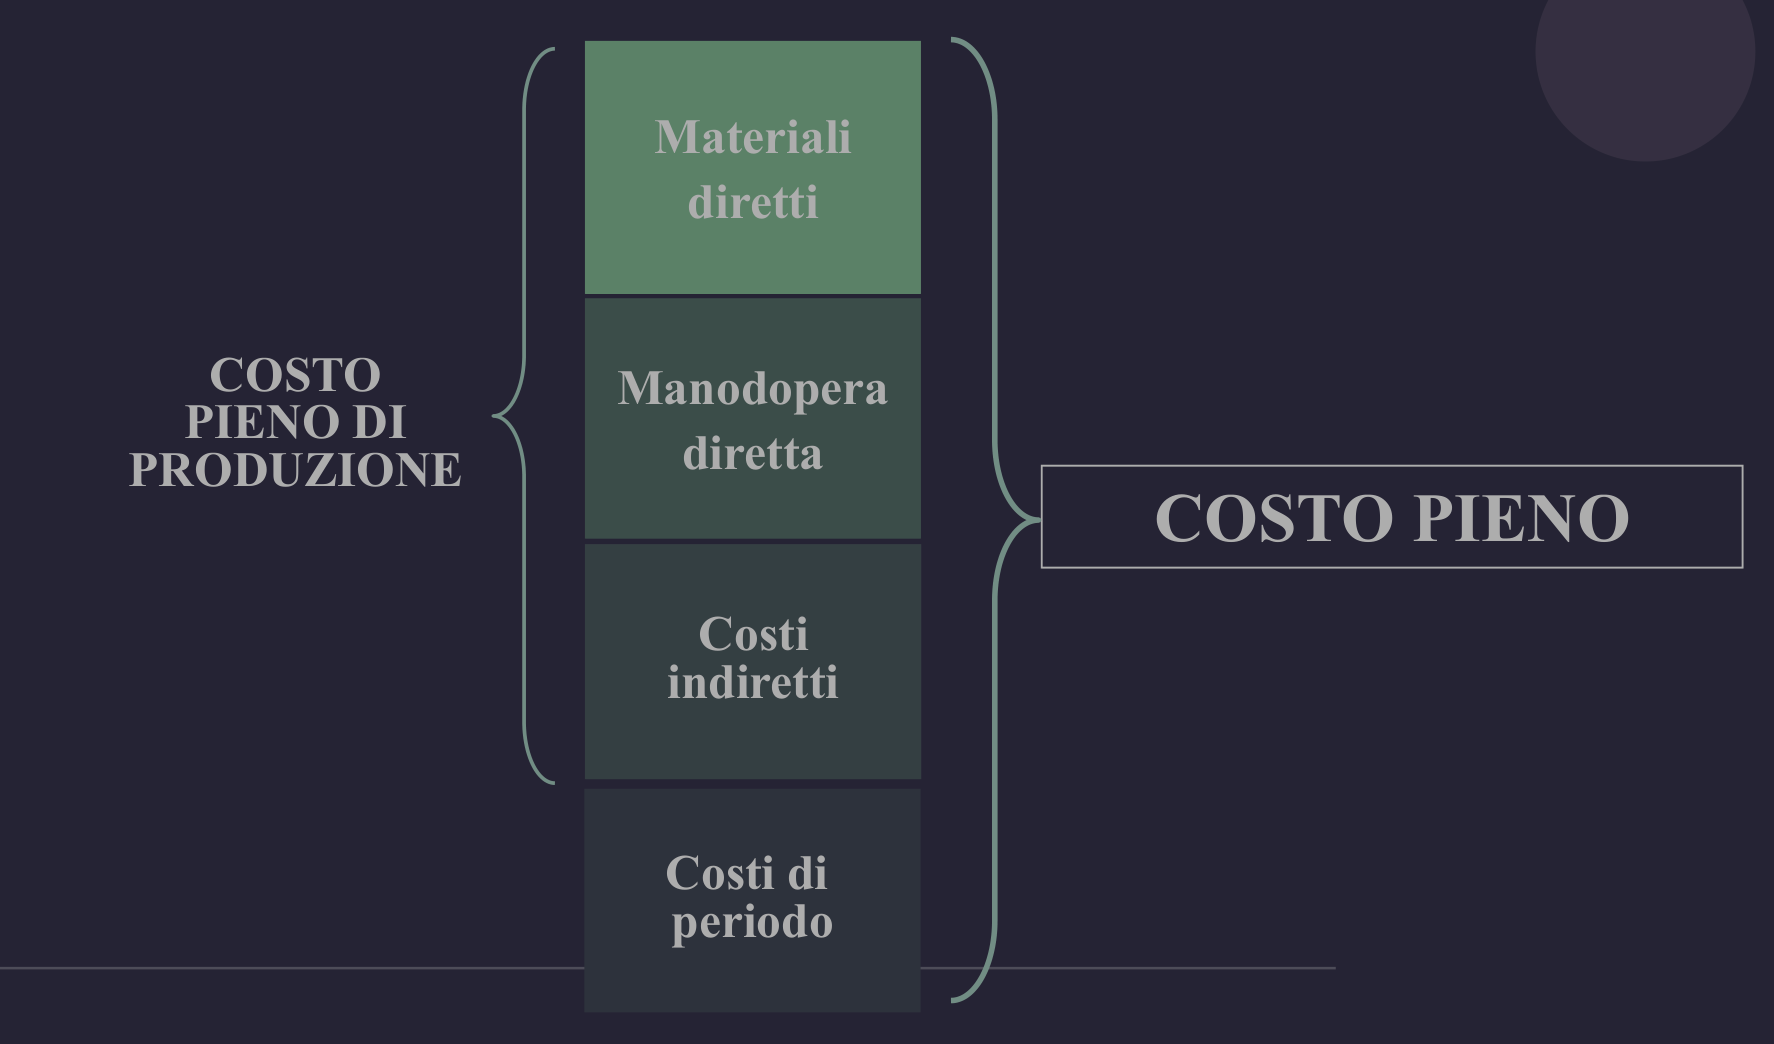
\includegraphics[scale=0.3]{Image/ElemCosto_3.png}
    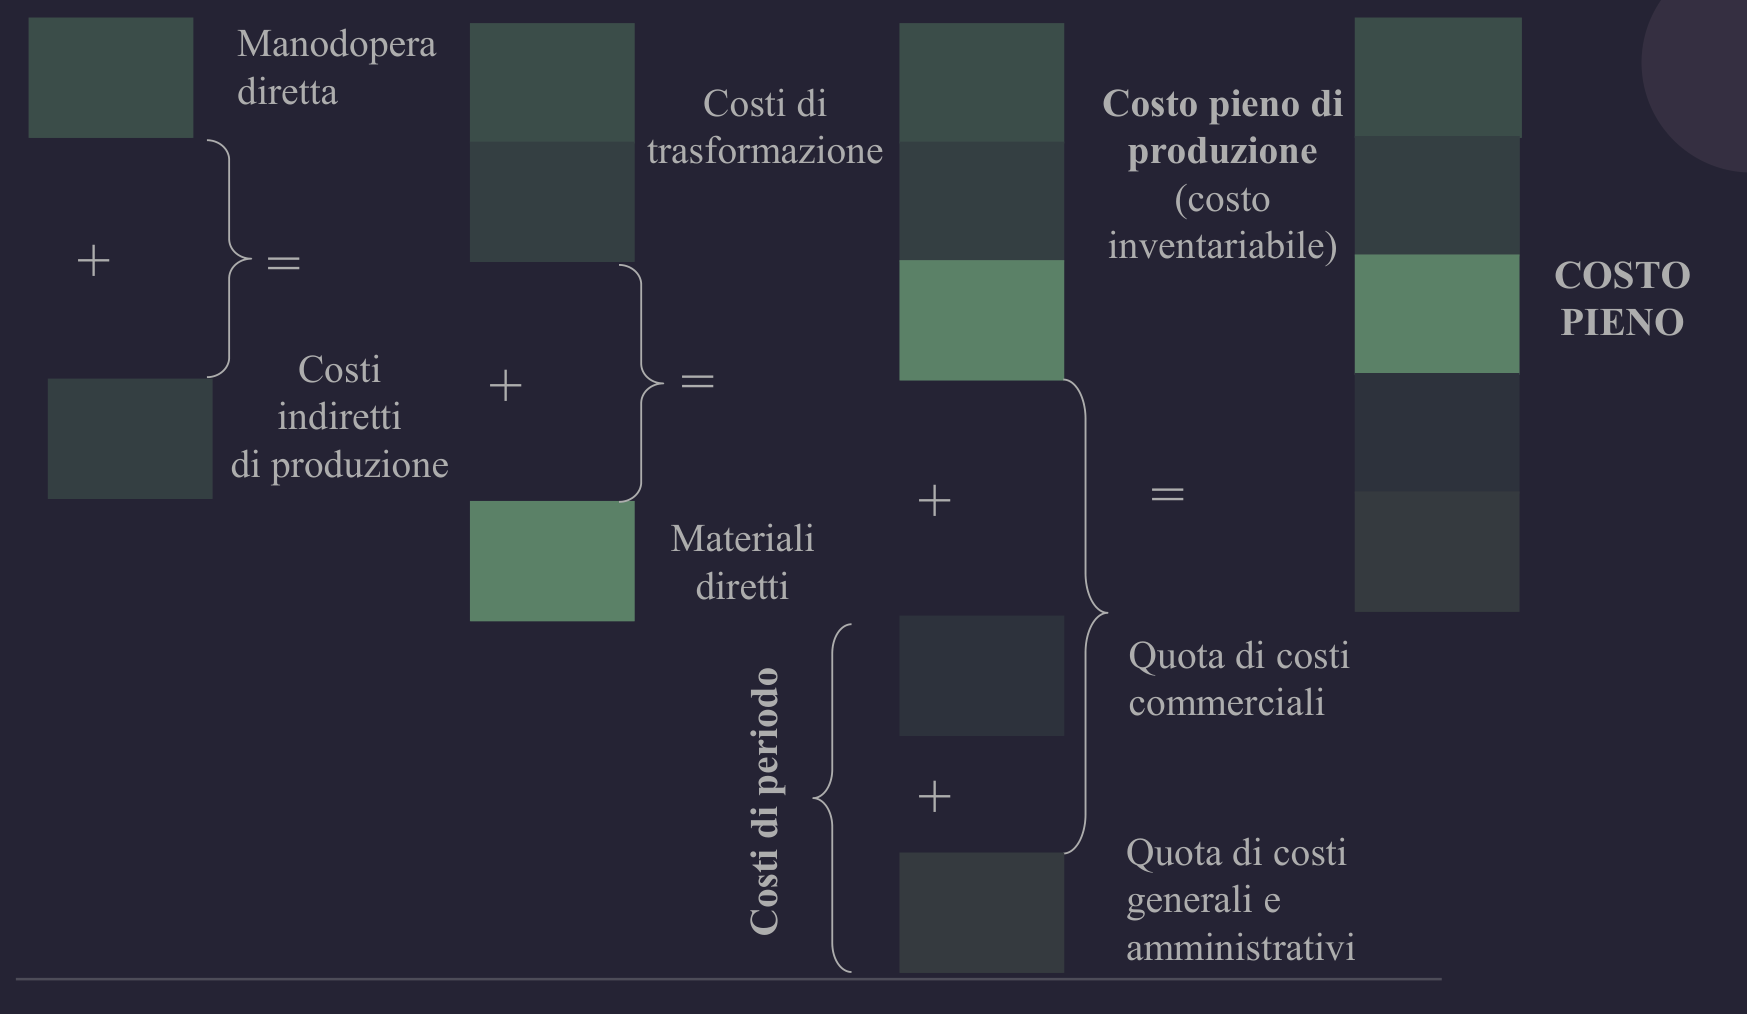
\includegraphics[scale=0.3]{Image/ElemCosto_4.png}
\end{center}
Ricordiamo anche che ci sono due metodi tradizionali per determinare il costo pieno, ma noi ci focalizziamo sul metodo diretto o semplificato, il quale prevede:
\begin{enumerate}
    \item l'attribuzione dei costi diretti al prodotto
    \item l'allocazione dei costi indiretti, classificati per natura, ai prodotti/servizi attraverso l'utilizzo di un'unica base di riparto o su base multipla, con le quali si determina il coefficiente di allocazione
\end{enumerate}
Il coefficiente di allocazione si calcola
\[
    \frac{\T{Costo indiretto da allocare}}{\T{Base di riparto}}
\]


\subsection{Il sistema di determinazione dei costi}
\underline{Il sistema di determinazione dei costi} ci permette di ottenere il costo pieno di produzione dei prodotti; calcola i \textbf{valori medi unitari} di alcune voci di costo. Per quanto riguarda i costi variabili, essi possono anche variare tra i prodotti (per esempio il tempo di manodopera non è esattamente uguale per ogni prodotto, si deve determinare il tempo medio per arrivare al costo di ogni prodotto).
\begin{center}
    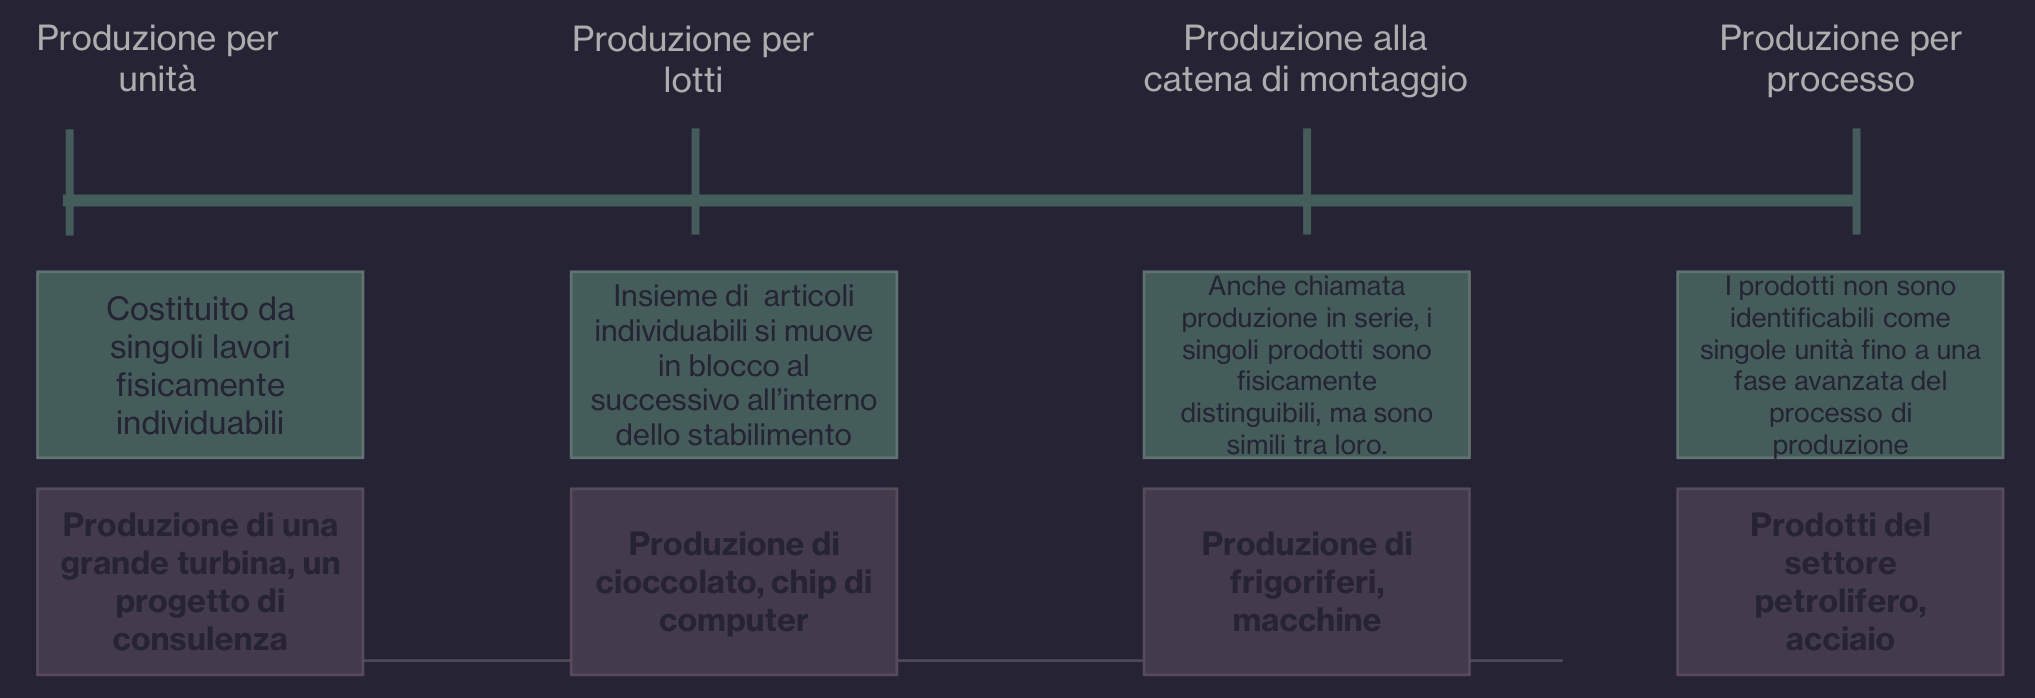
\includegraphics[scale=0.3]{Image/SistCosti_1.png}
\end{center}
Vi sono due sistemi per determinare i costi
\begin{center}
\begin{tabular}{|m{6cm}|m{6cm}|}
    \hline 
    \multicolumn{1}{>{\centering\arraybackslash}m{60mm}|}{\textbf{Sistemi per commessa}}
    & \multicolumn{1}{>{\centering\arraybackslash}m{60mm}|}{\textbf{Sistemi per commesso}}\\ \hline 
    Accumula i costi di ciascun prodotto (o ciascuna commessa) a mano a mano che esso viene realizzato, indipendentemente dal periodo contabile di svolgimento
\end{tabular}
\end{center}

































\end{document}